% filepath: c:\Users\wojte\Desktop\mgr.tex
\documentclass{pracalicmgr}
\usepackage[utf8]{inputenc}
\usepackage{booktabs}
\usepackage{amsmath}
\usepackage{hyperref}
\usepackage{graphicx}
\usepackage{parskip}
\usepackage{setspace}
\usepackage{subcaption}  % Add this line
\usepackage{float}
\usepackage{amsmath}
\usepackage{enumitem}
\usepackage{amsmath}
\usepackage{amssymb}
\usepackage{caption}
\usepackage[utf8]{inputenc}
\usepackage[T1]{fontenc}
\usepackage{amsmath}
\usepackage{amsfonts}
\usepackage{amssymb}
\usepackage{graphicx}
\usepackage{fancyhdr}
\usepackage[utf8]{inputenc}
\usepackage{graphicx}
\usepackage{textcomp}
\usepackage{titlesec}
\usepackage[T1]{fontenc}
\usepackage{float}
\usepackage[english]{babel}
\usepackage{gensymb}
\usepackage{enumitem}
\usepackage{chngcntr}
\usepackage{epstopdf}
\usepackage{color}
\usepackage{indentfirst}
\usepackage{mathtools}
\usepackage{lmodern}
\usepackage{amsfonts}
\usepackage{hyperref}
\usepackage{xurl}
\usepackage{braket}
\usepackage{amsmath}
\usepackage{longtable}


\pagestyle{fancy}
\fancyhf{} % Clear all headers and footers
\fancyfoot[LO,RE]{\thepage} % Left on even pages, right on odd pages
\renewcommand{\headrulewidth}{0pt} % Remove header line

% Redefine plain page style (used on chapter pages) to match fancy style
\fancypagestyle{plain}{%
  \fancyhf{} % Clear all headers and footers
  \fancyfoot[LO,RE]{\thepage} % Left on even pages, right on odd pages
  \renewcommand{\headrulewidth}{0pt} % Remove header line
}
% \usepackage[
%   textheight=24.5cm,
%   textwidth=16cm,
%   top=-0.5cm,
%   headheight=0cm,
%   left=0.5cm,
%   right=-0.2cm,
%   oddsidemargin=0.5cm,
%   evensidemargin=-0.5cm
% ]{geometry}


\usepackage{wrapfig}

%\linespread{2}
\raggedbottom
%\counterwithin{figure}{section}

\author{Wojciech Noskowiak}

\nralbumu{417909}

\title{Event classification in liquid argon time projection chambers using neural networks}

\tytulang{Klasyfikacja zdarzeń w komorach projekcyjnych z ciekłym argonem przy użyciu sieci neuronowych}

\kierunek{Physics}

%\specjalnosc{Metody jądrowe w fizyce ciała stałego}

\opiekun{\\dr hab. Katarzyna Grzelak\\ Institute of Experimental Physics\\ Faculty of Physics, University of Warsaw\\\vspace{0.3cm plus 1.5fill}\\dr hab. Artur Kalinowski\\ Institute of Experimental Physics\\ Faculty of Physics, University of Warsaw \\}

%\dziedzina{13.200}
\dziedzina{13.2 Fizyka}

\date{July 2025}

\keywords{deep learning, convolutional neural networks, transformers, neutrino classification, MicroBooNE, AlexNet, LeNet, image classification, LArTPC}

\overfullrule=1pt
\begin{document}
\setlength{\textheight}{24.5cm}
\setlength{\textwidth}{16cm}
\setlength{\topmargin}{-0.5cm}
\setlength{\headheight}{0cm}
\setlength{\oddsidemargin}{0.5cm}
\setlength{\evensidemargin}{-0.5cm}

\maketitle
\let\cleardoublepage\clearpage

\begin{abstract}
The objective of this thesis was to evaluate the effectiveness of deep learning methods in classifying neutrino interactions in Liquid Argon Time Projection Chambers (LArTPCs), using data from the MicroBooNE OpenSamples dataset. The classification task focused on distinguishing charged current electron neutrino interactions from other types of events. Several neural network architectures were tested: a shallow LeNet-like model, a deeper AlexNet-based convolutional network, and a transformer-based model.The LeNet-like model failed to learn any meaningful features and did not yield usable results. AlexNet-like network achieved high classification performance, reaching accuracies up to 85.97\%. The transformer model achieved reasonable results with an accuracy of 66.03\%. These outcomes suggest that the aforementioned classification task is solvable with current machine learning techniques. Further improvement is likely achievable through training on larger datasets, employing more complex architectures, or including additional input data from other wire planes.

\end{abstract}

\tableofcontents

\chapter*{Introduction}

Neutrinos are fundamental particles that come in three known types (also referred to as flavors). They interact only via the weak nuclear force, making them difficult to detect. In the late 1960s, experiments observed a deficit in the number of solar neutrinos, which was later explained by the phenomenon of neutrino oscillations, which have since been the subject of extensive experimental and theoretical investigation\cite{NeutrionoOscillationsHistory}. The mechanism by which neutrinos acquire mass remains unknown, since their masses have not yet been measured.

In addition, several experimental anomalies have been reported that deviate from the predictions of the three-flavor neutrino oscillation model. These include results from the LSND and MiniBooNE experiments, as well as the reactor neutrino anomaly. In all cases, the observed number of neutrinos does not align with the expectations derived from standard oscillation models\cite{neutrinoAnomally}.

One possible explanation for these discrepancies involves extending the current model by introducing additional neutrino flavors. In particular, the hypothesis of sterile neutrinos — neutrinos that do not interact via the weak nuclear force—has been proposed. If such a hypothesis were to be confirmed, it would require an extension of the Standard Model of particle physics. These potential non-interactive neutrinos have even been considered as potential candidates for dark matter\cite{neutrinoDarkMatter}.

Neutrino oscillations—both standard and non-standard—have so far been studied primarily using water or ice based Cherenkov detectors and scintillation detectors. More recently, liquid argon (LAr) detectors have started being more commonly deployed. One of the largest currently operating LAr detectors is the 170-ton MicroBooNE detector at Fermilab, which was built primarily to investigate the excess of electron neutrino events observed in the MiniBooNE experiment. At the same time, MicroBooNE serves as a testbed for the future large-scale (planned 40 kt) LAr detector—DUNE. (A more detailed discussion of DUNE will be presented in Chapter 2.)

These detectors offer superior spatial resolution to their predecessors, and efficient analysis and interpretation of data produced by the aforementioned detectors still poses a set of open problems, efficient 
identification and classification of different types of neutrino interactions being one of them. 

In this work, a selection of machine learning methods (namely convolutional neural networks and transformers) for selecting electron neutrino interactions is developed and explored. Specifically, it investigates and implements selected approaches and evaluates their performance using the publicly available MicroBooNE OpenSamples dataset.

\chapter{Neutrinos}

\section{Iterations}

\begin{figure}[h]
    \centering
    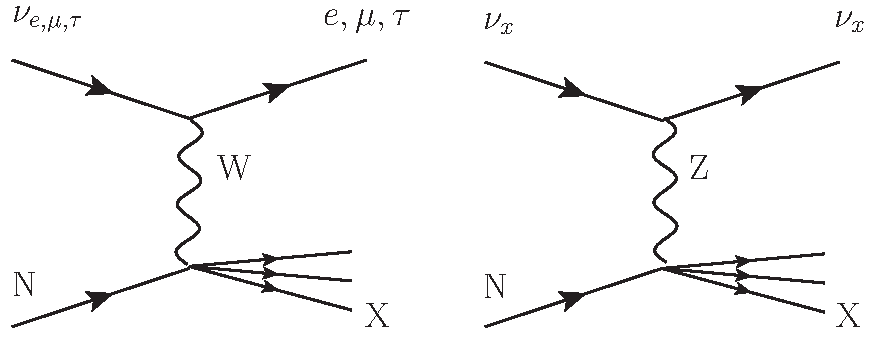
\includegraphics[width=0.55\textwidth]{src/xfig1_3nu.pdf}
    \caption{Feynman diagram illustrating neutrino interactions.\cite{neutrinoFeynmann}}
    \label{fig:Feynman_diagram_neutrino}
\end{figure}

Neutrinos are electrically neutral, spin-$\frac{1}{2}$ elementary particles that belong to the lepton family within the Standard Model of particle physics. They exist in three distinct flavors, corresponding to the three charged leptons: the electron neutrino ($\nu_e$), the muon neutrino ($\nu_\mu$), and the tau neutrino ($\nu_\tau$).\cite{neutrinoFeynmann}

These flavor classifications arise from the weak decay processes mediated by the $W$ boson, in which a charged lepton is produced alongside a corresponding neutrino. For instance, in a $W^-$ decay producing an electron, an electron neutrino is emitted; similarly, decays yielding a muon or tau lepton produce a muon or tau neutrino, respectively.

Due to their lack of electric charge, negligible mass, and absence of color charge, neutrinos interact with matter only via the weak nuclear force. This interaction occurs through two fundamental mechanisms: neutral current interactions, mediated by the electrically neutral $Z^0$ boson, and charged current interactions, mediated by the charged $W^+$ or $W^-$ bosons. Feynman diagrams of these interactions are shown in figure~\ref{fig:Feynman_diagram_neutrino}.

In charged current interactions, the neutrino exchanges a $W$ boson with a target particle, resulting in the production of a charged lepton of the same flavor, which enables neutrino flavor identification. In contrast, neutral current interactions involve the exchange of a $Z^0$ boson and therefore do not produce a charged lepton. The neutriono flavour cannot therefore be deduced from the final state.

The weak interaction is characterized by a very short range, typically on the order of $10^{-17}$ to $10^{-18}$ meters\cite{WeakInteraction}, which makes neutrino interactions with matter extremely rare. As a result, detecting neutrinos requires either very intense neutrino beams and/or very large detectors to observe a statistically significant number of interactions.

\section{Liquid Argon Detectors}

\subsection{Operating principle}

\begin{figure}[H]
    \centering
    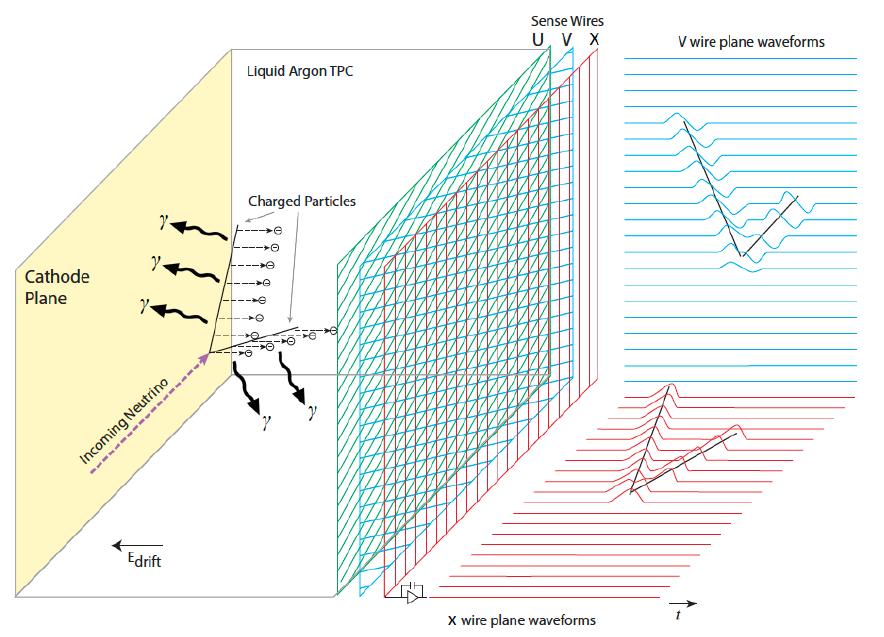
\includegraphics[width=0.7\textwidth]{src/LAr_diagram_DUNE.png}
    \caption{General mechanism of a liquid argon detector (LArTPC).\cite{MicroBooNEDesign}}
    \label{fig:lartcp}
\end{figure}

LArTPC detectors consist of a large chamber filled with liquid argon. Charged particles traversing the chamber leave trails of ionized electrons. An applied electric field causes these electrons to drift toward the anode, where they are detected. Simultaneously, vacuum ultraviolet (VUV) scintillation photons are emitted and collected by photodetectors. The general mechanism of a liquid argon detector is shown in Figure~\ref{fig:lartcp}.

Argon is chosen as the detection medium because it is a noble gas, which is chemically inert and allows for efficient ionization and scintillation. In its liquid state, argon has a high density, enhancing the probability of neutrino interactions. Importantly, argon does not capture ionization electrons, allowing them to drift over long distances without recombination—provided the medium is pure.

When a neutrino interacts with an argon nucleus, it produces charged particles that traverse the medium, leaving behind trails of ionized electrons. The detector volume is subjected to a uniform electric field, which causes these free electrons to drift toward a set of anode planes, where their arrival is recorded. At the same time, the interaction generates VUV scintillation photons, which are detected by an array of photodetectors placed around the chamber. The information from the ionization charge provides two spatial coordinates, while the timing information from the scintillation light gives the third coordinate, enabling full three-dimensional reconstruction of particle trajectories and interaction vertices within the detector volume.

\subsection{Cosmic Ray Background}

\begin{figure}[H]
    \centering
    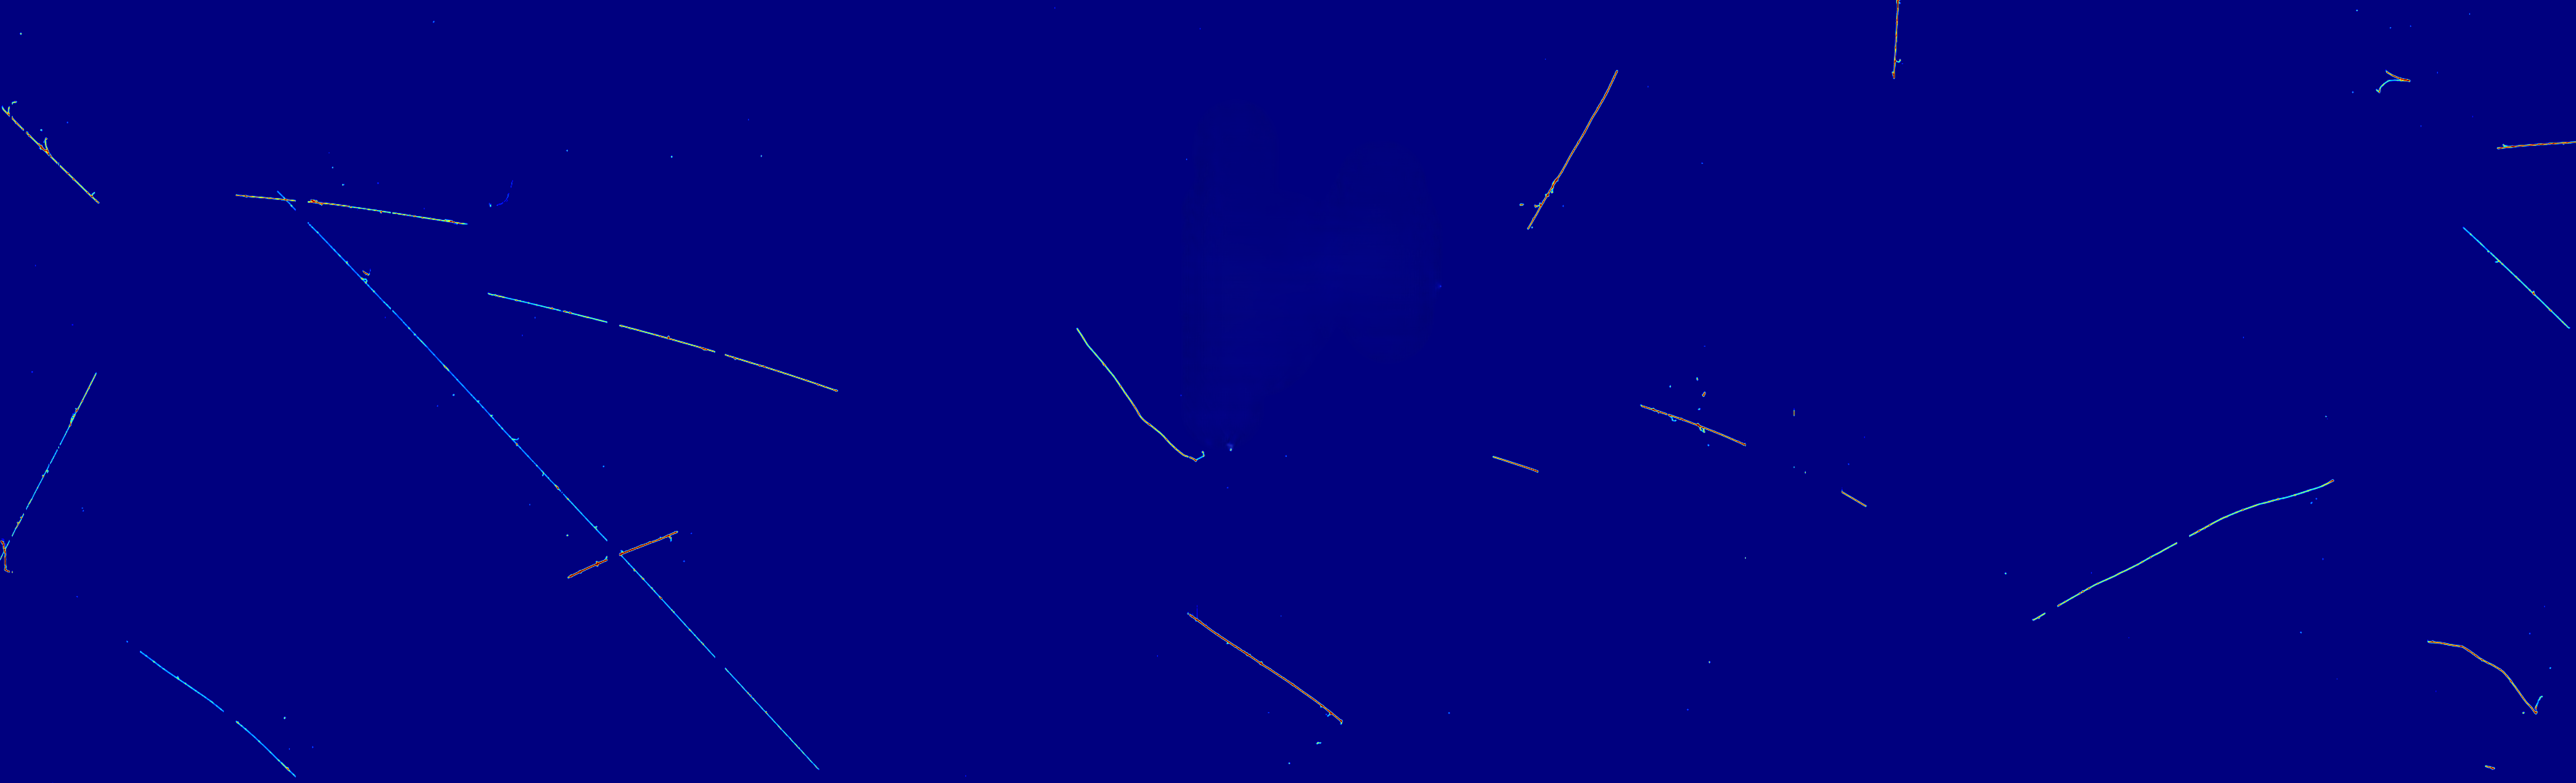
\includegraphics[width=0.9\textwidth]{src/wireimageIM.png}
    \caption{Example of noise patterns in lartcp detectors, taken from microBooNe \cite{ubooneOpenSamples}}
    \label{fig:noise}
\end{figure}

Neutrino interactions are not the only source of signals in the detector. Cosmic muons produced by secondary cosmic rays in the atmosphere can also ionize the detector medium, producing characteristic noise patterns. These patterns are typically distinct and easily distinguishable from genuine neutrino events. They often take the form of long, low-intensity tracks\ref{fig:noise}. The rate of such background events strongly depends on how deep the detector's been placed underground. DUNE's detector will be placed 1500m underground \cite{DUNE}, while MicroBooNE is located 6m underground \cite{MicroBooNEDesign}. One can therefore expect significantly fewer events from cosmic rays in signals from DUNE. However, complete elimination of these events is not possible. Therefore such events need to be accounted for and filtered out during data processing.

\chapter{MicroBooNE Experiment}

\section{Detector}

\begin{figure}[H]
    \centering
    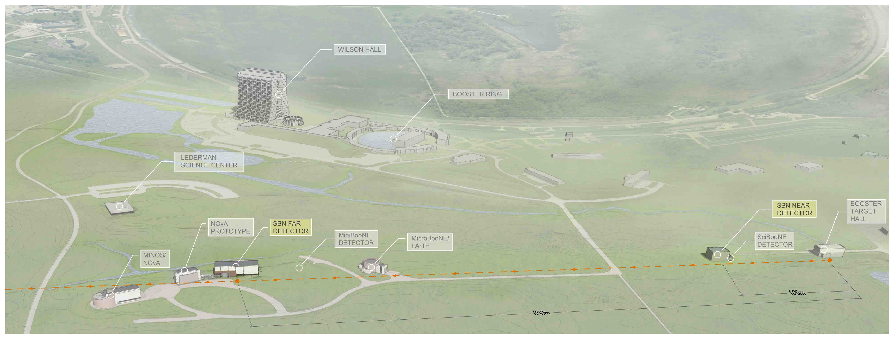
\includegraphics[width=0.80\textwidth]{src/microbooneBirdseyes.pdf}
    \caption{Aerial diagram showing location of MicroBooNE.\cite{MicroBooNEDesign}}
    \label{fig:microboone_birdseye}
\end{figure}

The MicroBooNE experiment began operation at Fermilab in 2015 and currently functions as the middle detector in the Short-Baseline Neutrino (SBN) program. Its primary scientific goal is to investigate the source of the excess of electron neutrino-like events observed in the predominantly muon neutrino beam by the MiniBooNE experiment. Its exact placement in the BNB (Booster Neutrino Beam), located 470~m from the neutrino source, is shown in Figure~\ref{fig:microboone_birdseye}. The BNB delivers neutrinos with energies in the range of 0.5–2~GeV.

MicroBooNE is based on a 170-ton liquid-argon TPC, enclosed in a cryostat and depicted in Figure~\ref{fig:microboone_layout}. Of this total argon mass, 89 tonnes form the active volume. Its general operating principle is strictly analogous to the one described by Figure~\ref{fig:lartcp}, with three sets of parallel wires serving the role of anode planes. The detector is located on the Fermilab site, as shown in Figure~\ref{fig:microboone_birdseye}. Key design parameters are summarized in Table~\ref{tab:microboone_specs}\cite{MicroBooNEDesign}.

In addition to its primary scientific goals, it contributes essential input toward the development of kiloton-scale liquid-argon time projection chambers (LArTPCs) for the upcoming Deep Underground Neutrino Experiment (DUNE).


\begin{table}[H]
\centering
\caption{Primary detector design parameters for MicroBooNE.\cite{MicroBooNEDesign}}
\begin{tabular}{|l|l|}
\hline
\textbf{Parameter} & \textbf{Value} \\
\hline
LArTPC Dimensions & 2.325 m vertically \\
                  & 2.560 m horizontally \\
                  & 10.368 m longitudinally \\
\hline
LArTPC argon mass & 90 tonnes \\
\hline
Total Number of Wires & 8256 \\
\hline
Drift field & 500 V/cm \\
\hline
Wire configuration & 3 anode wire planes \\
                   & 3 mm spacing between wires \\
                   & 3 mm spacing between planes \\
\hline
Total liquid argon mass & 170 tonnes \\
\hline
Operating temperature & 87 K \\
\hline
Depth & 6 m \\
\hline
\end{tabular}
\label{tab:microboone_specs}
\end{table}


\begin{figure}[H]
    \centering
    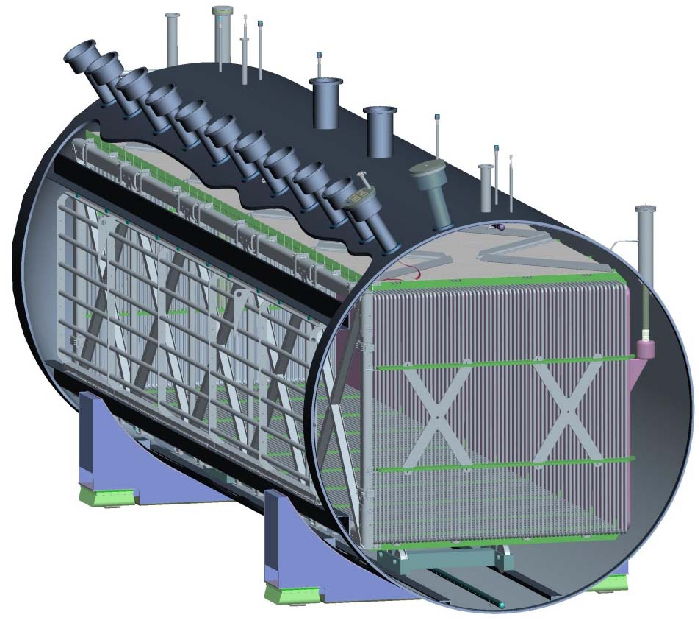
\includegraphics[width=0.65\textwidth]{src/microBooNe_Layout.pdf}
    \caption{Schematic diagram of the MicroBooNE LArTPC inside the cryostat.\cite{MicroBooNEDesign}}
    \label{fig:microboone_layout}
\end{figure}

\subsection{Publicly available datasets}

Two MicroBooNE datasets are opened to the public. They contain simulated neutrino interactions overlaid on top of cosmic ray data. These datasets were provided to support the development of new computational techniques for neutrino event reconstruction and analysis, primarily with DUNE in mind. They will be discussed in greater detail in the next chapter.

\chapter{MicroBooNE Public Datasets}

All the data used further in this work are two publicly available datasets from the MicroBooNE experiment: the Inclusive sample and the Electron Neutrino sample \cite{ubooneOpenSamples}. The Inclusive sample contains both charged-current (CC) and neutral-current (NC) interactions, as well as various neutrino types, reflecting the true composition of the Booster Neutrino Beam. The Electron Neutrino sample, on the other hand, contains only electron neutrino CC interactions.

The MicroBooNE OpenSamples dataset is provided in two formats: HDF5 and ROOT. The HDF5 format is a hierarchical data format suitable for efficient storage and access to large numerical datasets. The ROOT format is based on the ROOT framework, which is commonly used in high-energy physics for storing and analyzing complex event data structures~\cite{hdf5,root}. 

There are two main types of data samples: "with wires" and "no wires." The "with wires" datasets include full waveform data from the detector wires, allowing for signal reconstruction and image generation. The "no wires" datasets omit this raw waveform information and therefore do not allow for image reconstruction.

\section{Events Present}

\subsection{\texorpdfstring{$\nu_e$}{νₑ}-Enhanced Sample Description}

The distributions of lepton and neutrino energies for the two datasets are shown in Figures~\ref{fig:lepton-inclusive}--\ref{fig:neutrino-nue}. 

The $\nu_e$-enhanced sample consists of 19,940 events, containing a broader mix of neutrino types. The majority are muon neutrinos (23,984), followed by smaller numbers of muon antineutrinos (208 with PDG code $-14$), electron neutrinos (134 with PDG code 12), and electron antineutrinos (6 with PDG code $-12$). Of the total, 17,564 events are classified as charged-current (CC), while 6,768 are neutral-current (NC) interactions. Within the charged-current subset, 17,457 events originate from muon neutrinos or antineutrinos, and 107 from electron neutrinos or antineutrinos, indicating a dominance of muon neutrino interactions in this sample.

\begin{figure}[H]
    \centering
    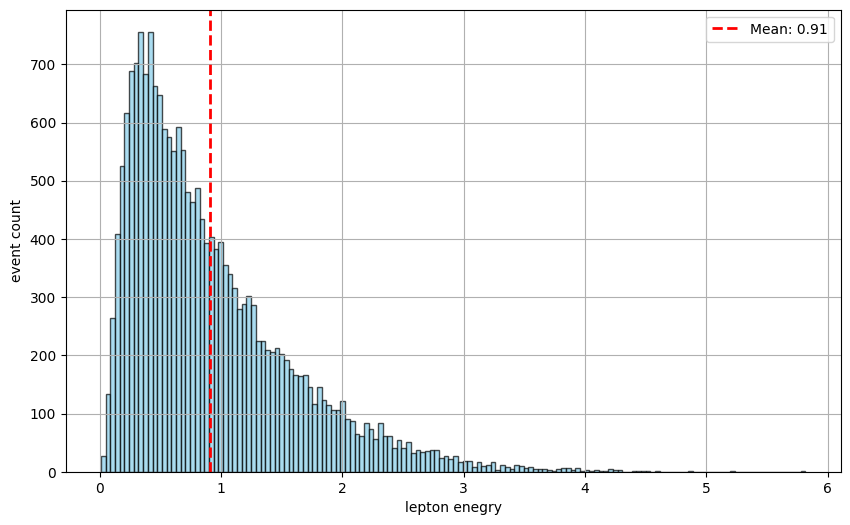
\includegraphics[width=0.75\textwidth]{src/leptonMuon.png}
    \caption{Lepton energy distribution in the Inclusive (BNB) sample. The vertical axis shows the number of events.}
    \label{fig:lepton-inclusive}
\end{figure}

\begin{figure}[H]
    \centering
    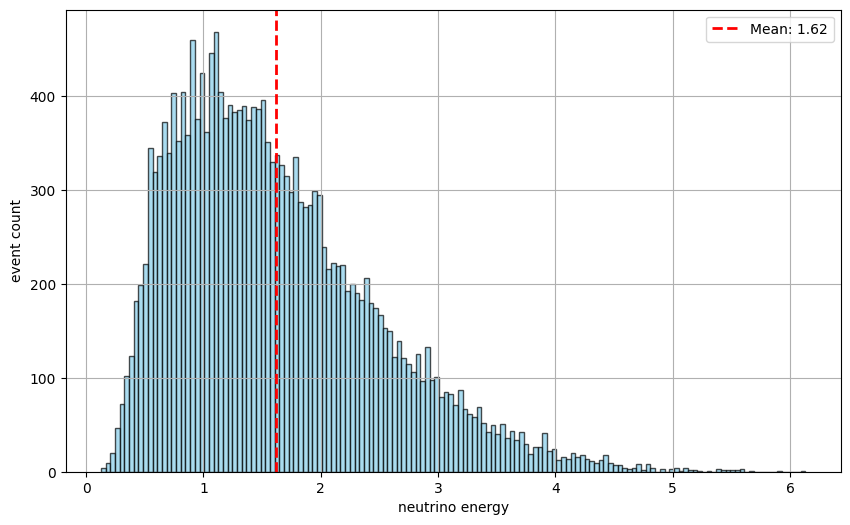
\includegraphics[width=0.75\textwidth]{src/neutrinoMuon.png}
    \caption{Neutrino energy distribution in the Inclusive (BNB) sample. The vertical axis shows the number of events.}
    \label{fig:neutrino-inclusive}
\end{figure}

The energy distribution of neutrino interactions in this sample has a mean value of 1.62~GeV, a median of 1.46~GeV, and a standard deviation of 0.86~GeV. The minimum recorded energy is 0.13~GeV, while the maximum reaches 6.13~GeV.

The associated charged lepton energy distribution exhibits a mean of 0.69~GeV, a median of 0.57~GeV, and a standard deviation of 0.50~GeV. The lepton energies range from 0.01~GeV to 5.67~GeV. These characteristics reflect a relatively high-energy subset of interactions, with lepton energy distributions concentrated in the sub-GeV to low-GeV range.

\subsection{BNB sample}

The distributions for the $\nu_e$-enhanced sample are shown in Figures~\ref{fig:lepton-nue} and~\ref{fig:neutrino-nue}.

The BNB (Booster Neutrino Beam, Inclusive) sample contains a total of 24,332 events, all of which are classified as charged-current (CC) interactions. The dataset is composed exclusively of electron neutrinos and antineutrinos, with 19,448 events corresponding to neutrinos (PDG code 12) and 492 to antineutrinos (PDG code $-12$). No muon neutrinos (PDG 14 or $-14$) are present.

\begin{figure}[H]
    \centering
    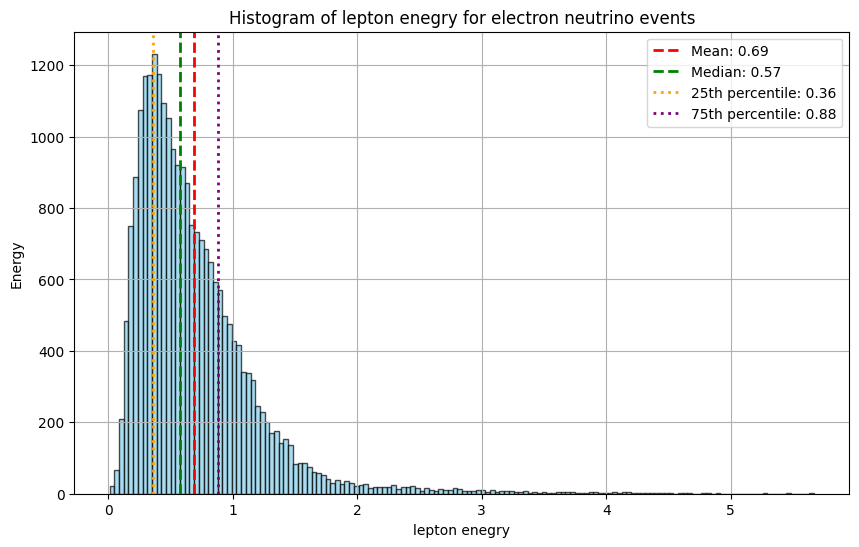
\includegraphics[width=0.75\textwidth]{src/leptonElectron.png}
    \caption{Lepton energy distribution in the nu\_e-enhanced sample. The vertical axis shows the number of events.}
    \label{fig:lepton-nue}
\end{figure}

\begin{figure}[H]
    \centering
    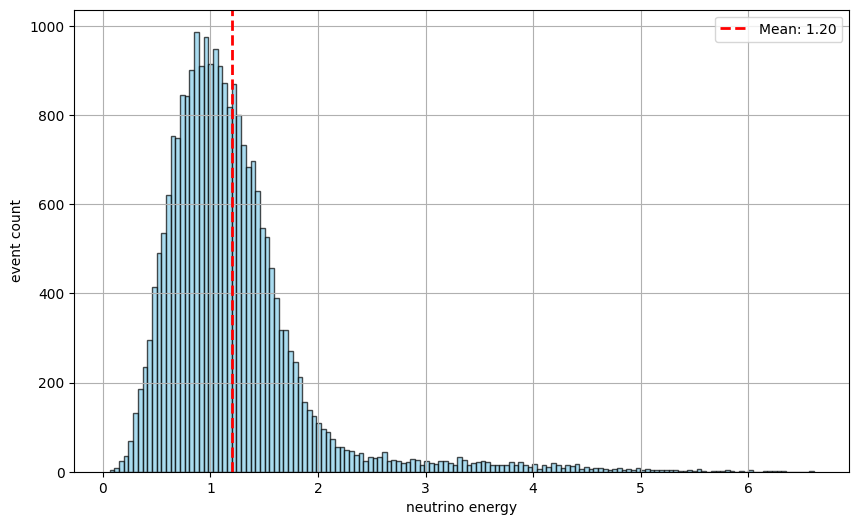
\includegraphics[width=0.75\textwidth]{src/neutrinoElectron.png}
    \caption{Neutrino energy distribution in the nu\_e-enhanced sample. The vertical axis shows the number of events.}
    \label{fig:neutrino-nue}
\end{figure}


The energy distribution shows a mean of 1.20~GeV, a median of 1.08~GeV, and a standard deviation of 0.67~GeV, with values ranging from 0.06~GeV to 6.61~GeV. The corresponding charged lepton energy distribution has a mean of 0.91~GeV, a median of 0.73~GeV, and a standard deviation of 0.67~GeV. Lepton energies range from 0.01~GeV to 5.82~GeV. This distribution suggests a slightly lower-energy spectrum on average, but with a broader mix of interaction types and moderate lepton energy variability.

\subsection{Combined Dataset}

The combined dataset consists of 44,272 events and includes a mix of neutrino interaction types. The dominant component is muon neutrinos (23,984), followed by electron neutrinos (19,582), electron antineutrinos (498), and a small number of muon antineutrinos (208). Out of the total, 37,504 events are classified as charged-current (CC) interactions, while 6,768 are neutral-current (NC). Within the CC category, 17,457 events originate from muon neutrinos or antineutrinos, and 20,047 from electron neutrinos or antineutrinos, indicating a more balanced representation of flavor types compared to the $\nu_e$-enhanced sample. 

\begin{table}[h]
\centering
\caption{Summary of Neutrino Events in the Dataset}
\begin{tabular}{|l|r|}
\hline
\textbf{Category} & \textbf{Count} \\
\hline
Total events & 44,272 \\
BNB sample & 24,332 \\
$\nu_e$-enhanced sample & 19,940 \\
\hline
\multicolumn{2}{|c|}{\textbf{In BNB sample}} \\
\hline
$\nu_{\mu}$ ($\text{PDG}=14$) & 23,984 \\
$\bar{\nu}_{\mu}$ ($\text{PDG}=-14$) & 208 \\
$\nu_e$ ($\text{PDG}=12$) & 134 \\
$\bar{\nu}_e$ ($\text{PDG}=-12$) & 6 \\
Charged current (CC) events & 17,564 \\
Neutral current (NC) events & 6,768 \\
CC $\nu_e$ or $\bar{\nu}_e$ events & 107 \\
CC $\nu_e$ events & 101 \\
CC $\nu_{\mu}$ or $\bar{\nu}_{\mu}$ events & 17,457 \\
CC $\nu_{\mu}$ events & 17,338 \\
Mean energy (GeV) & 1.20 \\
\hline
\multicolumn{2}{|c|}{\textbf{In $\nu_e$-enhanced sample}} \\
\hline
$\nu_e$ ($\text{PDG}=12$) & 19,448 \\
$\bar{\nu}_e$ ($\text{PDG}=-12$) & 492 \\
CC events & 19,940 \\
CC $\nu_e$ or $\bar{\nu}_e$ events & 19,940 \\
CC $\nu_e$ events & 19,448 \\
CC $\nu_{\mu}$ or $\bar{\nu}_{\mu}$ events & 0 \\
Mean energy (GeV) & 1.62 \\
\hline
\end{tabular}
\end{table}

\chapter{Dataset preparation}

The Jupyter notebooks accompanying the MicroBooNE OpenSamples repository recommend creating a Conda environment that includes the necessary packages. While there is nothing inherently wrong with this approach, it does introduce several disadvantages. Beyond general inefficiencies—such as longer environment loading times, higher memory usage, and increased disk space consumption—the most significant issue encountered was related to the sheer number of files generated by Conda distributions.

Both Conda and Miniconda installations can create and maintain hundreds of thousands of files. Although the total disk usage of these files is typically not problematic (many are symbolic links or small metadata files), the system used for processing data enforced strict quotas on the number of files each user could create. The data processing was performed on the ICM UW "Okeanos" cluster running CentOS 7. Installing a full Conda distribution brought the user account dangerously close to this limit, which severely impacted the usability of the system. For instance, launching a new Jupyter session became almost impossible, as nearly every action related to managing Jupyter generates additional log files, further pushing against the file quota.

Additionally, the environment setup proposed in the MicroBooNE OpenSamples notebooks depended on outdated libraries—most notably \texttt{pynuml} version 0.3, which is no longer maintained and is poorly documented. This package also requires an outdated version of Python (3.7) and depends on a deprecated version of HDF5. These constraints make it effectively impossible to use current versions of many essential packages, which significantly complicates the development process.

To address these issues and improve the portability and maintainability of the tools used for processing OpenSamples data, an alternative approach to environment management was adopted.

\subsection{Containerization and Singularity}

Containerization is a method of packaging software and its dependencies into isolated, self-contained units called containers. Each container includes all necessary binaries, libraries, and configuration files, ensuring that applications run consistently across different systems regardless of variations in the underlying infrastructure. Modern containerization solutions allow for building, distributing, and executing containers in a lightweight and reproducible manner. Containers are typically defined using a configuration file that builds on a base image and specifies additional dependencies and setup steps, producing a new image that can be versioned and reused.

In this specific case, a containerization tool called Singularity was used. Singularity is particularly well-suited for high-performance computing environments, as it enables users to define, build, and execute containers without requiring root privileges. A container definition file was created based on a Ubuntu 22.01 base image. (An image is a static, read-only template with the application and its dependencies, while a container is a running instance of an image, including its own filesystem and processes.) This definition specified the installation of all required dependencies and packages during the container build process. Using this approach made it possible to work with up-to-date software versions, including Python 3.9, pynuml version 25.4.0, and HDF5 version 1.12.2, although these upgrades required some code refactorings to be performed on the code present in OpenSamples notebooks. Moreover, since the resulting container image is stored as a single file, this method also effectively circumvented the file quota limitations encountered with Conda-based setups.


Containerization is a method of packaging software and its dependencies into isolated, self-contained units called containers. Each container includes all necessary binaries, libraries, and configuration files, ensuring that applications run consistently across different systems regardless of variations in the underlying infrastructure. Modern containerization solutions allow for building, distributing, and executing containers in a lightweight and reproducible manner. Containers are typically defined using a configuration file that builds on a base image and specifies additional dependencies and setup steps, producing a new image that can be versioned and reused.

The definition files for containers used to produce results presented in this work can be found in the repository listed in the appendix.


\subsection{HDF5 File Structure}

Data stored in HDF5 files was separated into multiple tables, each containing a specific type of information. The tables are organized hierarchically, with the root directory containing the main event table and additional subdirectories for other data types. Each table is structured as a collection of records, where each record corresponds to a single event or hit in the detector. The tables are designed to be self-describing, meaning that they include metadata about the data types and structures used within them.
The HDF5 file structure for the MicroBooNE OpenSamples dataset contains multiple tables with specific information types. A detailed description of all tables is provided in Appendix~\ref{app:hdf5_structure}.

Because of their smaller size, HDF5 files were used for the initial data extraction. Although the HDF5 format is well-suited for storing large datasets, reading from it can require loading substantial portions of data into memory—a time-consuming operation that makes it impractical to use these files directly for neural network training. Therefore, a decision was made to extract the relevant data and store it in a simpler, more accessible format.

The final extracted dataset consisted of a CSV file containing the composite event ID (run number, subrun number, and event number), neutrino energy, and the \texttt{is\_cc} value from the event table, as well as the \texttt{PDG} of the interacting neutrino. Another file matching the same composite ID with the lepton energy was also created. These were later joined during processing. Additionally, it included the filenames of three image files, each corresponding to one of the three wire planes. These images were generated from the wire readouts and represent visualizations of the recorded signals.

\subsection{Data extraction}

Data from the \texttt{wire\_table}, \texttt{edep\_table}, and \texttt{lep\_table} was first matched with corresponding events in the \texttt{event\_table} (this was largely based on the code present in the Wireimage.ipynb notebook provided by the authors of the dataset). From each matched record, the lepton energy was extracted from the \texttt{lep\_table}, the neutrino energy from the \texttt{edep\_table}, and the \texttt{is\_cc} value from the \texttt{event\_table}. The \texttt{wire\_table} was used to obtain the wire signals for each event. It was subsequently processed into images, and linked to the corresponding event metadata for downstream analysis.

\section{Image Rendering}

\begin{figure}[H]
    \centering
    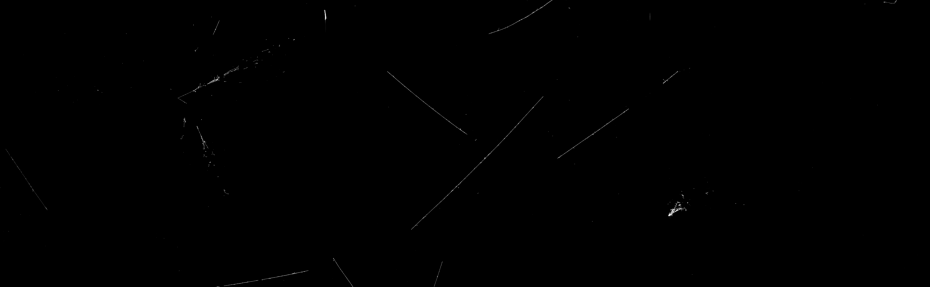
\includegraphics[width=0.8\textwidth]{src/with_flag_58.png}
    \caption{Example of a wire readout image}
\end{figure}

Images were generated using data from the wire readouts, where the horizontal axis corresponds to the wire number and the vertical axis to time. Each pixel represents the signal recorded on a specific wire at a given time. To suppress noise, a threshold was applied, below which wire activity was not visualized. Additionally, a saturation limit was introduced to prevent high-intensity signals from dominating the image. Pixel intensities were linearly scaled to an 8-bit range (0--255), and the resulting images were downsampled by a factor of two to reduce dataset size. This procedure was applied to all three wire planes, producing three images per event. These images were later saved as PNG files, and their filenames were stored in an appropriate CSV manifest file (a summary file listing all images and their associated metadata for each event).

\subsection{Final Dataset}

The final dataset consisted 132,816 PNG images, each representing a wire readout from the MicroBooNE detector alongside 38 CSV manifest files, each representing events form a single HDF5 file. This dataset turned out to contain approximately 13~GB of data, with each image file averaging around 100~KB in size.

\section{Further Dataset Processing}

\subsection{Sparse array representation}

\begin{figure}[H]
    \centering
    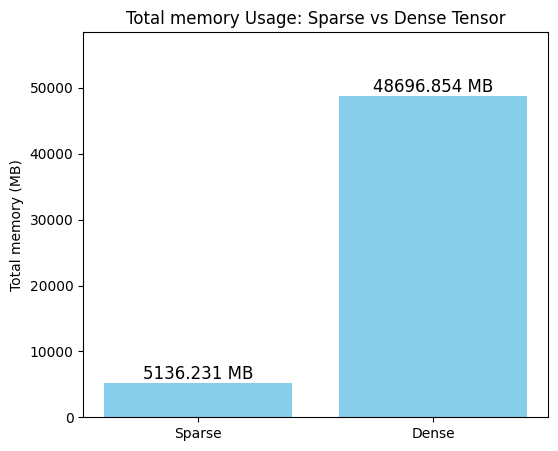
\includegraphics[width=0.55\textwidth]{src/totalSparseDense.png}
    \caption{Comparison of total memory usage between dense and sparse array representations.}
    \label{fig:memRedTot}
\end{figure}


Although the final image dataset occupied approximately 13~GB on disk, this was primarily due to the use of compressed image formats (specifically, PNG). When these images were loaded into memory as arrays of integers, their size increased dramatically—by more than a factor of 100 in some cases. It quickly became evident that the dataset was too large to be feasibly loaded into the system's RAM without causing memory fragmentation. However, loading each image individually into memory incurred significant computational overhead: each image had to be read from disk, memory had to be allocated, and the image had to be decompressed before being converted into an array. Since training a convolutional neural network (CNN) typically requires each image to be loaded multiple times, it was crucial to minimize the number of image loading operations.

\begin{figure}[H]
    \centering
    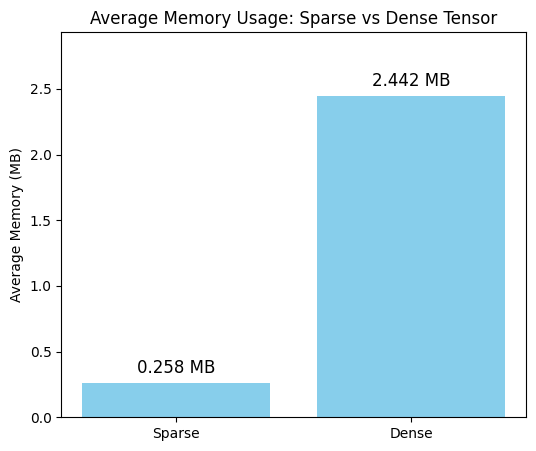
\includegraphics[width=0.55\textwidth]{src/sparseDenseComp.png}
    \caption{Comparison of average memory usage between dense and sparse array representations.}
    \label{fig:memRedAvg}
\end{figure}

During development, it was observed that the processed images contained mostly empty (zero-value) pixels. While tracks were present in all images, they typically occupied only a small portion of each image—approximately 5\% of the total pixels. (Note: Mention that the threshold used during the generation of wire images was sufficiently low to eliminate noise.) As a result, the decision was made to represent the images using sparse arrays (implemented with \texttt{torch.sparse}) Unlike dense arrays, where each element is stored explicitly in memory, sparse arrays assume a default value for all positions and store only the non-zero values along with their coordinates. Although these sparse arrays still need to be converted to dense format before being passed to the CNN, this conversion is significantly less costly than loading and decompressing images from disk. This optimization led to a substantial reduction in memory usage—by up to a factor of 70—making it feasible to load the entire dataset into RAM. The magnitude of those size reductions are shown in Figures~\ref{fig:memRedTot} and~\ref{fig:memRedAvg}.
\subsection{File count reduction}

The final dataset contained a significant amount of files - namely approximately 120,000 image files. This created issues similar to those previously encountered when working with Miniconda—namely, the operaing system configurations used on ICM rysy and topola clusters used for CNN training imposed quotas on the number of files each user could allocate. Operating under an account close to that limit proved to be cumbersome. Notably, the total dataset size remained well below the storage quota in terms of bytes, indicating that reducing the number of files could resolve the problem without affecting overall storage usage.

To address both issues, each CSV file was loaded into a pandas DataFrame. Three additional columns were added to each record—one for each image associated with an event—and populated with the corresponding sparse arrays. Each resulting dataset was then saved as a single \texttt{.pkl} file, a format that preserves Python objects as they exist in memory. In total, 38 .pkl files were created, each corresponding to one original HDF5 file and containing all events and associated images from that file. The combined size of all \texttt{.pkl} files was approximately 32~GB, which corresponds closely to the amount of memory required to load them into RAM.

\chapter{Classification Task definition}

\begin{figure}[H]
\centering

\includegraphics[width=0.8\textwidth]{src/electronShower.pdf}
\caption{Example of an electromagnetic shower produced by an electron neutrino interaction in a LArTPC detector (marked in red).}
\label{fig:electron_shower}
\end{figure}

\begin{table}[H]
    \centering
    \caption{Summary statistics of the full and \texttt{top50} datasets used for classification.}
    \label{tab:dataset_stats}
    \begin{tabular}{lccc}
        \toprule
        \textbf{Dataset} & \textbf{Total No. of Events} & \textbf{Background} & \textbf{Signal $\mu_e$ } \\
        \midrule
        Full Dataset     & 44,272                 & 24,225 & 20,047 \\
        \texttt{top50} Dataset & 22,136                 & 10,739 & 11,397 \\
        \bottomrule
    \end{tabular}
\end{table}

A general heuristic can be assumed: the more significant the visual difference between two classes in a classification problem, the better an image classification algorithm will perform. However, the problem should remain non-trivial and possess potential scientific utility.

As mentioned before, charged current neutrino interactions produce leptons. The different types of leptons resulting from these interactions can be distinguished. When passing through a LArTPC chamber, electrons—produced in electron neutrino interactions—generate electromagnetic showers. These showers are highly visible and have a very distinguishable shape (they appear as 'showers', not tracks), making them easily identifiable \ref{fig:electron_shower}.

The dataset was therefore divided based on whether or not a charged current electron neutrino interaction occurred in a given sample.

To simplify the problem further (by narrowing the data down to interactions with the most pronounced electron showers), an additional dataset was created. This subset contains only the 50\% most energetic electron neutrino charged current interactions. The size of the other class was also reduced arbitrarily to avoid class imbalance. This dataset is further referred to in the work as \texttt{top50}.

All the machine learning models discussed further in this work were trained on these aforementioned classification tasks. A summary of the number of members of each class for each dataset can be found in Table \ref{tab:dataset_stats}. For simplicity, every network in this work was trained only on images created based on the wire readouts from the plane 2.

\chapter{Machine learning fundamentals}

All information from this section was taken from \cite{MlBasics}.

Machine learning algorithms aim to find a mapping from a specific set of points in an input space to a corresponding set of points in an output space, both of which are predefined. These algorithms define a procedure for learning such a mapping based on a given set of input-output pairs, commonly referred to as the training data. Once learned, this mapping can be applied to all points in the input space, including those not included in the training set. The general expectation is that the mapping learned from the training data will generalize well to previously unseen data, enabling the algorithm to make accurate predictions or classifications on new inputs.

\section{Supervised machine learning}

The problems tackled in this work are classification problems, where the input space consists of images of wire readouts, and the output space consists of a binary label. The common way of tackling such problems is supervised machine learning.
In supervised machine learning, the training data is given in the form of input-target pairs \( \{(\mathbf{x}_i, y_i)\}_{i=1}^N \), where \( \mathbf{x}_i \in \mathbb{R}^d \) represents the feature vector of the \( i \)-th input and \( y_i \in \mathcal{Y} \) is the corresponding target value. The aim is to learn a function \( f: \mathbb{R}^d \rightarrow \mathcal{Y} \) that approximates the true relationship between inputs and outputs.

The central objective is to find a function \( f \) such that:
\[
f(\mathbf{x}_i) \approx y_i \quad \forall i \in \{1, \dots, N\}
\]

\section{Machine Learning Models}

\subsection{ML model definition and learnable Parameters}

The term machine learning model mentioned further in the work will refer to a pairing of a set of learnable parameters \( \boldsymbol{\theta} \in \mathbb{R}^p \), where \( p \) is the total number of parameters, and a model function \( f(\mathbf{x}; \boldsymbol{\theta}) \) which maps the input space to the output space. The learnable parameters \( \boldsymbol{\theta} \) are variables within the model that can be adjusted during the training process to minimize the difference between the model's predictions and the actual target values. They have a direct influence on the model's output.


The training process begins by setting all elements of \( \boldsymbol{\theta} \) with some initial values. For each training iteration, a batch of input data \( \mathbf{X} \in \mathbb{R}^{b \times d} \) is passed through the model, and the corresponding predictions \( \hat{\mathbf{y}} \in \mathbb{R}^b \) are obtained:

\[
\hat{\mathbf{y}} = f(\mathbf{X}; \boldsymbol{\theta})
\]

These predictions are then compared to the true labels \( \mathbf{y} \in \mathbb{R}^b \), and the parameters \( \boldsymbol{\theta} \) are updated to reduce the discrepancy. This step is repeated iteratively, refining \( \boldsymbol{\theta} \) over time to improve predictive performance. Each such update constitutes a learning step, and the entire iterative process is referred to as model training.

\subsection{Neural networks}

\begin{figure}[H]
\centering
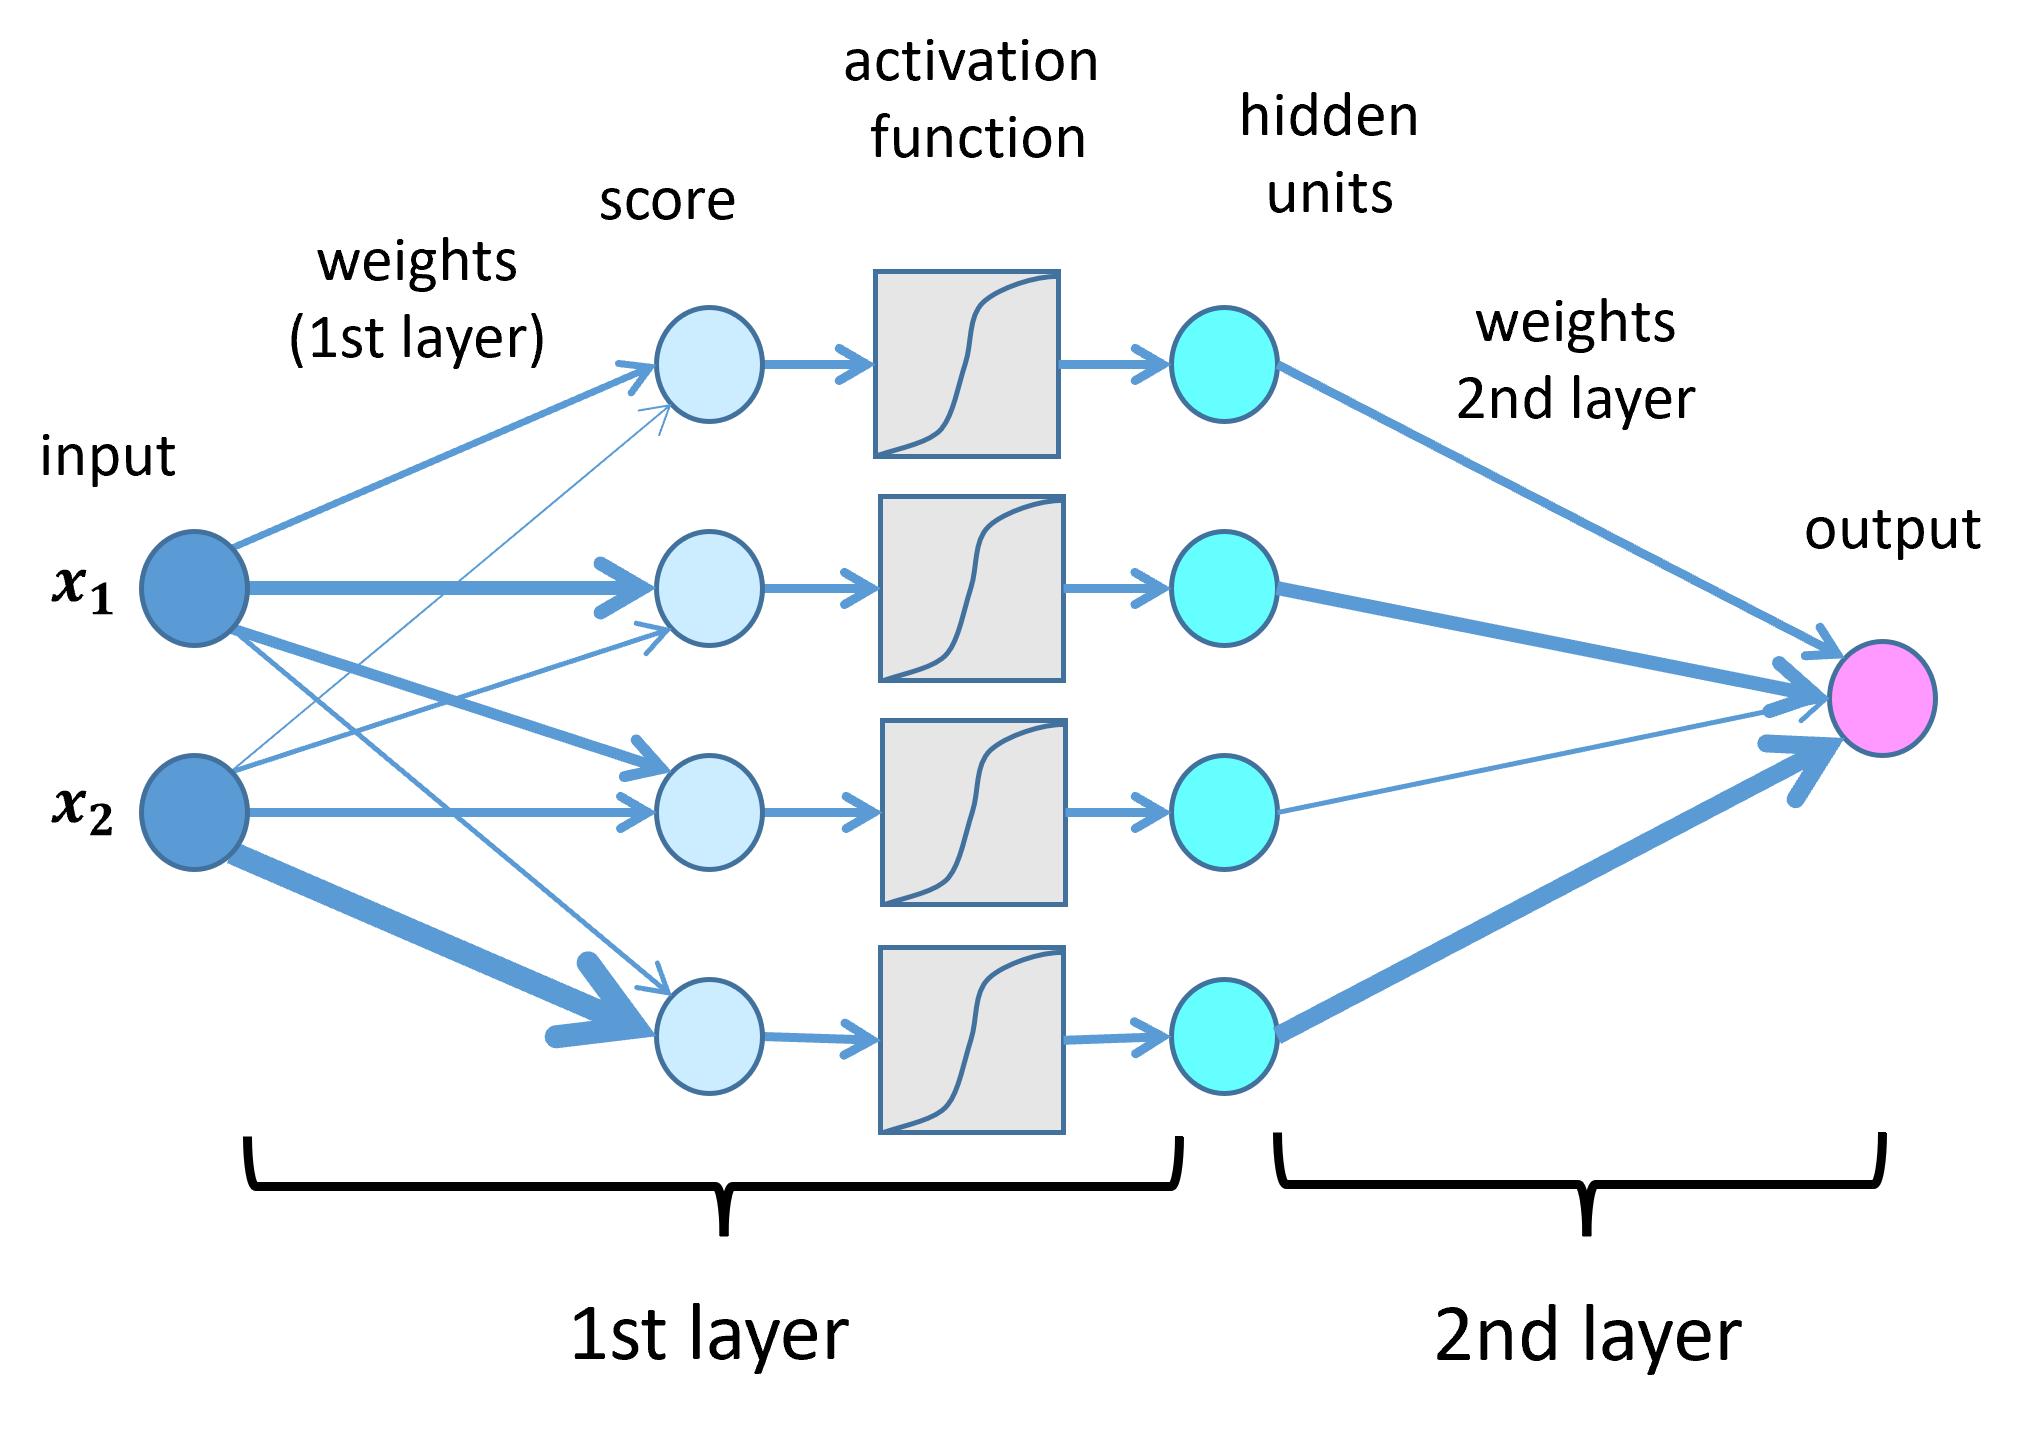
\includegraphics[width=0.7\textwidth]{src/deepNet.png}
\caption{Visualization of a neural network \cite{deepLearningRoundup2025}}
\label{fig:deepN}
\end{figure}

Neural networks are a class of machine learning models inspired by the structure of biological neurons. They consist of layers of interconnected nodes, also known as neurons, where each node computes a weighted sum of its inputs followed by a non-linear transformation. These networks are particularly effective for learning high-dimensional patterns in data, especially in tasks such as image recognition, classification, and regression.

A typical neural network consists of an input layer, one or more hidden layers, and an output layer \ref{fig:deepN}. Each layer performs a transformation of the form:

\[
\mathbf{h}^{(l)} = g^{(l)}(\mathbf{W}^{(l)} \mathbf{h}^{(l-1)} + \mathbf{b}^{(l)})
\]

where \( \mathbf{W}^{(l)} \) and \( \mathbf{b}^{(l)} \) are the learnable weights and biases of layer \( l \), \( g^{(l)} \) is a non-linear activation function, and \( \mathbf{h}^{(l-1)} \) is the output of the previous layer.

\subsubsection{Activation Functions}

Activation functions introduce non-linearity into the model, allowing the network to learn complex and non-linear decision boundaries. Two activation functions are used in the models discussed in this work: ReLU and Softmax.

\paragraph{ReLU}

The Rectified Linear Unit (ReLU) is a widely used activation function defined as:

\[
g(x) = \max(0, x)
\]

\begin{figure}[H]
\centering
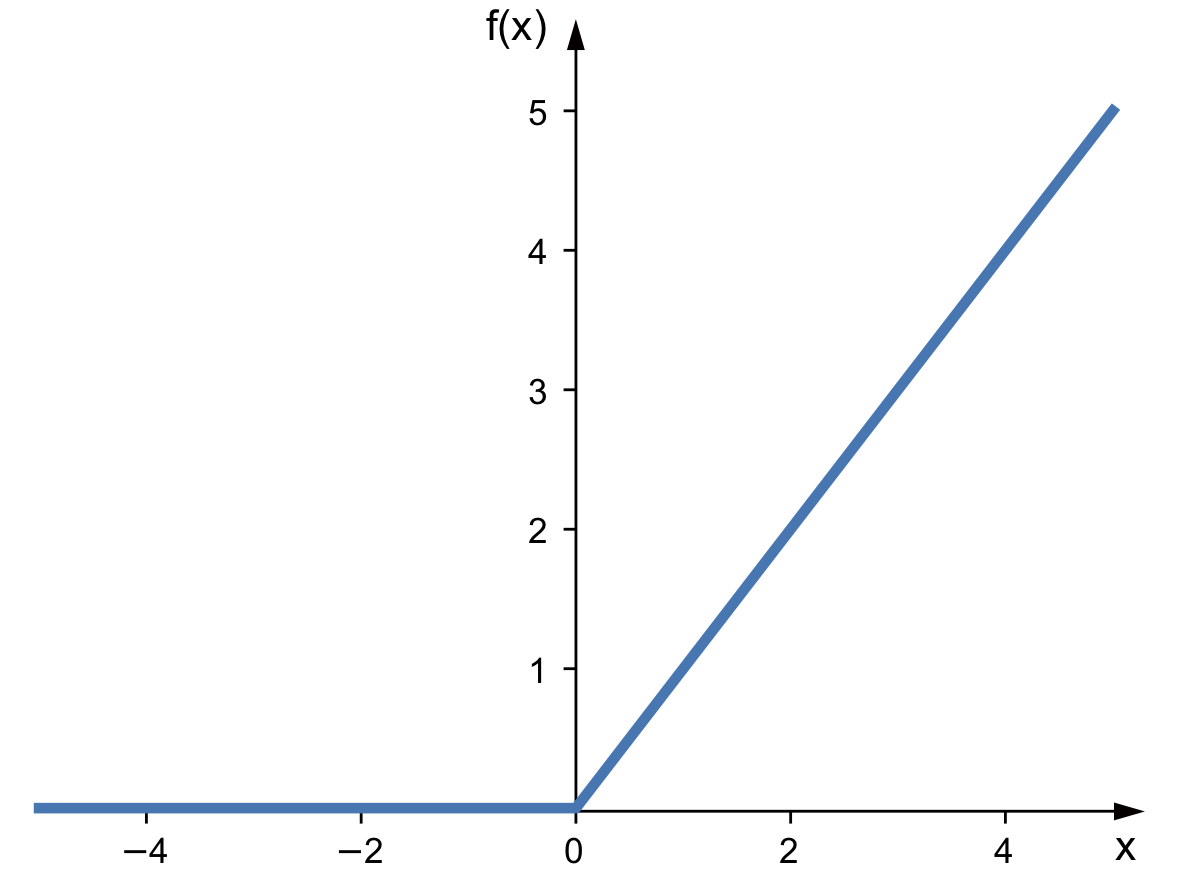
\includegraphics[width=0.5\textwidth]{src/relu.png}
\caption{Graph of the ReLU activation function.\cite{raschkaRelu}}
\label{fig:relu}
\end{figure}

Example plot of such function is shown in figure~\ref{fig:relu}.

\paragraph{Softmax}

\begin{figure}[H]
\centering
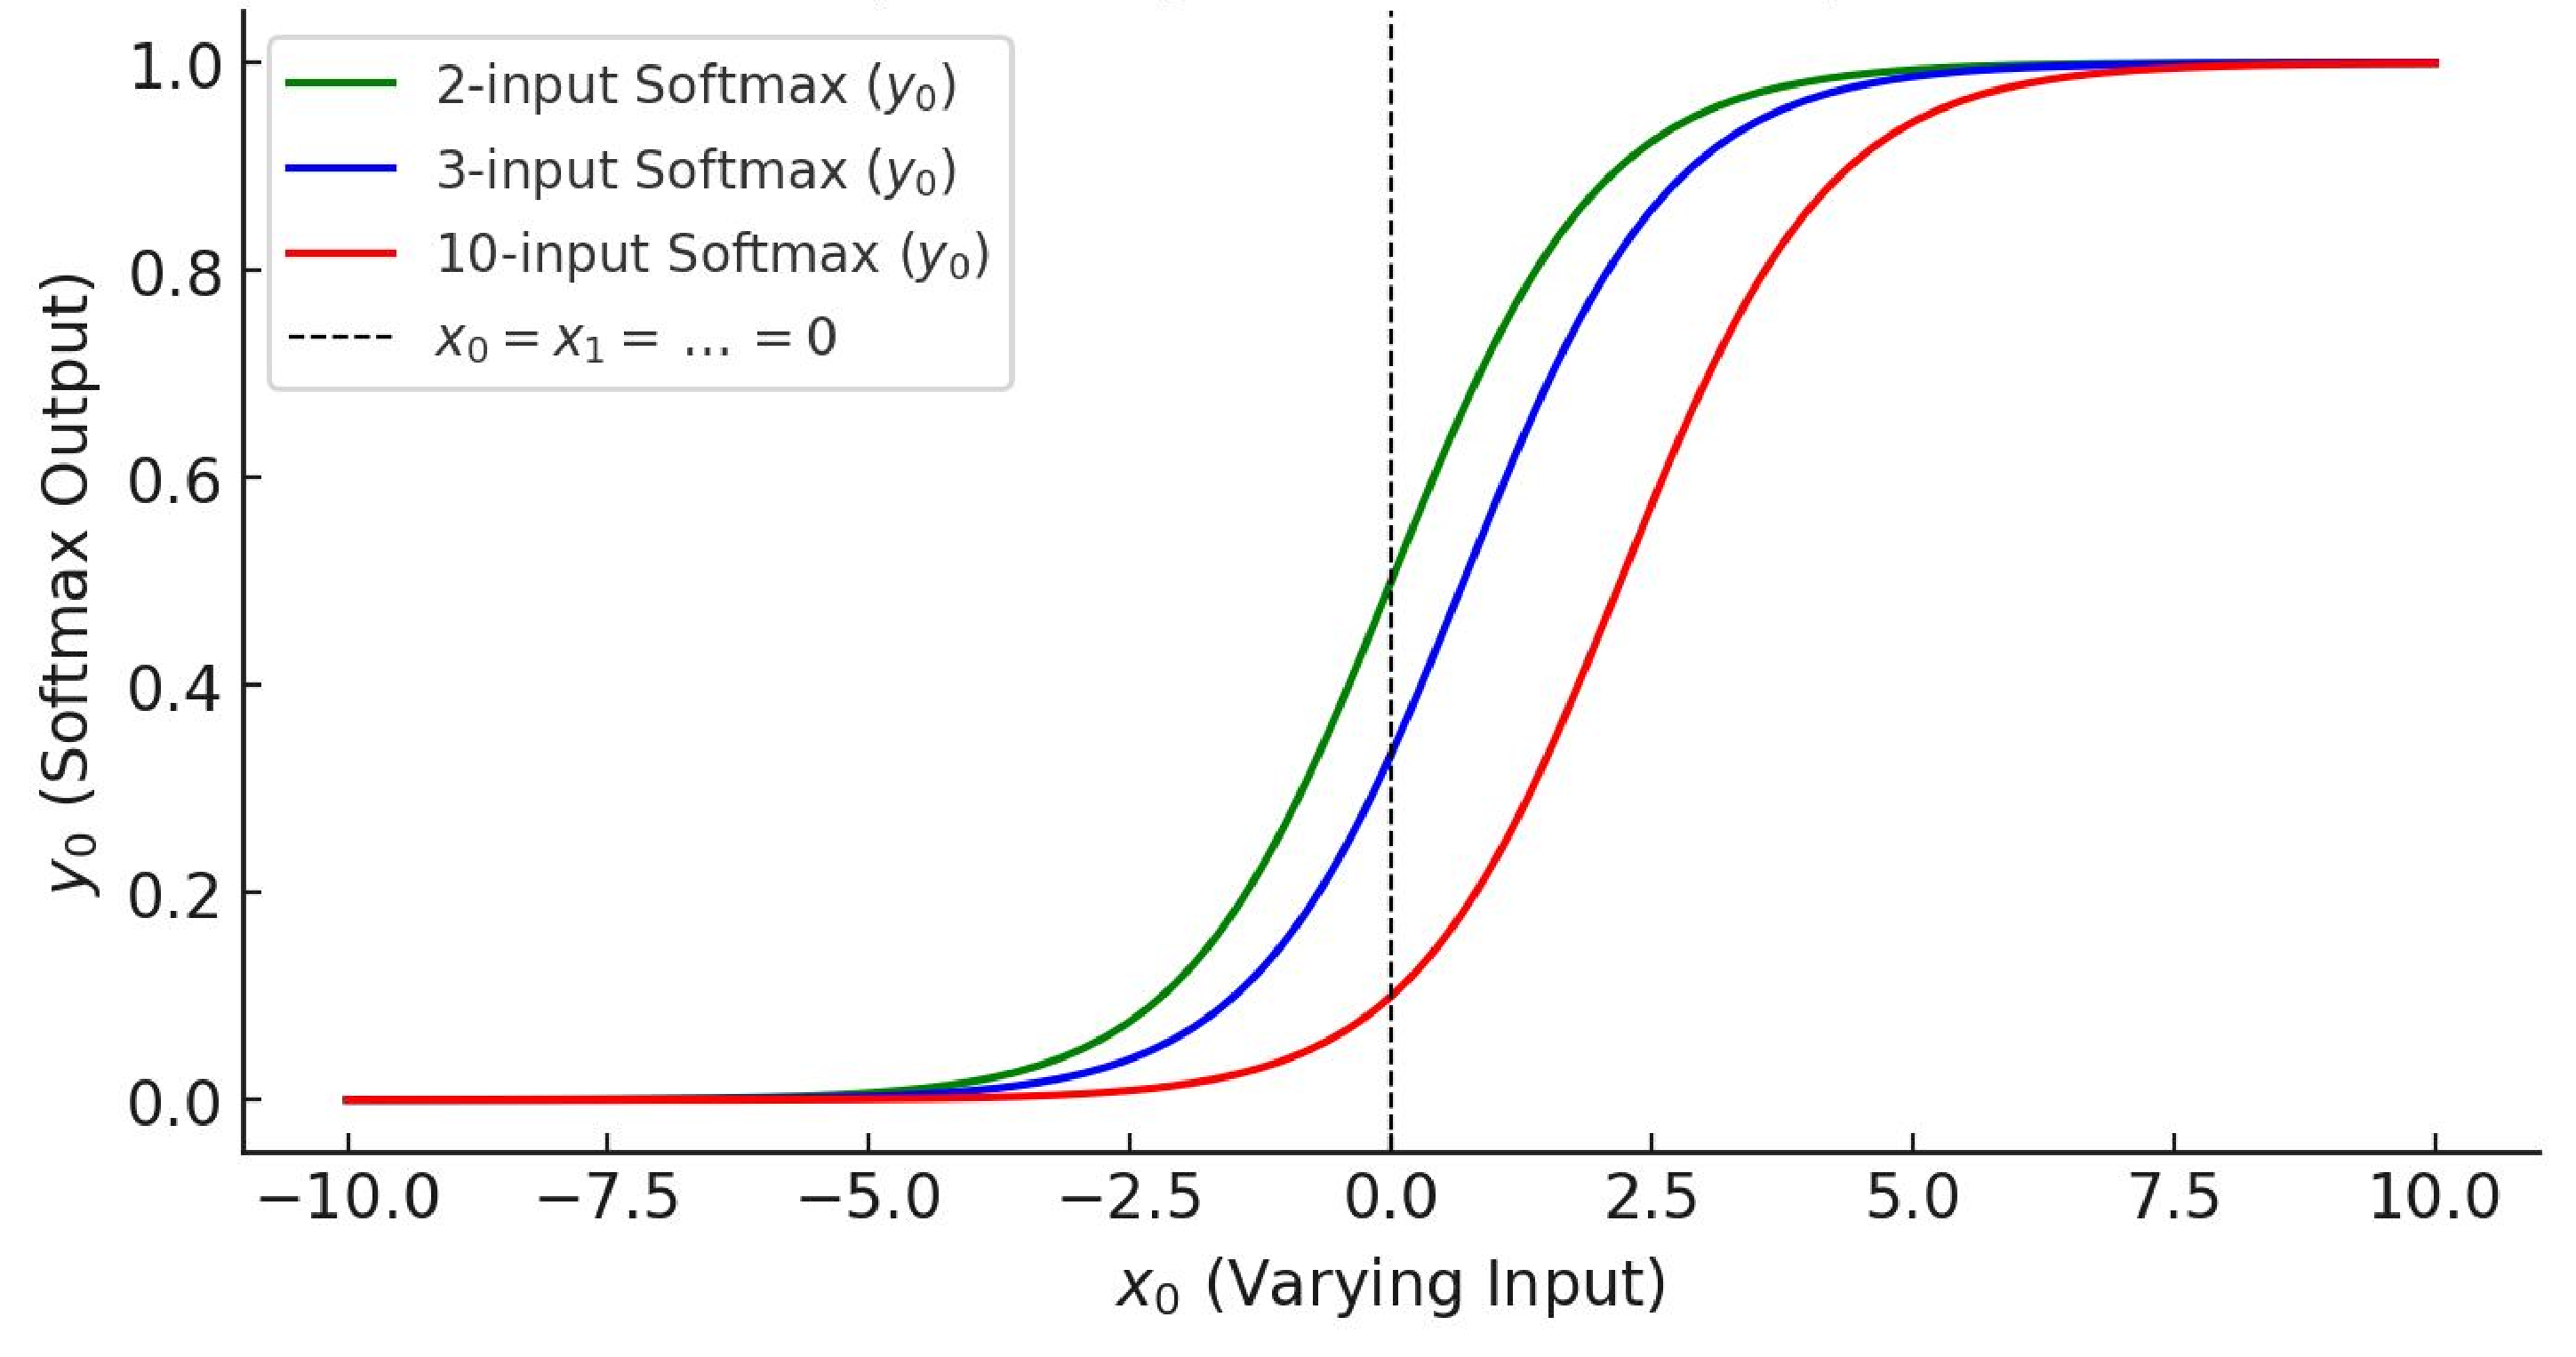
\includegraphics[width=0.55\textwidth]{src/softmax.pdf}
\caption{Softmax output $y_0$ as a function of input $x_0$, with all other inputs fixed at zero ($x_1 = x_2 = \ldots = 0$), for different numbers of total inputs: 2, 3, and 10 \cite{softmaxRef}.}
\label{fig:softmax}
\end{figure}

The Softmax function is used in the output layer of classification networks to convert raw output scores into a normalized probability distribution over \( C \) classes:

\[
\sigma(\mathbf{z})_i = \frac{e^{z_i}}{\sum_{j=1}^{C} e^{z_j}} \quad \text{for } i = 1, \dots, C
\]

This property makes it well-suited for multi-class classification tasks, where each input must be assigned a single label. It's general behaviour can be seen in figure~\ref{fig:softmax}.

\subsection{Loss Function}

The quality of the model's predictions is assessed using a loss function 

\[
\mathcal{L}(\hat{y}, y)
\]

Here $y$ stands for the true target value, while \( \hat{y} = f(\mathbf{x}; \boldsymbol{\theta}) \) is the model's prediction for a given input \( \mathbf{x} \).

The role of this function is to quantify the difference between predicted and true outputs. By assumtion the value of the loss function is non-negative, with lower values indicating better model performance (the outputs of the model are given ).

The choice of an optimal loss function is problem-specific but, regardless of the choice, the goal is to minimize the loss function with respect to the model parameters:

\[
\min_{\boldsymbol{\theta}} \ \mathcal{L}(f(\mathbf{x}; \boldsymbol{\theta}), y)
\]

\subsubsection{Cross-Entropy Loss}

Because of the nature of the problems discussed in this work, the cross-entropy loss function was used. This loss function is commonly applied to classification tasks.

The function in question measures the dissimilarity between the predicted probability distribution \( \hat{\mathbf{y}} \) over classes and the true class label distribution \( \mathbf{y} \), typically represented as a \textit{one-hot encoded vector}—a binary vector of length \( C \), where all entries are zero except for a one at the index corresponding to the correct class. For a single example and \( C \) classes, the cross-entropy loss is defined as:
\[
\mathcal{L}_{\text{CE}}(\mathbf{y}, \hat{\mathbf{y}}) = -\sum_{i=1}^{C} y_i \log(\hat{y}_i)
\]

This loss penalizes incorrect confident predictions more heavily and encourages the model to assign high probability to the correct class. Minimizing the cross-entropy therefore drives the model to output probability distributions that closely align with the true labels.

\subsection{Gradient Descent Optimization}

\begin{figure}[H]
    \centering
    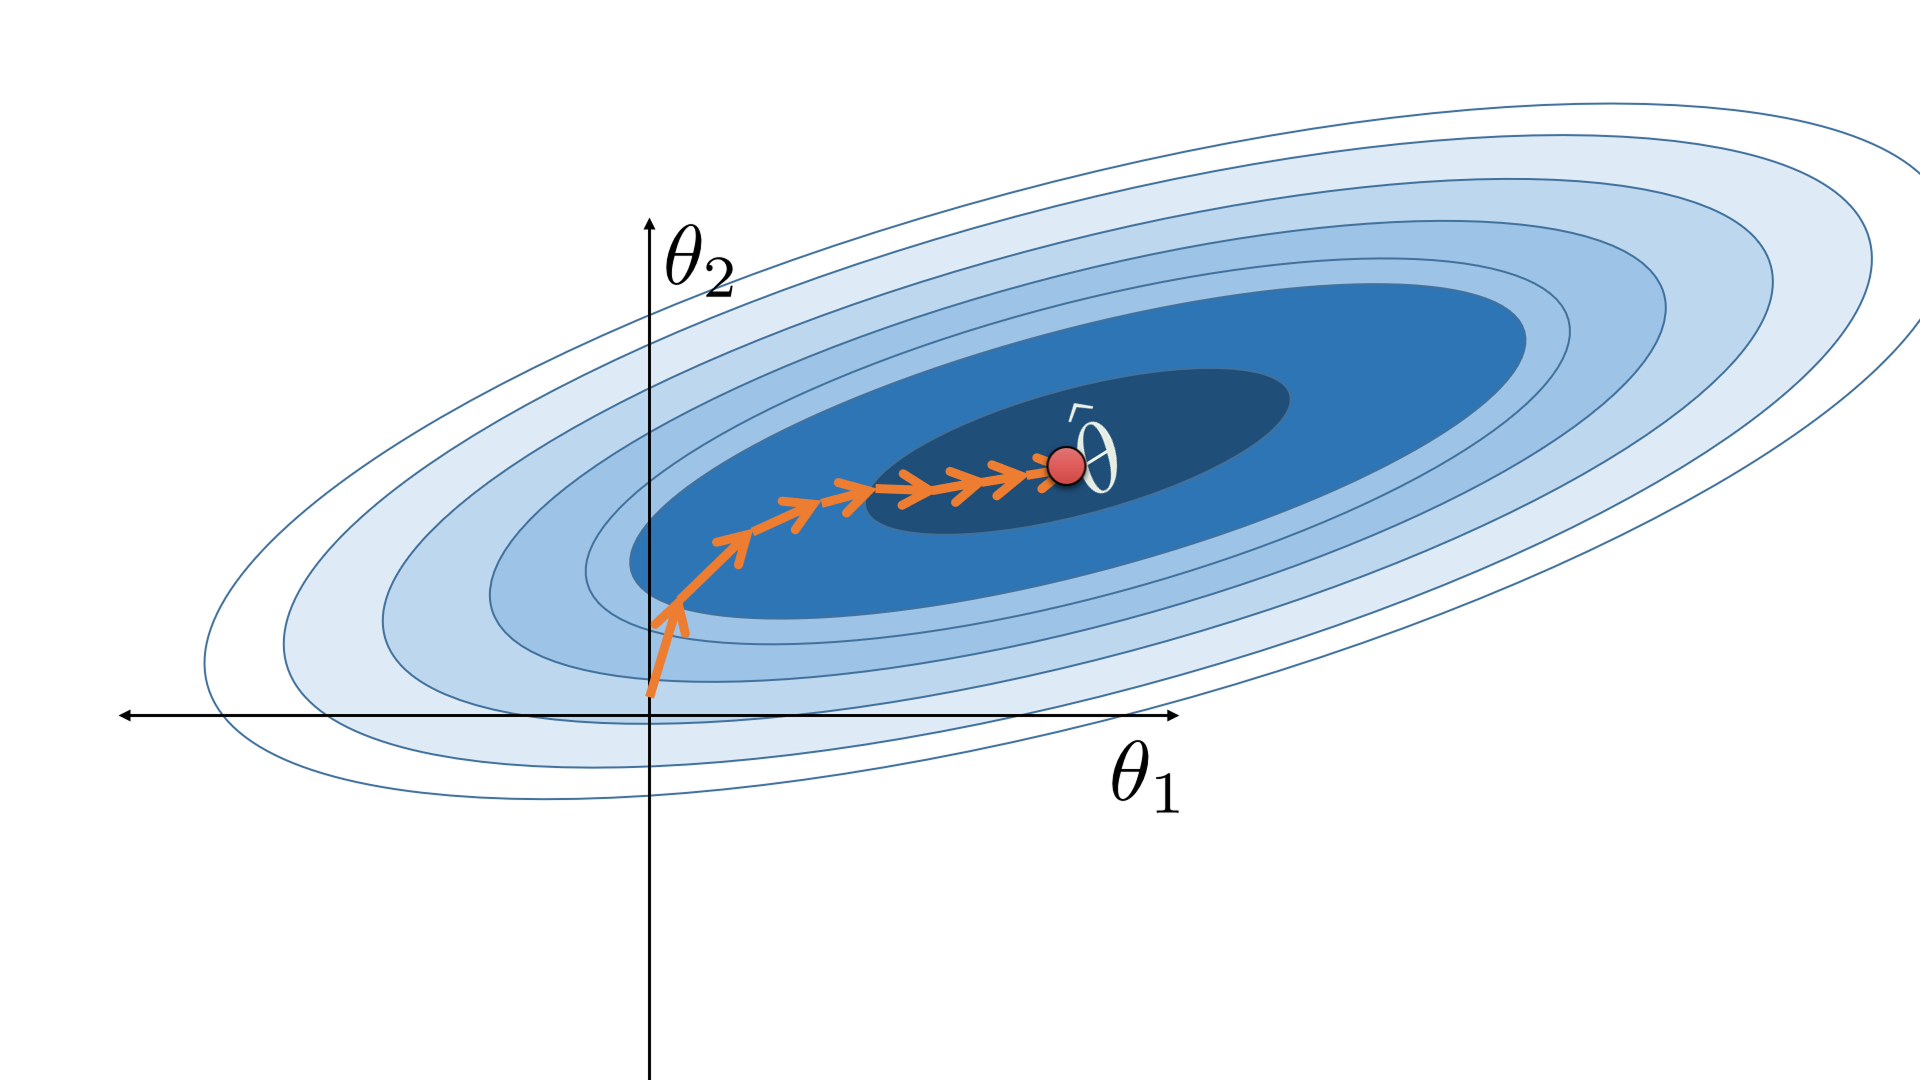
\includegraphics[width=0.75\textwidth]{src/gradienDescent.png}
    \caption{Gradient descent visualization. A local minimum is achieved by taking steps of a predefined size in the direction of the steepest descent\cite{Lau2023LearningDS}.}
\end{figure}

The approach used for training models used in this work is called \textit{gradient descent}. In particular, stochastic gradient descent (SGD). In each iteration, the gradient of the loss function with respect to the model parameters is computed:

\[
\nabla_{\boldsymbol{\theta}} \mathcal{L} = \left[ \frac{\partial \mathcal{L}}{\partial \theta_1}, \frac{\partial \mathcal{L}}{\partial \theta_2}, \dots, \frac{\partial \mathcal{L}}{\partial \theta_p} \right]^\top
\]

This gradient vector indicates the direction in parameter space that increases the loss most steeply. The parameters are then updated in the opposite direction of the gradient to reduce the loss:

\[
\boldsymbol{\theta} \leftarrow \boldsymbol{\theta} - \eta \nabla_{\boldsymbol{\theta}} \mathcal{L}
\]
where \( \eta > 0 \) is the learning rate, a hyperparameter that controls the step size.

By repeating this process over multiple iterations and batches of training data, the parameters ideally converge to a local minimum of the loss function. At convergence, the model's predictions are as close as possible to the target values within the expressiveness of the chosen architecture.

This iterative process of computing gradients and updating parameters is known as \textit{gradient descent}.

\subsubsection{Momentum}

In order to smooth out the gradient descent and accelerate convergence a \textit{momentum} can be introduced to a sdg algorithm. When introduced the descent direction incorporates a fraction of the previous update step, instead of relying solely on the current gradient.

The momentum update rule is defined as:

\[
\begin{aligned}
\mathbf{v}_t &= \gamma \mathbf{v}_{t-1} + \eta \nabla_{\boldsymbol{\theta}} \mathcal{L}(\boldsymbol{\theta}_{t-1}) \\
\boldsymbol{\theta}_t &= \boldsymbol{\theta}_{t-1} - \mathbf{v}_t
\end{aligned}
\]

Here, \( \mathbf{v}_t \) is the velocity vector (accumulated update), \( \gamma \in [0,1) \) is the momentum coefficient, and \( \eta \) is the learning rate. A higher \( \gamma \) allows more influence from previous gradients, leading to smoother and potentially faster convergence.

\subsection{Output Layer and Thresholding}

In binary classification tasks, the output layer of the neural network perceptron contains two neurons, each representing one of the two possible classes. The network produces a pair of output values, which are interpreted as unnormalized logit scores (i.e., the raw, unscaled values output). These scores are typically passed through a softmax function to produce a probability distribution over the two classes:

\[
\hat{y}_i = \frac{e^{z_i}}{e^{z_0} + e^{z_1}}, \quad i \in \{0, 1\}
\]

where \( z_0 \) and \( z_1 \) are the logits for each class. The final classification decision is made by selecting the class with the higher probability. Alternatively, a fixed threshold $t$ can be applied to the output of a single neuron (if using a one-neuron output with a sigmoid activation) to make the decision:

\[
\text{Class} = 
\begin{cases}
1 & \text{if } \hat{y} > $t$ \\
0 & \text{otherwise}
\end{cases}
\]

Networks discussed further in this work will use a threshold of 0.5.

\section{Performance Metrics}

To evaluate the performance of the trained classification models, several metrics were used. These metrics provide complementary insights into different aspects of classification performance, especially in the context of imbalanced data.

\subsection{F1 Score}

The F1 score is the harmonic mean of precision and recall, offering a balanced measure that accounts for both false positives and false negatives. For a binary classification problem, precision and recall are defined as:

\[
\text{Precision} = \frac{\text{TP}}{\text{TP} + \text{FP}}, \quad
\text{Recall} = \frac{\text{TP}}{\text{TP} + \text{FN}}
\]

where TP, FP, and FN denote true positives, false positives, and false negatives, respectively. The F1 score is then given by:

\[
F_1 = 2 \cdot \frac{\text{Precision} \cdot \text{Recall}}{\text{Precision} + \text{Recall}}
\]

A higher F1 score indicates better performance, particularly when precision and recall are both high. These metrics are especially relevant when class distribution is skewed or when the cost of false positives and false negatives differs.

\subsection{Confusion Matrix}

The confusion matrix is a tabular summary of classification results. It displays the counts of true positive (TP), false positive (FP), true negative (TN), and false negative (FN) predictions. For a binary classification problem, the confusion matrix is a 2×2 matrix of the form:

\[
\begin{bmatrix}
\text{TP} & \text{FN} \\
\text{FP} & \text{TN}
\end{bmatrix}
\]

Each cell corresponds to a specific prediction outcome. From this matrix, additional metrics can be derived. For example, \textit{specificity} measures the true negative rate:

\[
\text{Specificity} = \frac{\text{TN}}{\text{TN} + \text{FP}}
\]

Normalizing the matrix enables interpretation in terms of proportions, helping to identify potential biases in the model's predictions.

\subsection{ROC Curve and AUC}

\subsubsection{Receiver Operating Characteristic (ROC)}

\begin{figure}[H]
    \centering
    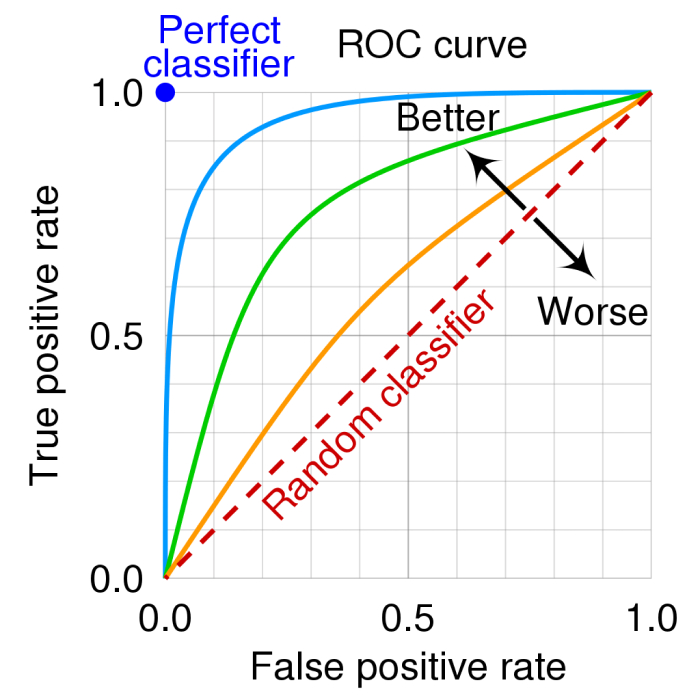
\includegraphics[width=0.5\textwidth]{src/roc-curveUp.jpg}
    \caption{Visualization of the ROC curve. The x-axis represents the false positive rate (FPR), while the y-axis represents the true positive rate (TPR). The diagonal line represents a random classifier, whil the linies above it represent classifiers with varying levels of performance\cite{ROCEG}.}
    \label{fig:roc_curve}
\end{figure}

The Receiver Operating Characteristic (ROC) curve illustrates the diagnostic ability of a classifier as its decision threshold is varied\cite{GoogleDevelopersROCAUC}. For each threshold—i.e., the probability above which a sample is classified into a given class—the true positive rate (TPR) and false positive rate (FPR) are computed:

\[
\text{TPR} = \frac{\text{TP}}{\text{TP} + \text{FN}}, \quad
\text{FPR} = \frac{\text{FP}}{\text{FP} + \text{TN}}
\]

Each \((\text{FPR}, \text{TPR})\) pair is plotted as a point in 2D space, with FPR on the x-axis and TPR on the y-axis. The collection of these points forms the ROC curve. A perfect classifier corresponds to the point (0, 1), indicating no false positives and all true positives, while a random classifier produces a curve along the diagonal from (0, 0) to (1, 1). Example of such curves is shown in figure~\ref{fig:roc_curve}.


\subsubsection{Area Under the Curve (AUC)}

\begin{figure}[H]
    \centering
    \begin{minipage}[t]{0.45\textwidth}
        \centering
        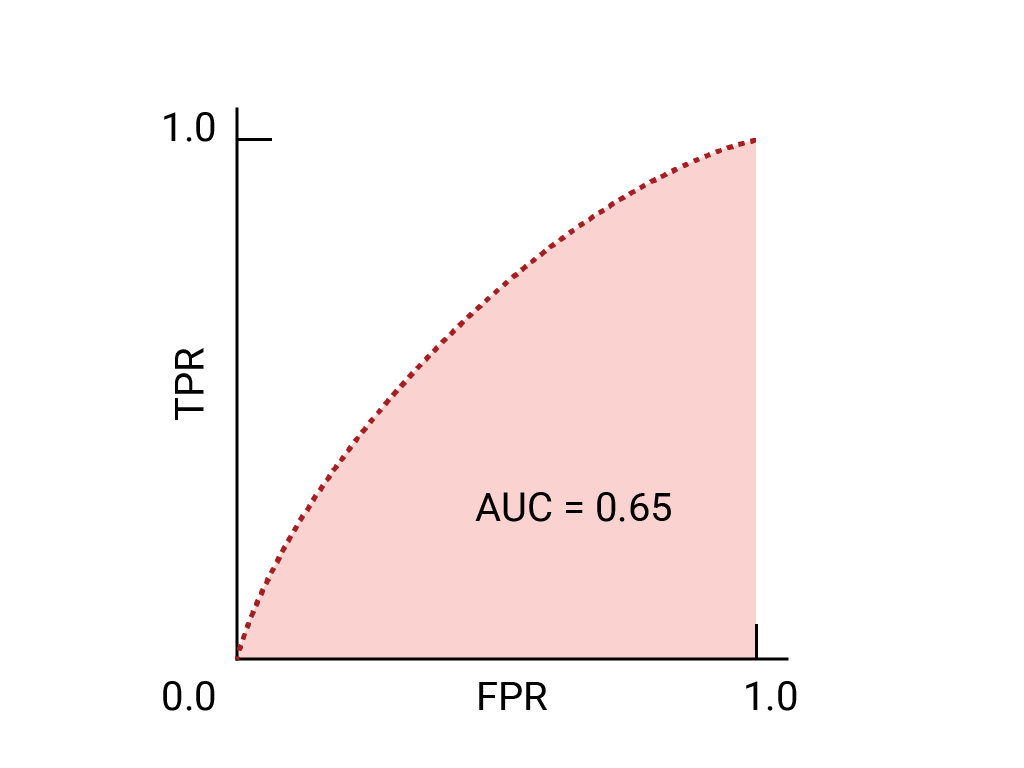
\includegraphics[width=\textwidth]{src/auc_0-65.png}
        % \caption{Caption for conv1.pdf}
    \end{minipage}
    % \hfill
    \begin{minipage}[t]{0.45\textwidth}
        \centering
        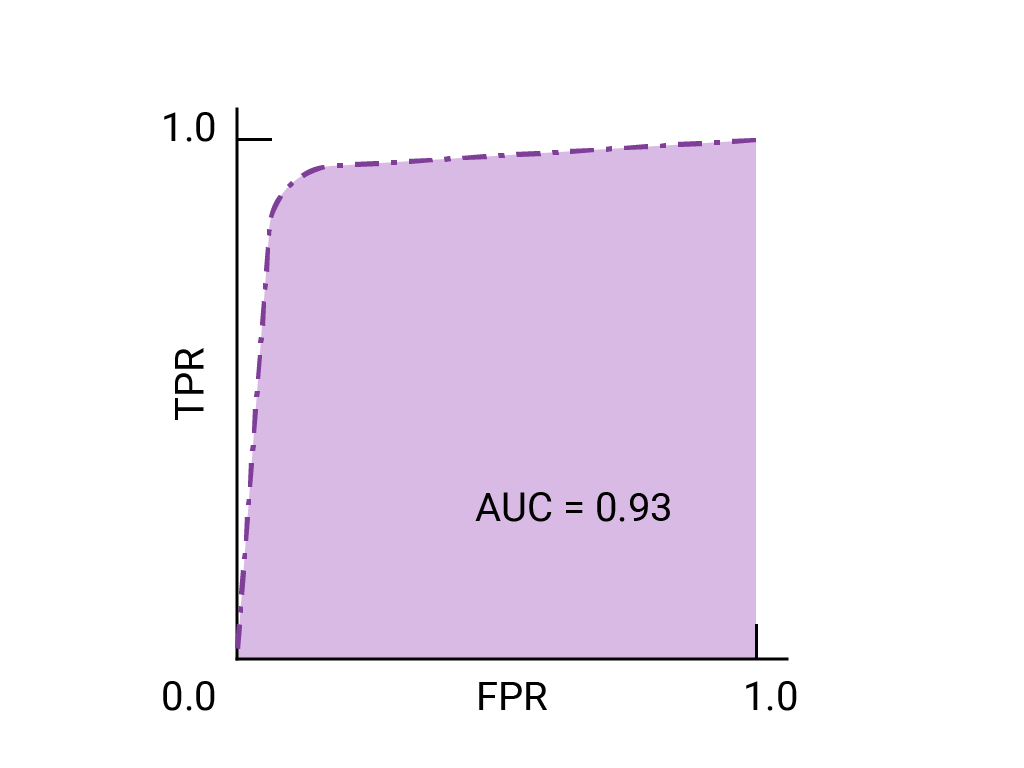
\includegraphics[width=\textwidth]{src/auc_0-93.png}
        % \caption{Caption for conv2.pdf}
    \end{minipage}
    \caption{ROC and AUC of two hypothetical models. The curve on the right, with a greater AUC, represents the better of the two models\cite{GoogleDevelopersROCAUC}.}
\end{figure}


The Area Under the Curve (AUC) summarizes the ROC curve in a single scalar value between 0 and 1. An AUC of 0.5 indicates random guessing, while an AUC of 1.0 represents perfect classification. AUC can be interpreted as the probability that the model, if given a randomly chosen positive and negative example, will rank the positive higher than the negative. The model with greater area under the curve is generally the better one.

\chapter{Convolutional Neural Networks (CNNs)}

% \textit{Source:} \url{file:///C:/Users/wojte/Downloads/s13244-018-0639-9.pdf}

All of the information in this section was taken from \cite{CNNExplained}.

Convolutional neural networks (CNNs) are a class of machine learning algorithms designed to automatically and adaptively learn spatial hierarchies of features, ranging from low-level edges to high-level semantic patterns. They consist of stacked convolutional and pooling layers responsible for feature extraction, followed by fully connected layers that perform the final classification. Each layer passes its output to the next, enabling progressively more abstract and complex features to be learned as information flows through the network.

\section{Convolutional Layer}

\begin{figure}[H]
    \centering
    \begin{minipage}[t]{0.48\textwidth}
        \centering
        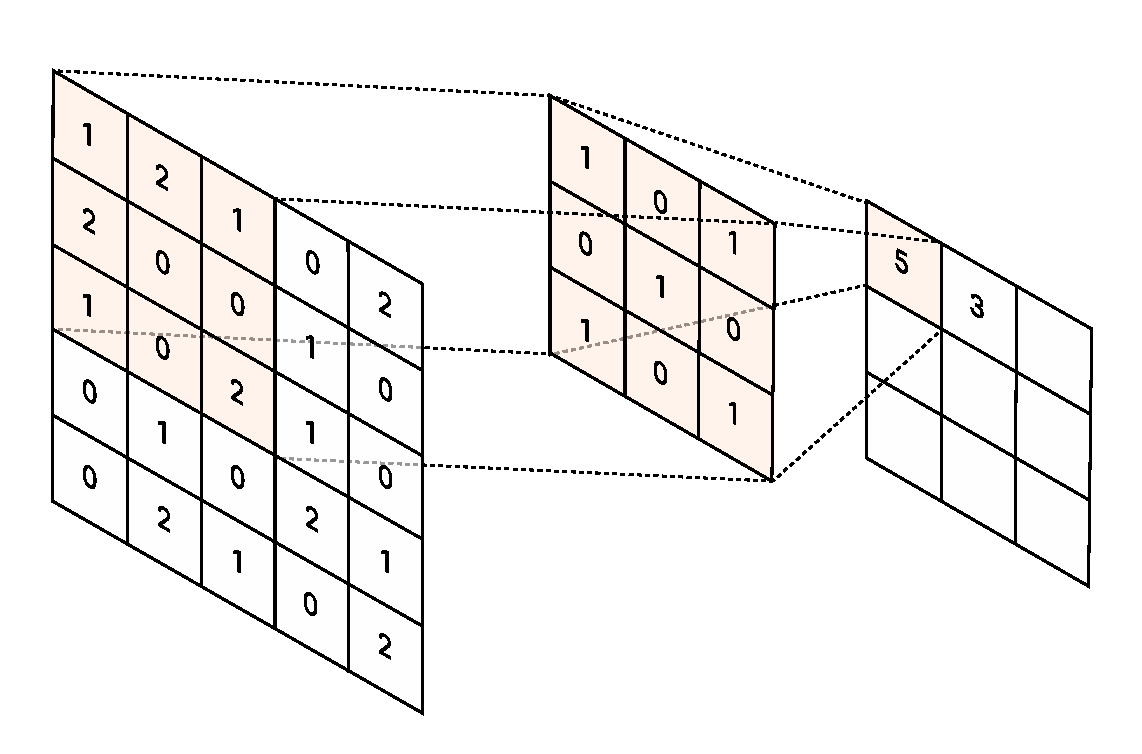
\includegraphics[width=\textwidth]{src/conv1.pdf}
    \end{minipage}
    \hfill
    \begin{minipage}[t]{0.48\textwidth}
        \centering
        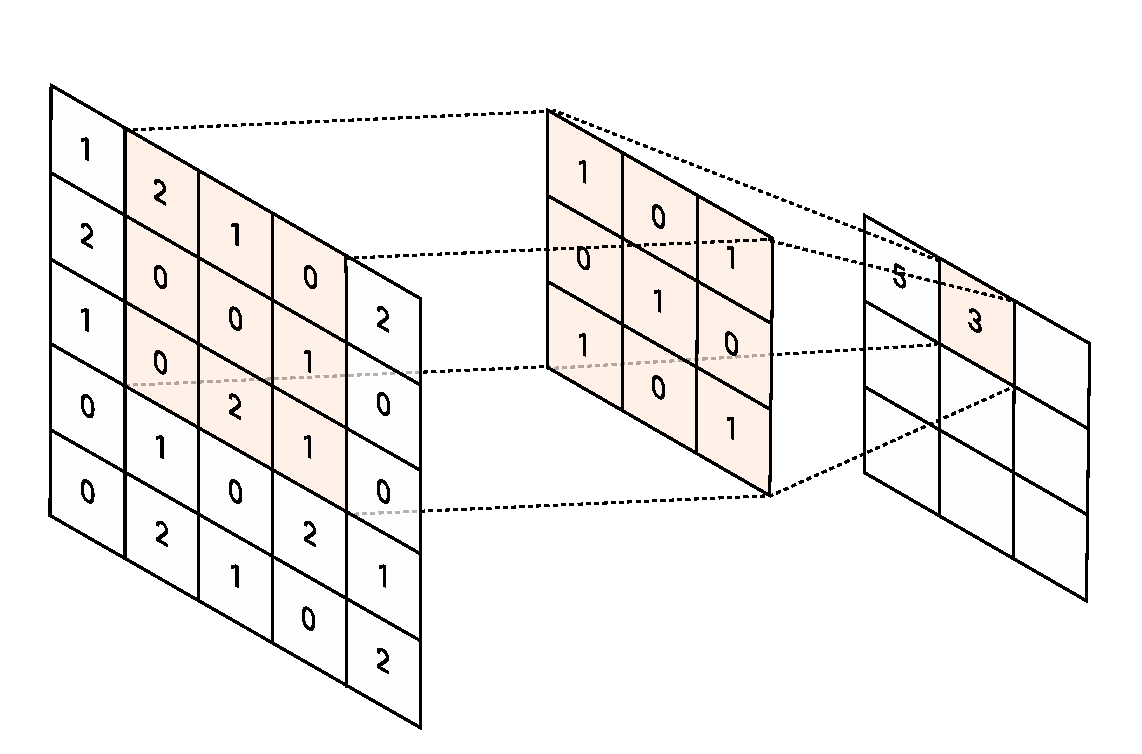
\includegraphics[width=\textwidth]{src/conv2.pdf}
    \end{minipage}
    \caption{Example of convolutional layer operation \cite{Yamashita2018}}
    \label{fig:conv_layer}
\end{figure}

\subsubsection{General Mechanism}

A convolution is a linear operation that involves element-wise multiplication between an input array and a corresponding kernel (also referred to as a \textit{filter}), followed by summation of the resulting products. The kernel is an array of values, typically smaller than the input array, that defines the operation and characterizes the specific features being extracted.

In a convolutional layer, multiple such kernels are applied to every valid subsection of the input array with dimensions matching the kernel (as shown in figure \ref{fig:conv_layer}). The result of each convolution is a single scalar value, which becomes an element of the output feature map. To preserve or control the spatial dimensions of the output, \textit{padding} may be applied to the input array, typically by adding zeros around its border.

The output of a convolutional layer is an array (or tensor) with reduced spatial dimensions (depending on the padding and stride) and a number of channels equal to the number of kernels employed in the layer.

\subsubsection{Feature Recognition Mechanism}

During backpropagation, each element of every kernel is treated as a learnable parameter and is optimized using gradient descent. The gradients of these parameters are computed with respect to each input element (more precisely, with respect to each considered subsection of the input array). These gradients are then aggregated—typically by averaging—and the kernel parameters are updated accordingly.

The general objective is for the kernels to adjust themselves to specific features of the input image—that is, to produce high activation values when a particular feature is present and low values when it is absent. The calculated gradients for each subsection of the input array depend on the values of the inputs. Consequently, it is assumed that during training, the elements of the kernels are updated in such a way that each kernel learns to recognize a distinct feature in the input array.

\begin{figure}[H]
    \centering
    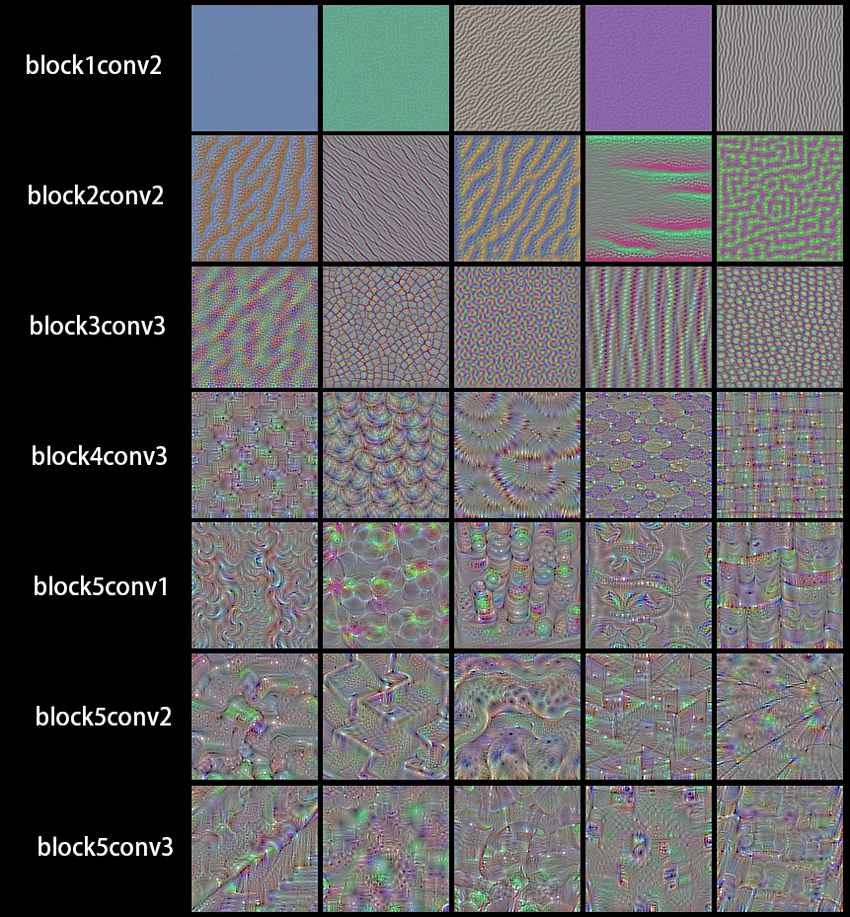
\includegraphics[width=0.55\textwidth]{src/convViz.png}
    \caption{Visualization of feature maps learned by different convolutional layers of a CNN. Each row corresponds to a different convolutional layer (from early to late), and each column shows a visualization of the input pattern that maximally activates a specific filter. \cite{exCNN}}
    \label{fig:convviz}
\end{figure}

Figure~\ref{fig:convviz} shows visualizations of features that maximally activate a selection filters across different convolutional layers of a CNN taken from \cite{activations}.

In the early layers (e.g., \texttt{block1conv2}, \texttt{block2conv2}), the filters detect simple low-level features such as edges, colors, and textures. In deeper layers (e.g., \texttt{block4conv3}, \texttt{block5conv3}), the patterns become increasingly complex, capturing higher-level concepts.

\section{Pooling Layer}

\begin{figure}[H]
    \centering
    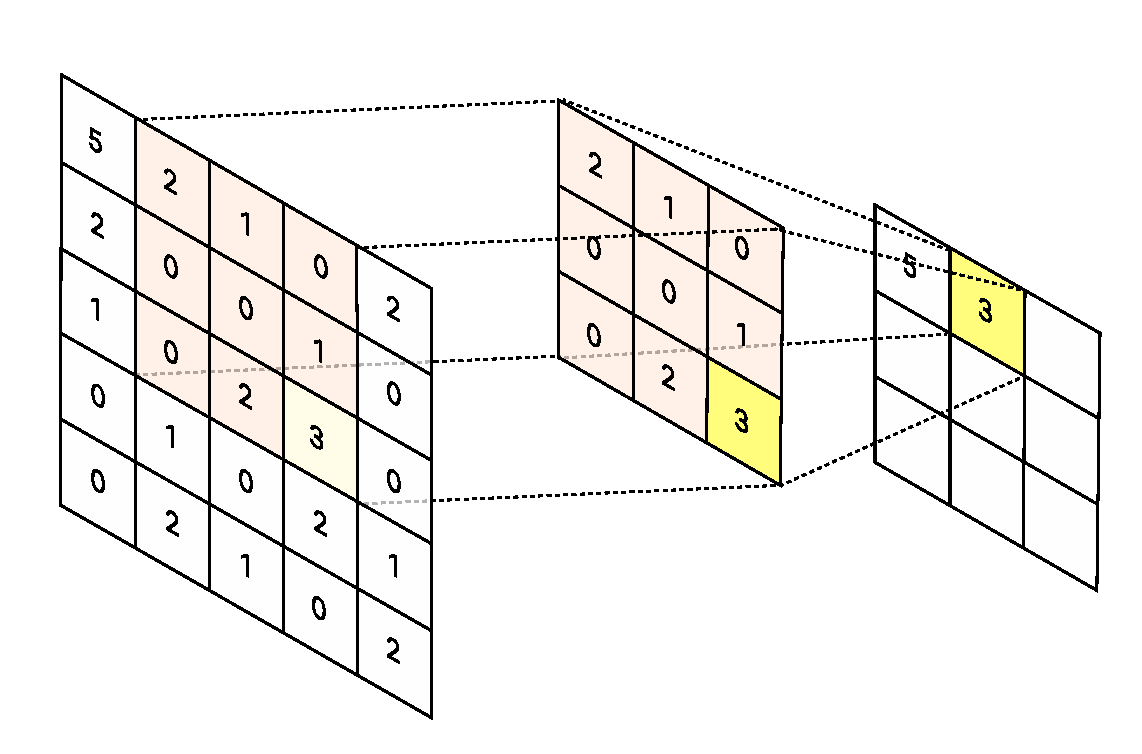
\includegraphics[width=0.8\textwidth]{src/pool1.pdf}
    \caption{Example of max pooling layer operation \cite{Yamashita2018}}
\end{figure}

A pooling layer is a downsampling operation used to reduce the spatial dimensions of feature maps while preserving salient information. The specific pooling method used in each layer is selected based on its effectiveness for the given classification task, typically determined through empirical evaluation. Among the available techniques, \textit{max pooling}—which selects the maximum value within a specified region—is the most commonly employed approach.

Pooling layers operate independently on each feature map (channel), where a channel corresponds to a set of activations produced by a single convolutional filter, and do not involve learnable parameters. By summarizing local regions, they can ensure invariance to small translations and reduce computational complexity in subsequent layers. Similar to convolutional layers, padding and stride can be used to control the spatial dimensions of the output.

\section{Multi-Layer Perceptron}

\begin{figure}[H]
\centering
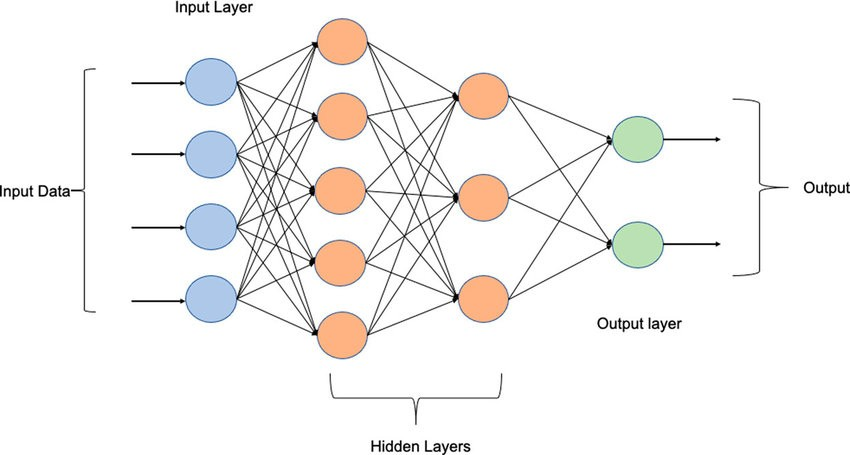
\includegraphics[width=0.8\textwidth]{src/mlp.jpg}
\caption{Illustration of a multi-layer perceptron architecture\cite{mplGraphEG}}
\end{figure}

A multi-layer perceptron (MLP) is a neural network composed of multiple fully connected layers (ie. a layer where each neuron receives input from every neuron in the previous layer). The MLP used in this context typically consists of several layers with progressively smaller numbers of neurons, culminating in an output layer tailored to the classification task.

In classical CNN architectures, the output of the final convolution or pooling layer is flattened and passed into a multi-layer perceptron to perform the final classification.

\section{Complete CNN}

\begin{figure}[H]
    \centering
    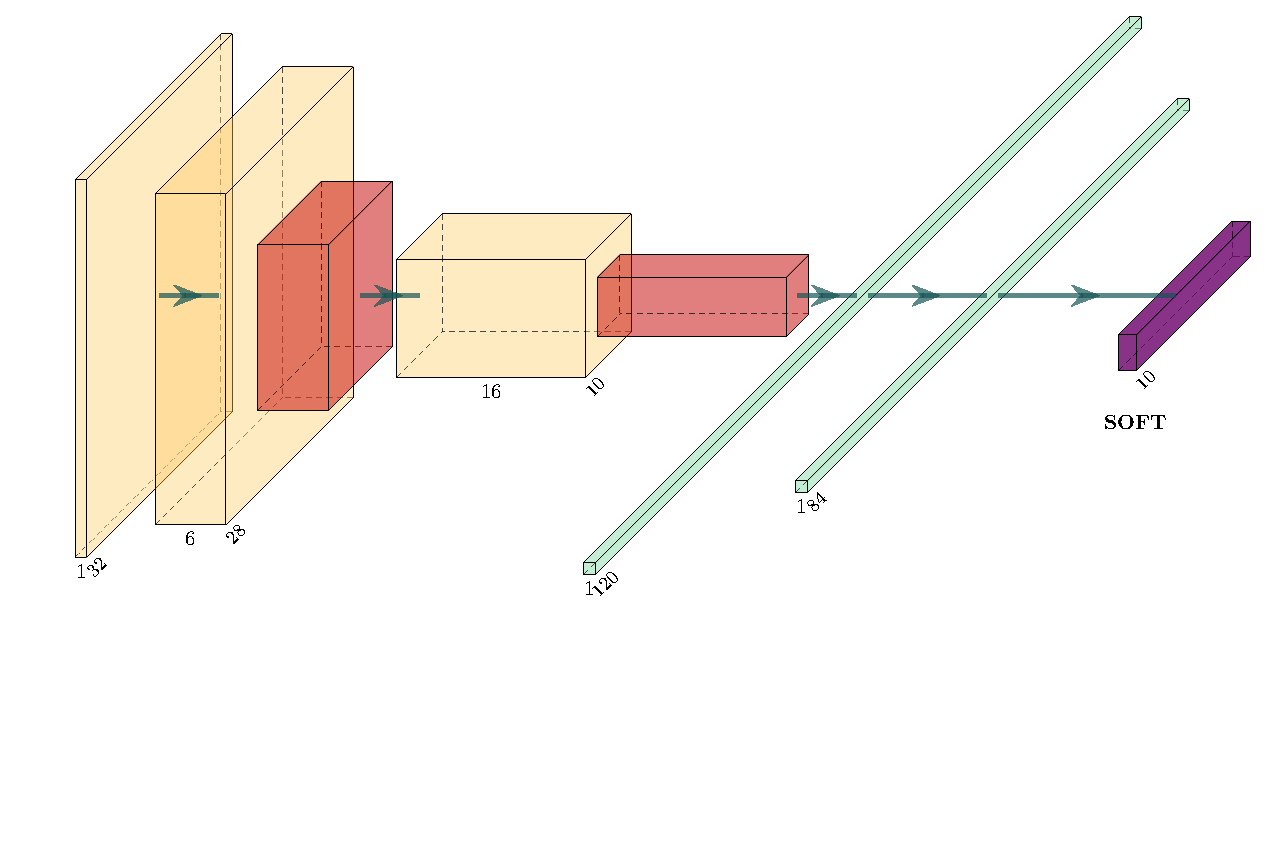
\includegraphics[width=0.7\textwidth]{src/lenet.pdf}
    \caption{Schematic architecture of a simple convolutional neural network (CNN). Each 3D block represents a data tensor at a given stage of the network. The width and height of the blocks reflect the spatial resolution of feature maps, while the depth indicates the number of channels (e.g., filters in convolutional layers or neurons in fully connected layers). The color changes distinguish between different types of operations: convolution (yellow), activation/pooling (red), flattening (transition to vector), and fully connected layers (blue). Purple represents a softmax layer. The numbers next to the blocks denote either the number of output channels or neurons or the spatial dimensions\cite{Iqbal2018PlotNeuralNet}.}
    \label{fig:cnn_architecture}
\end{figure}

The first layers of the neural network consist of a hierarchy of convolution and pooling layers, each taking the output of the previous layer as input. The output of the final convolutional or pooling layer is then passed to a fully connected layer, which performs the final classification.

During training, the network first attempts to classify a batch of input elements. The predicted output is then compared to the true class labels, and a loss value is computed. This loss is subsequently backpropagated through the network, and the gradients for all learnable parameters are calculated. Finally, a step of gradient descent is performed, and the learnable parameters are updated accordingly.

\section{Networks used}

Two different architectures were used to classify the images, specifics of which are described below. Both networks were trained on the same dataset, with the same hyperparameters, to ensure a fair comparison of their respective performance.

\subsection{LeNet-like network}

\begin{figure}[H]
    \centering
    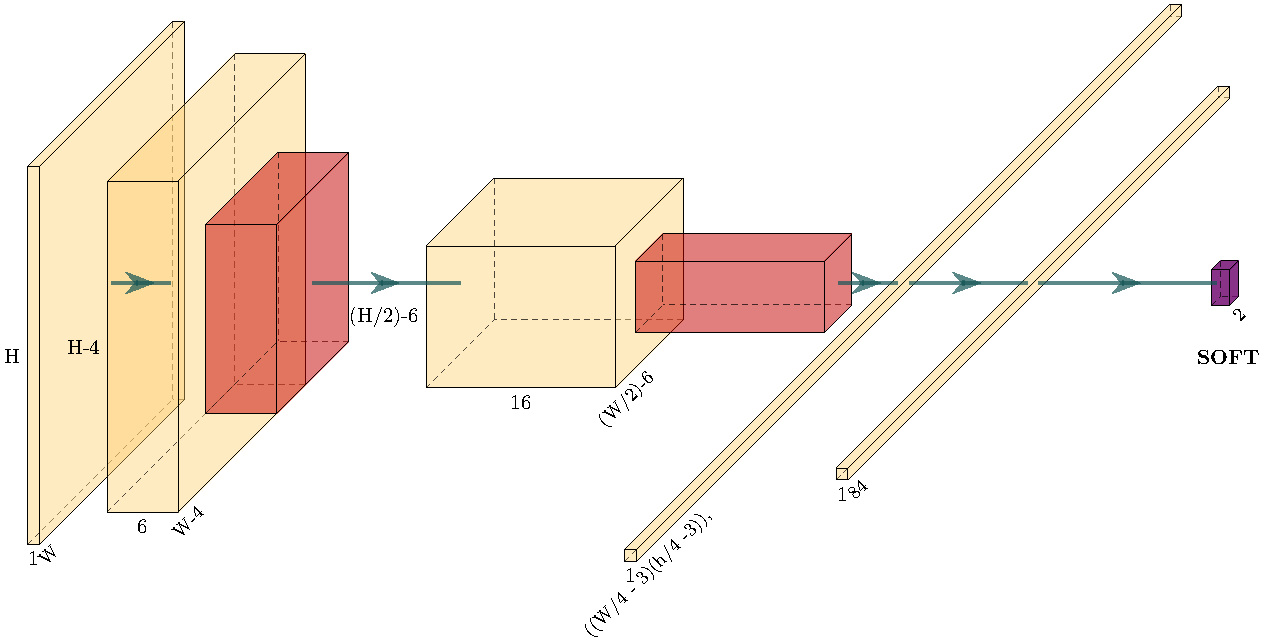
\includegraphics[width=0.8\textwidth]{src/LeNetLike.pdf}
    \caption{Graphical representation of the LeNet-inspired CNN used \cite{Iqbal2018PlotNeuralNet}}
    \label{fig:lenetLike_architecture}
\end{figure}

\begin{table}[H]
\centering
\caption{Summary of convolutional and pooling layers in the \texttt{SimpleCNN} architecture.}
\begin{tabular}{|l|c|c|c|c|}
\hline
\textbf{Layer Type} & \textbf{Output Channels} & \textbf{Kernel Size} & \textbf{Stride} & \textbf{Output Size} \\
\hline
Conv2d (conv1)       & 6   & 5×5 & 1 & 28×28 \\
AvgPool2d (pool1)    & -   & 2×2 & 2 & 14×14 \\
Conv2d (conv2)       & 16  & 5×5 & 1 & 10×10 \\
AvgPool2d (pool2)    & -   & 2×2 & 2 & 5×5 \\
Conv2d (conv3)       & 120 & 5×5 & 1 & 1×1 \\
\hline
\end{tabular}
\label{tab:simplecnn_layers}
\end{table}


One of the architectures used was based on the classical LeNet-5 convolutional neural network, originally developed for digit recognition. It is a shallow network originally designed for small-scale image classification tasks\cite{LeNet}.

This architecture is summarized in Table~\ref{tab:simplecnn_layers} and visualized in figure~\ref{fig:lenetLike_architecture}.

\subsection{AlexNet-like CNN}

\begin{figure}[H]
    \centering
    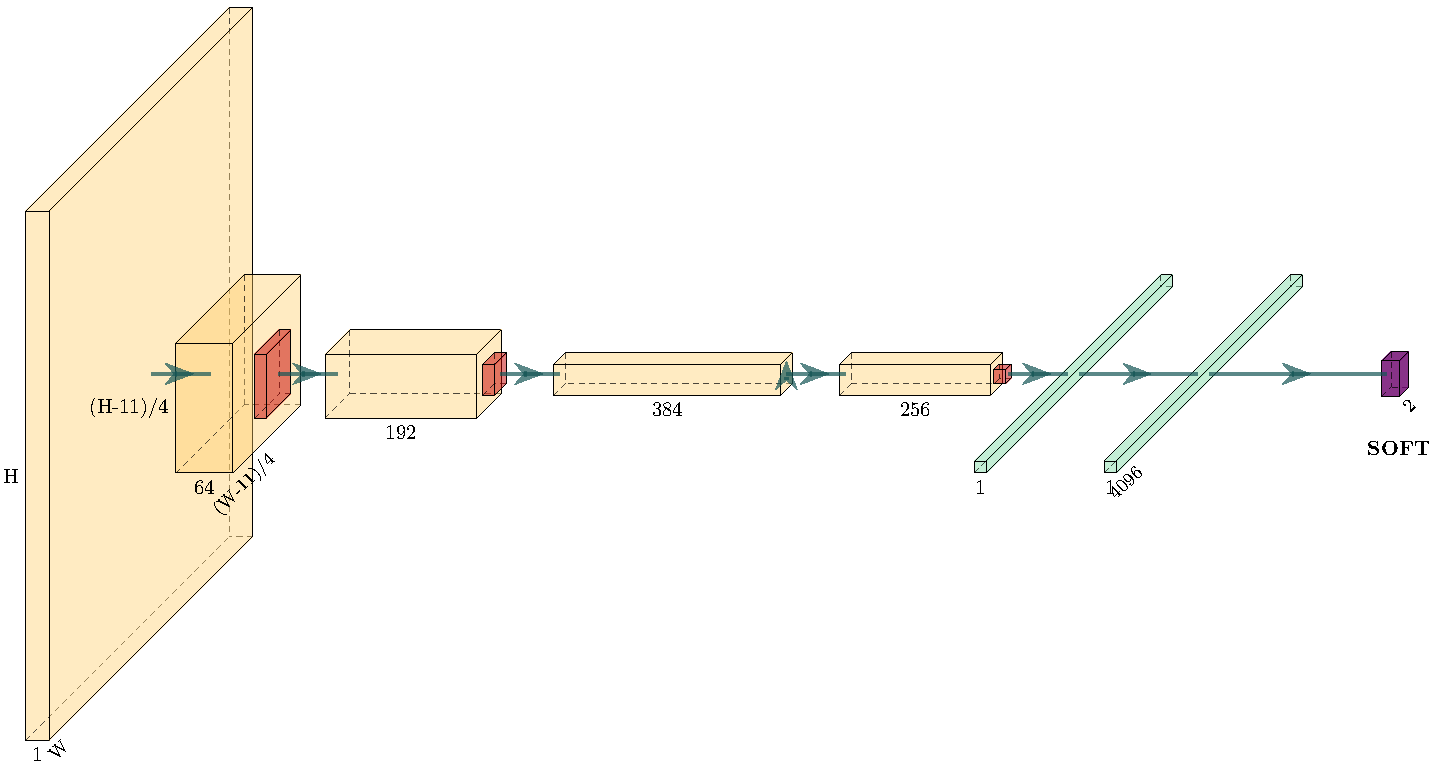
\includegraphics[width=0.8\textwidth]{src/AlexNetLike.pdf}
    \caption{Example layout of a simple CNN\cite{Iqbal2018PlotNeuralNet}}
    \label{fig:alexnetLike_architecture}
\end{figure}

\begin{table}[H]
\centering
\caption{Summary of convolutional and pooling layers in the \texttt{AlexCNNLayer} architecture.}
\begin{tabular}{|l|c|c|c|c|}
\hline
\textbf{Layer Type} & \textbf{Output Channels} & \textbf{Kernel Size} & \textbf{Stride} & \textbf{Padding} \\
\hline
Conv2d (conv1) & 64 & 11×11 & 4 & 2 \\
MaxPool2d (pool1) & - & 3×3 & 2 & 0 \\
Conv2d (conv2) & 192 & 5×5 & 1 & 2 \\
MaxPool2d (pool2) & - & 3×3 & 2 & 0 \\
Conv2d (conv3) & 384 & 3×3 & 1 & 1 \\
Conv2d (conv4) & 256 & 3×3 & 1 & 1 \\
Conv2d (conv5) & 256 & 3×3 & 1 & 1 \\
MaxPool2d (pool3) & - & 3×3 & 2 & 0 \\
\hline
\end{tabular}
\label{tab:alexcnn_layers}
\end{table}


Another architecture utilized was a modified version of the AlexNet model, originally developed for the ImageNet Large Scale Visual Recognition Challenge (ILSVRC). The general hope being that the fact that it's significantly deeper and wider than LeNet would enable classify the images more effectively\cite{AlexNETpub}.

This architecture is summarized in Table~\ref{tab:alexnet_architecture} and visualized in figure~\ref{fig:alexnetLike_architecture}.

\subsection{Training Procedure}

Both networks were trained using a training routine implemented in PyTorch. The training process operated on a combined dataset and dynamically inferred input dimensions from a sample image. Image preprocessing included optional downscaling using nearest-neighbor interpolation, followed by conversion to tensor format. The models were optimized using stochastic gradient descent (SGD) with a fixed learning rate of 0.0005 and a momentum of 0.9. Cross-entropy loss was used as the objective function. Training was conducted for 10 epochs with a batch size of 16. During each epoch, loss and classification accuracy were recorded.

The dataset was split into training, validation, and test sets in a 70/15/15 ratio. Networks were trained on the training set, and their performance was evaluated on the validation set. The best-performing model on the validation set was selected for final evaluation on the test set, which consisted of data the model had no access to previously. Training was conducted separately on the full dataset and on a subset limited to the top 50\% of most energetic lepton interactions. For simplicity, only data from plane2 was used. Input images were scaled down to 0.33 and 0.5 of their original size. Confusion matrices were computed for all trained models, and results were compared. F1 scores and ROC curves were calculated for the best-performing models. Results of the training are described in the next chapter.

\section{Results}

\subsection{LeNet}

\begin{figure}[H]
    \centering
    \begin{subfigure}{\textwidth}
        \centering
        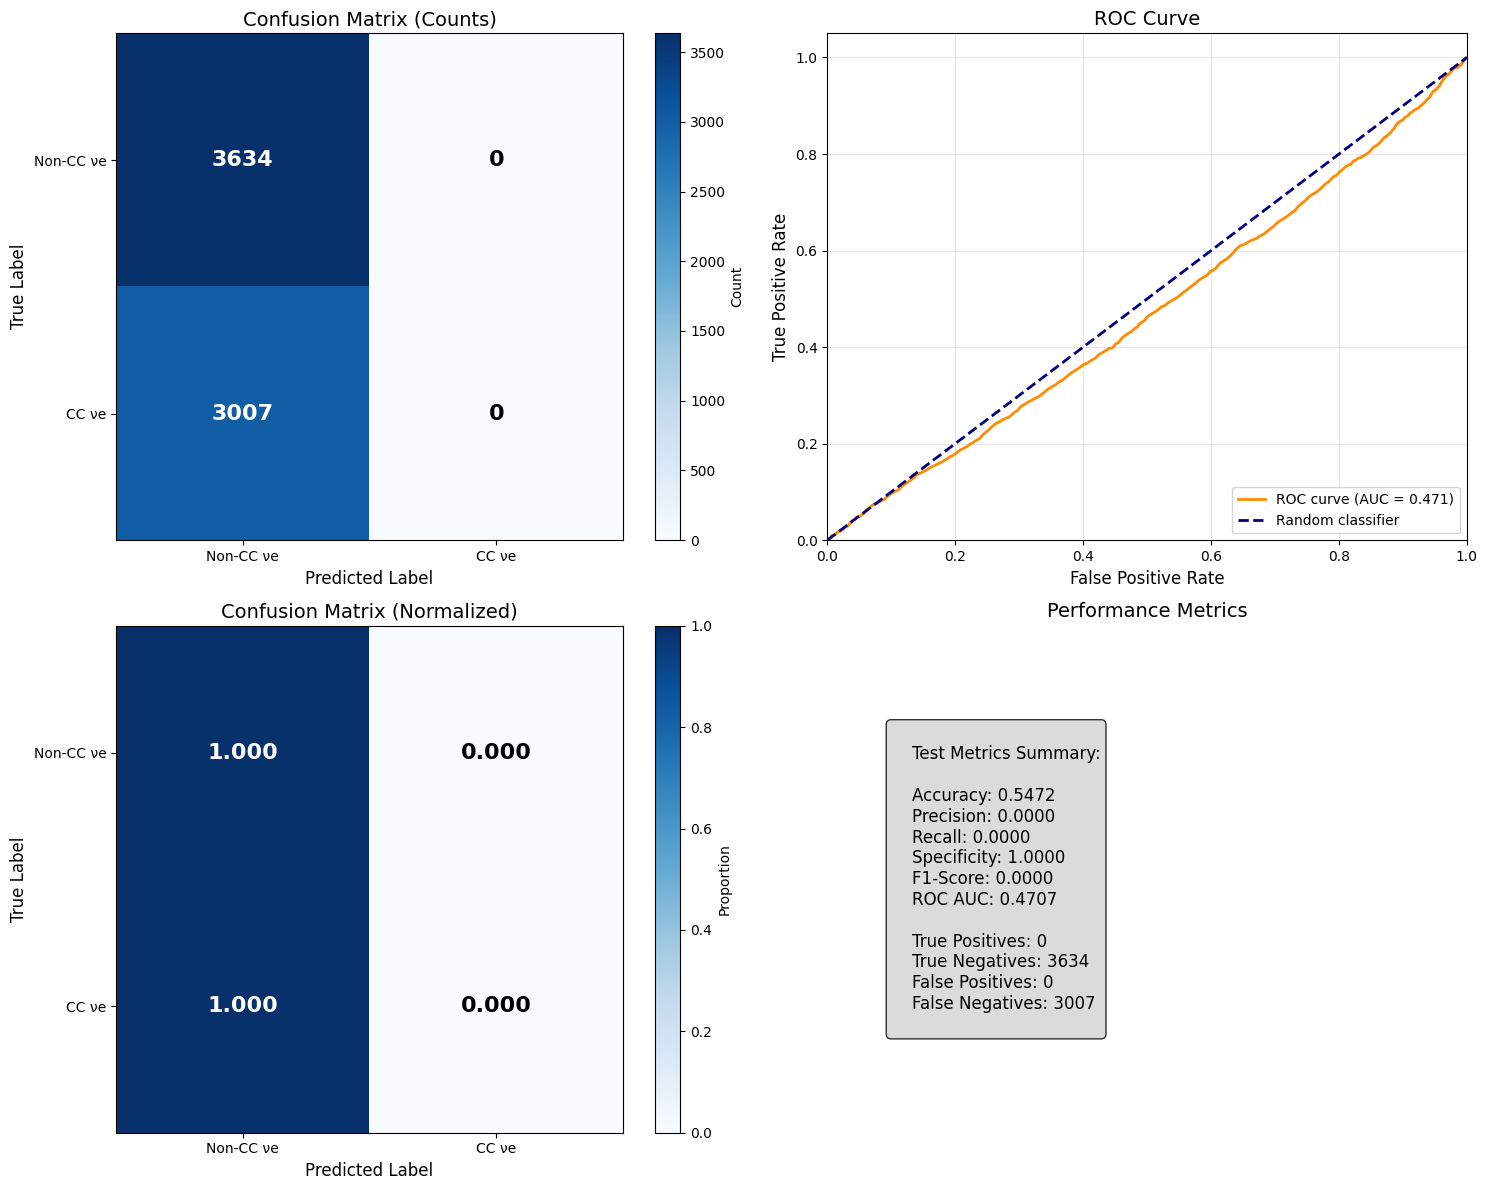
\includegraphics[width=0.9\textwidth]{src/LeNET_1ch_full_dataset_scale033.png}
        % \caption{Caption for the first image}
        \label{fig:Lefull33sub1}
    \end{subfigure}
    
    \vspace{1cm}
    
    \begin{subfigure}{\textwidth}
        \centering
        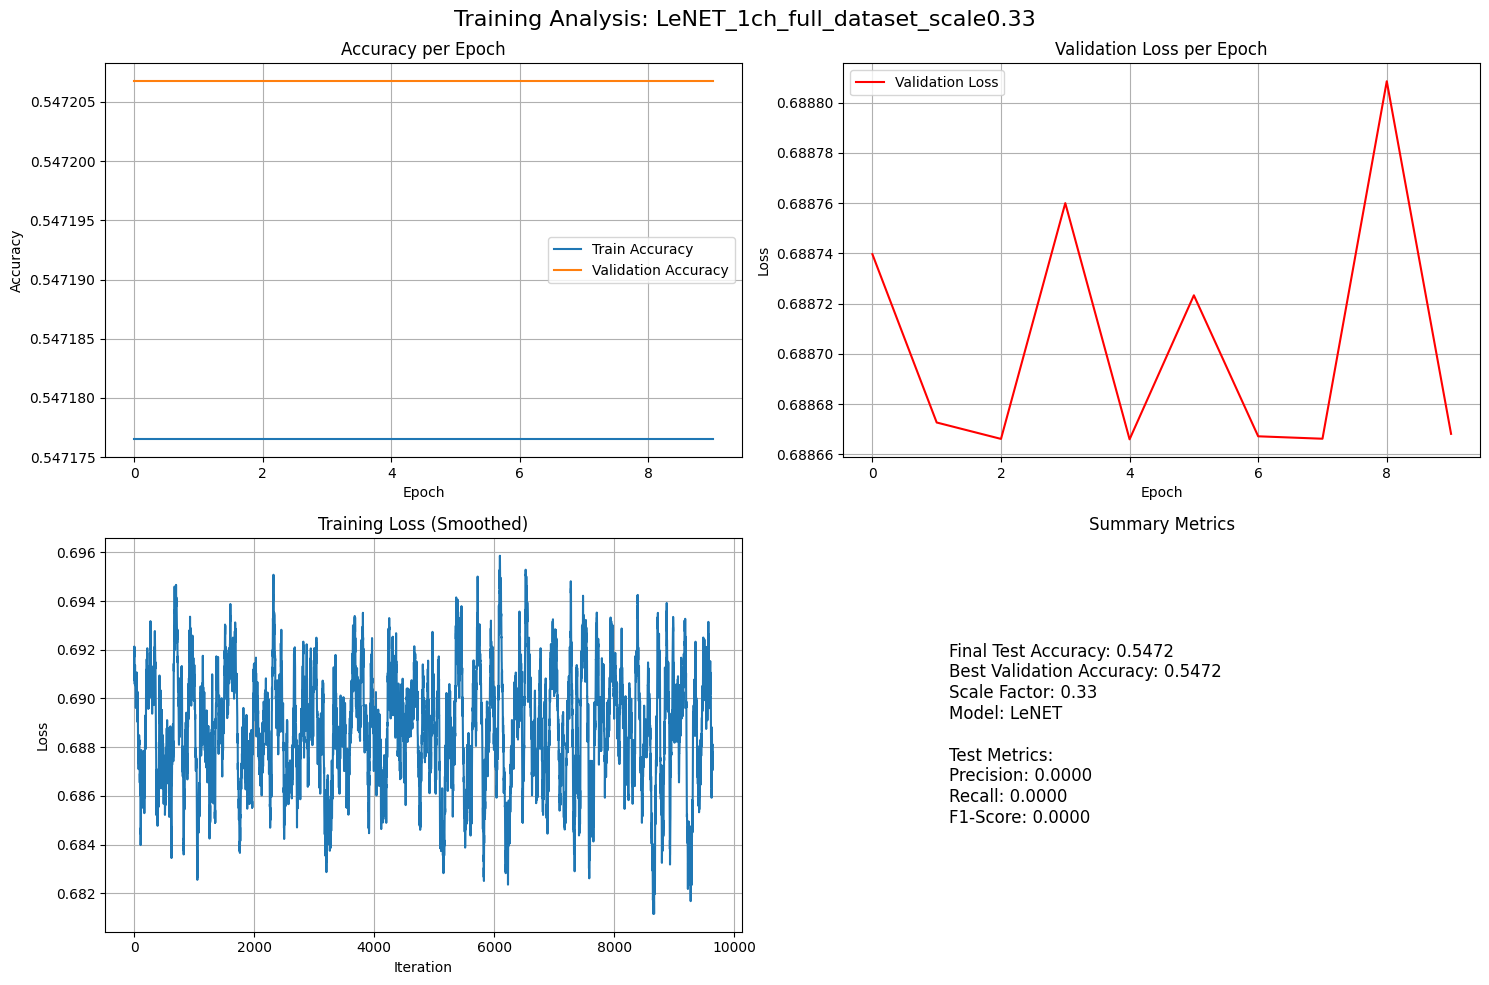
\includegraphics[width=0.9\textwidth]{src/LeNET_1ch_full_dataset_scale033loss.png}
        % \caption{Caption for the second image}
        \label{fig:Lefull33sub2}
    \end{subfigure}
    \caption{LeNET training results on the full dataset with images scaled down to 0.33 of their original size.}
    \label{fig:Lefull33stacked}
\end{figure}

\newpage

% \begin{figure}[H]
%     \centering
%     \begin{subfigure}{\textwidth}
%         \centering
%         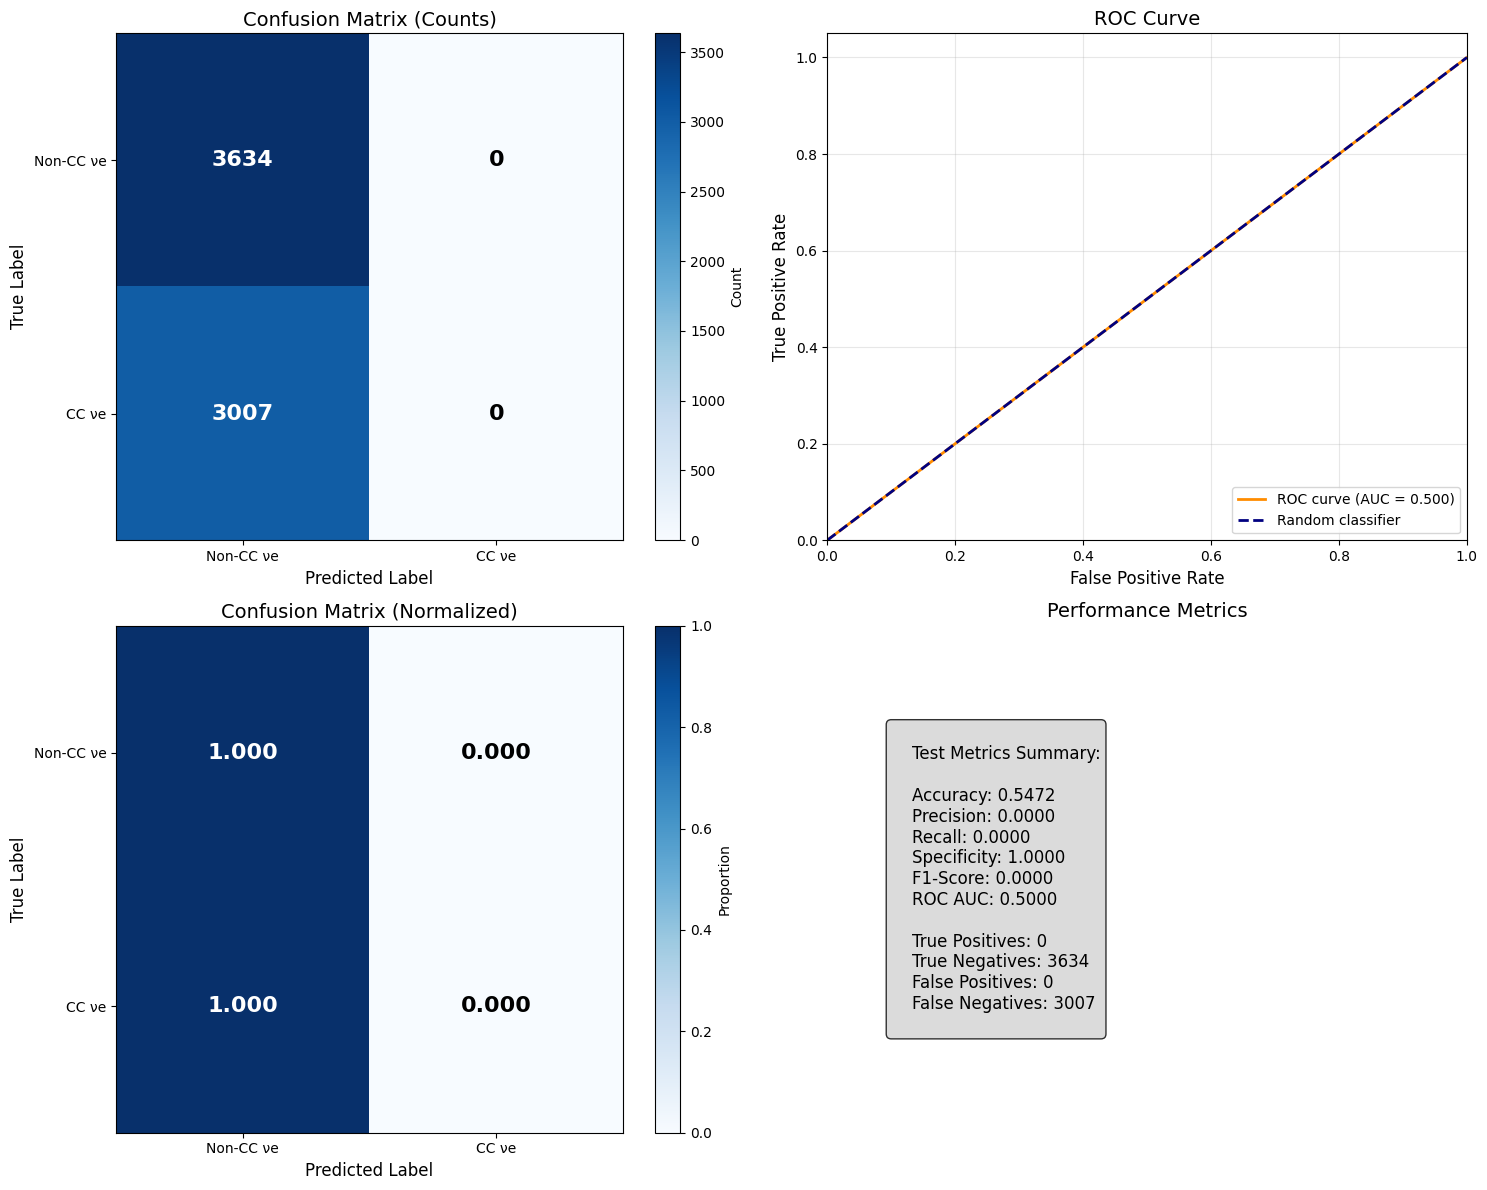
\includegraphics[width=0.9\textwidth]{src/LeNET_1ch_full_dataset_scale05.png}
%         % \caption{Caption for the first image}
%         \label{fig:Lefull5sub1}
%     \end{subfigure}
    
%     \vspace{1cm}
    
%     \begin{subfigure}{\textwidth}
%         \centering
%         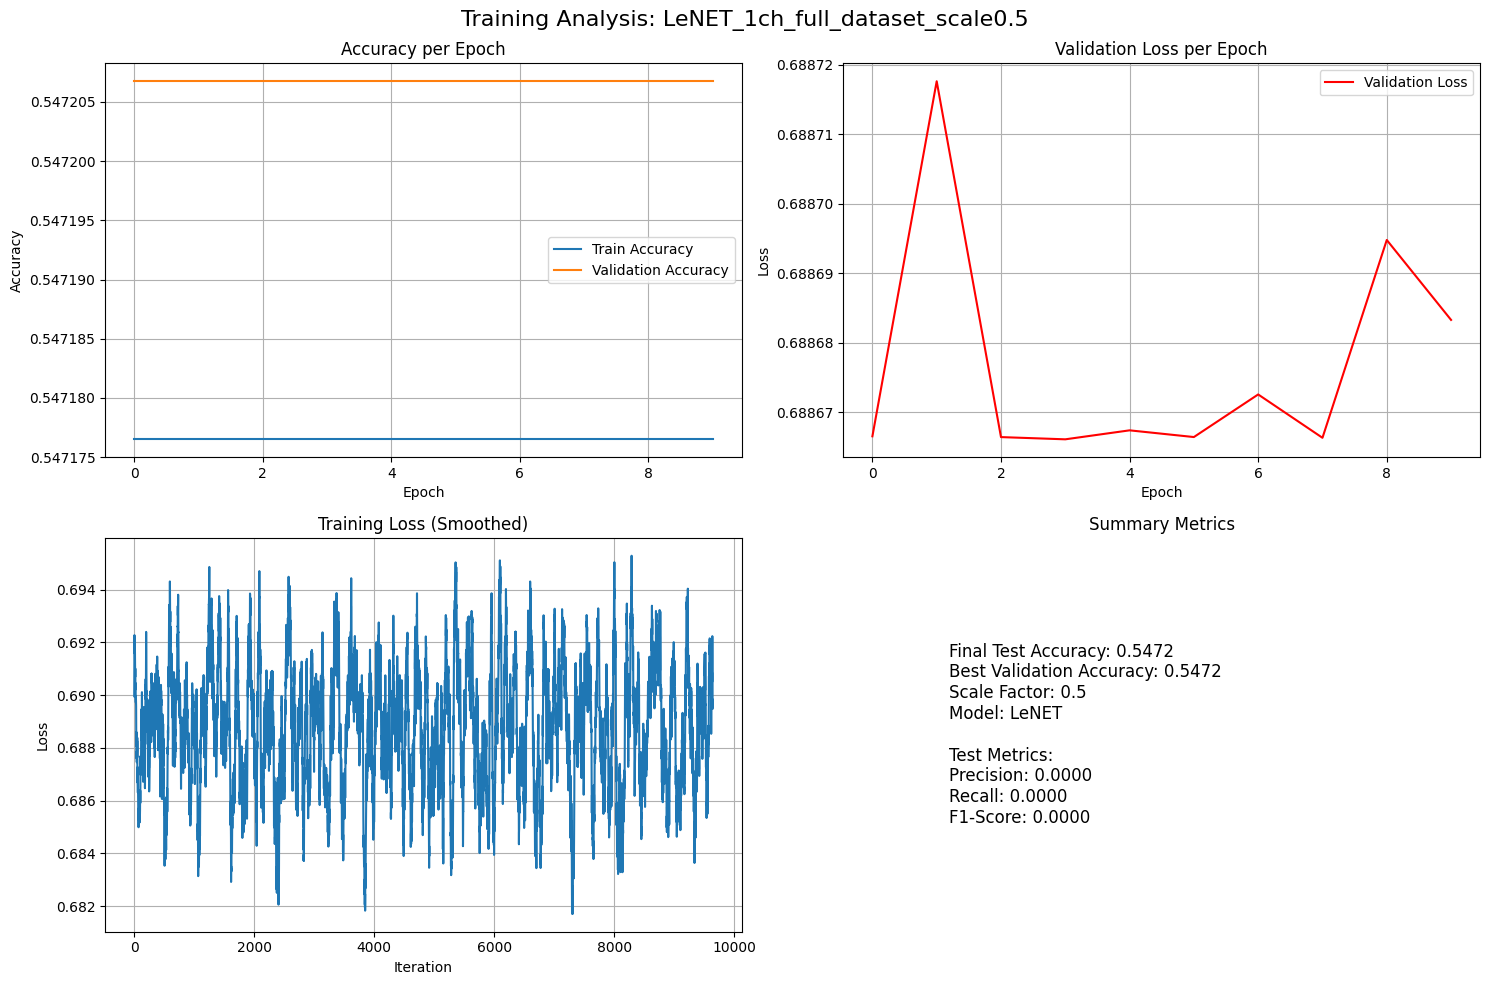
\includegraphics[width=0.9\textwidth]{src/LeNET_1ch_full_dataset_scale05loss.png}
%         % \caption{Caption for the second image}
%         \label{fig:Lefull5sub2}
%     \end{subfigure}
%     \caption{LeNET training results on the full dataset with images scaled down to 0.5 of their original size.}
%     \label{fig:Lefull5stacked}
% \end{figure}

% \newpage

% \begin{figure}[H]
%     \centering
%     \begin{subfigure}{\textwidth}
%         \centering
%         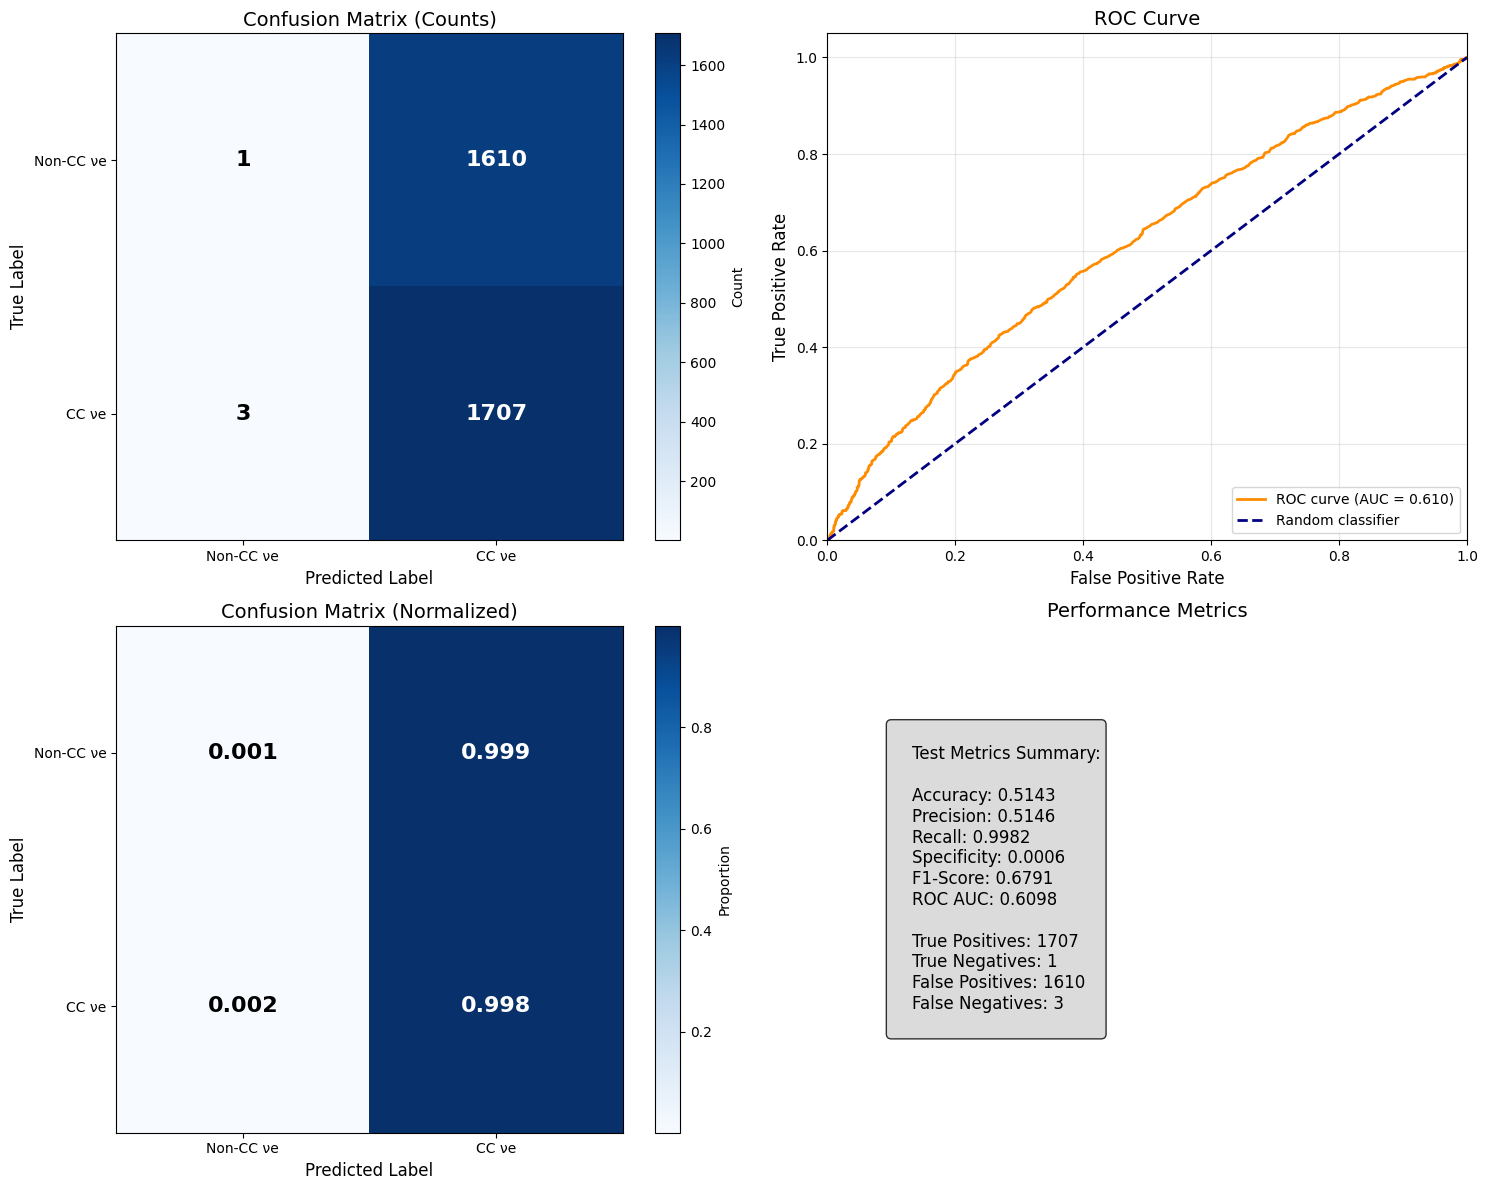
\includegraphics[width=0.9\textwidth]{src/LeNET_1ch_top50_dataset_scale033.png}
%         % \caption{Caption for the first image}
%         \label{fig:Letop5033sub1}
%     \end{subfigure}
    
%     \vspace{1cm}
    
%     \begin{subfigure}{\textwidth}
%         \centering
%         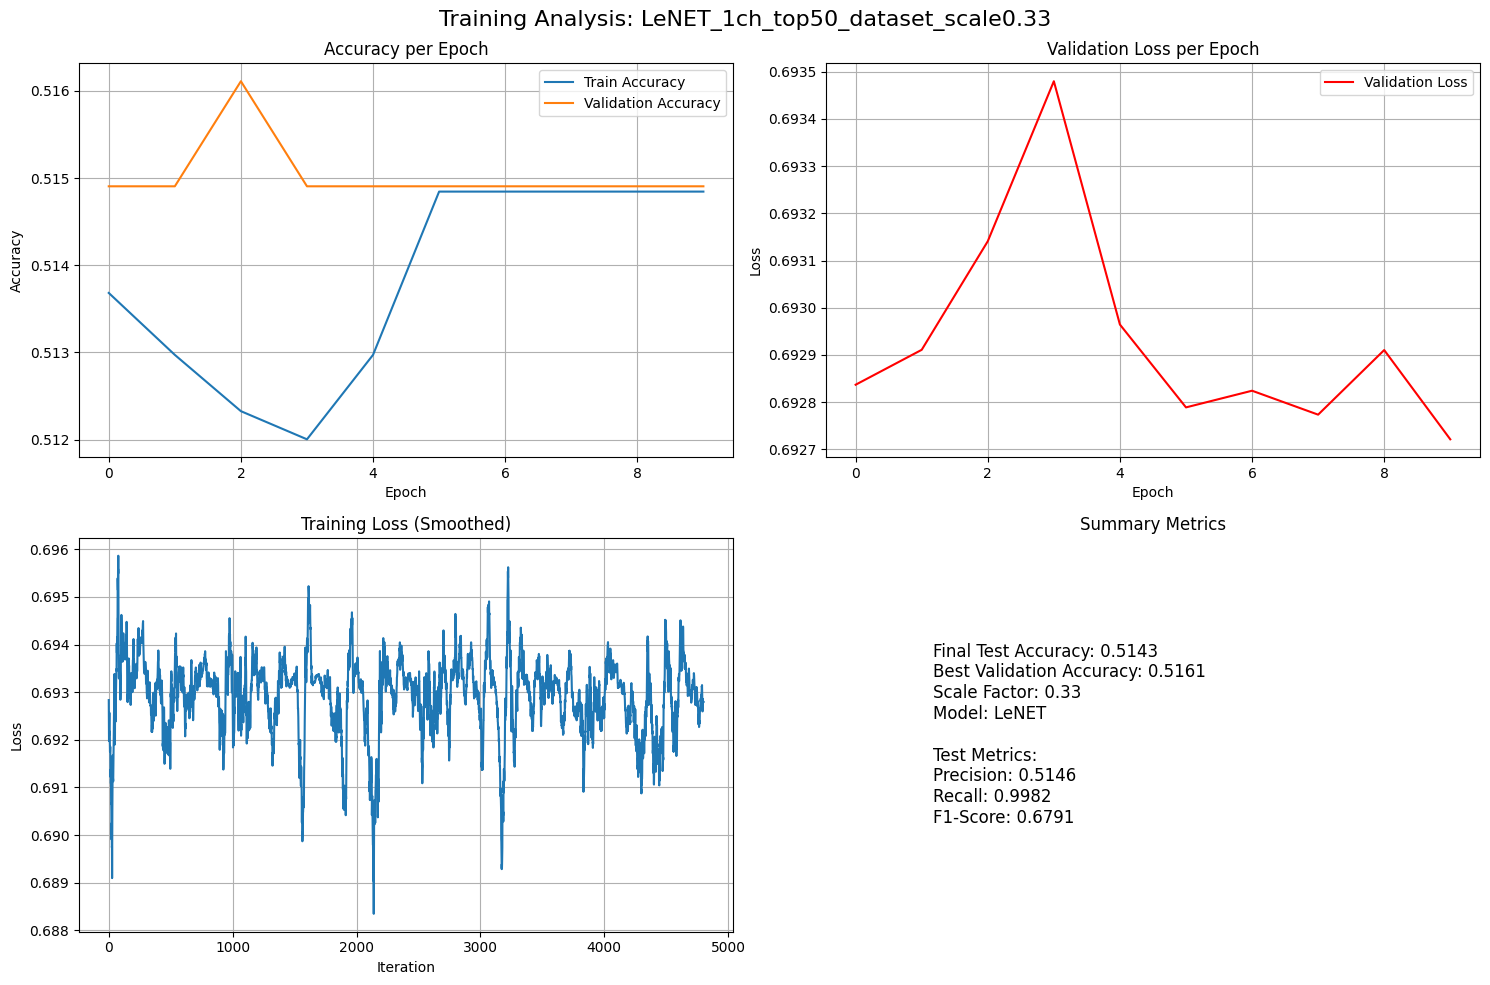
\includegraphics[width=0.9\textwidth]{src/LeNET_1ch_top50_dataset_scale033loss.png}
%         % \caption{Caption for the second image}
%         \label{fig:Letop5033sub2}
%     \end{subfigure}
%     \caption{LeNET training results on the top50 dataset with images scaled down to 0.33 of their original size.}
%     \label{fig:Letop5033stacked}
% \end{figure}

% \newpage

% \begin{figure}[H]
%     \centering
%     \begin{subfigure}{\textwidth}
%         \centering
%         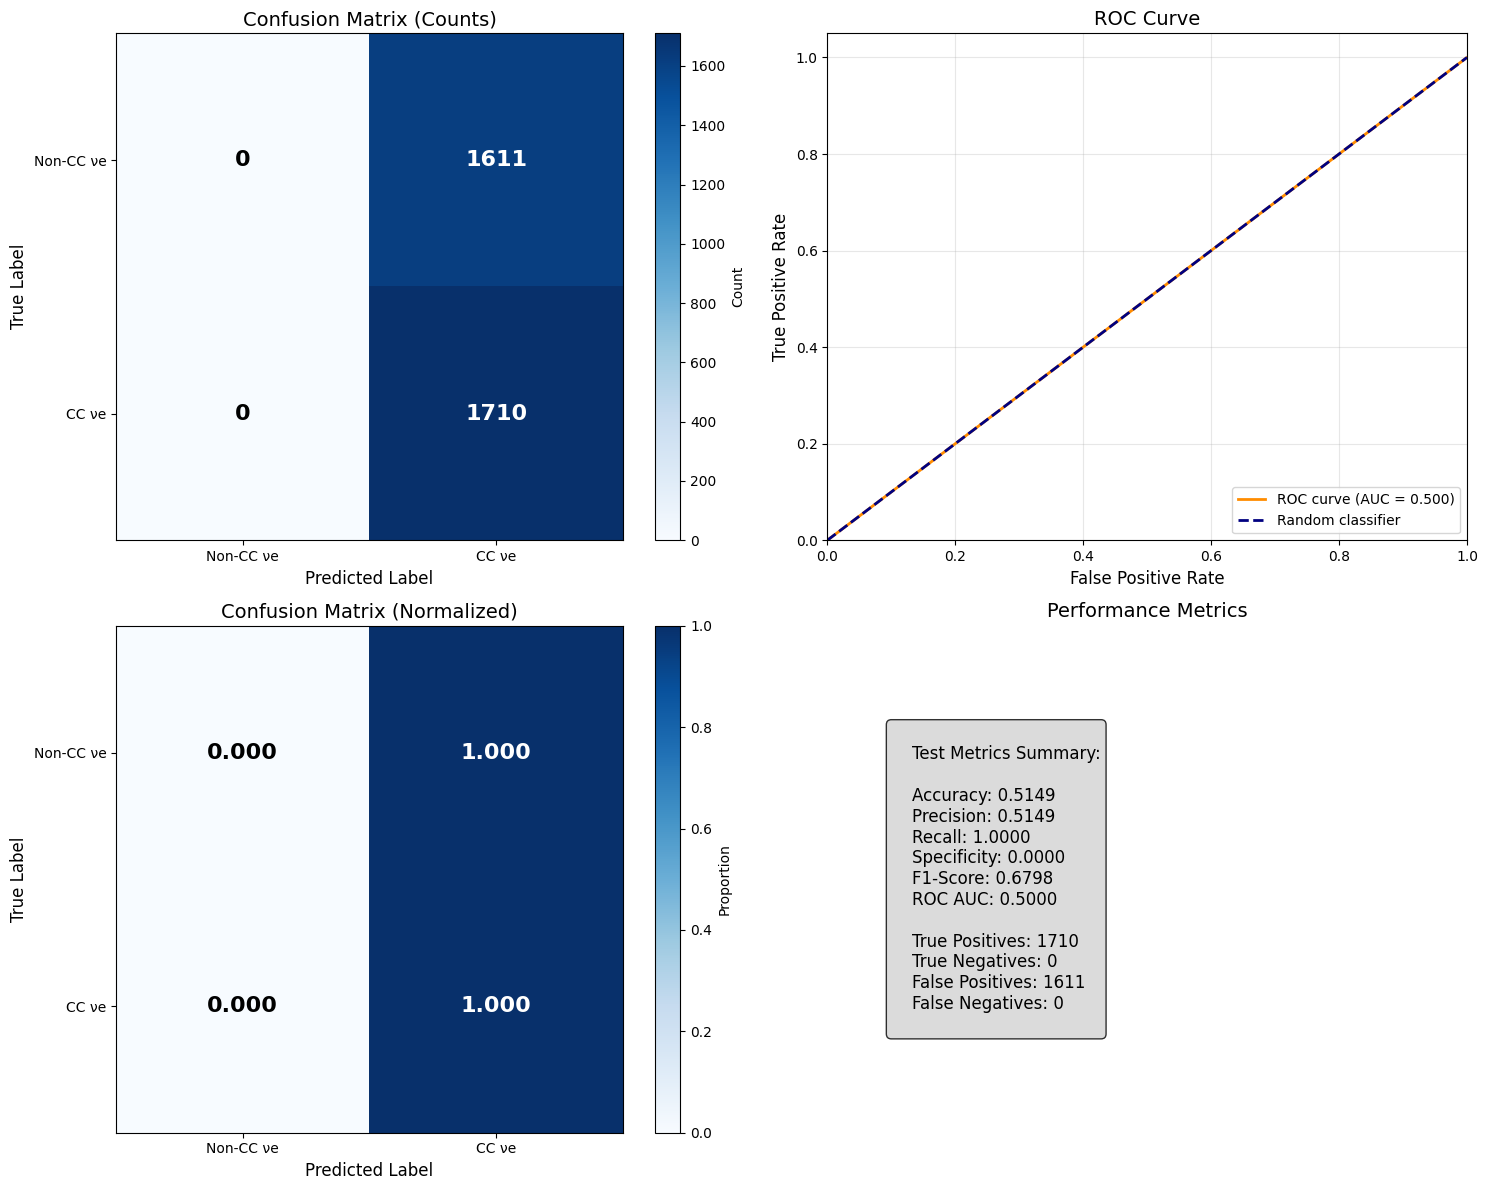
\includegraphics[width=0.9\textwidth]{src/LeNET_1ch_top50_dataset_scale05.png}
%         % \caption{Caption for the first image}
%         \label{fig:Letop5005sub1}
%     \end{subfigure}
    
%     \vspace{1cm}
    
%     \begin{subfigure}{\textwidth}
%         \centering
%         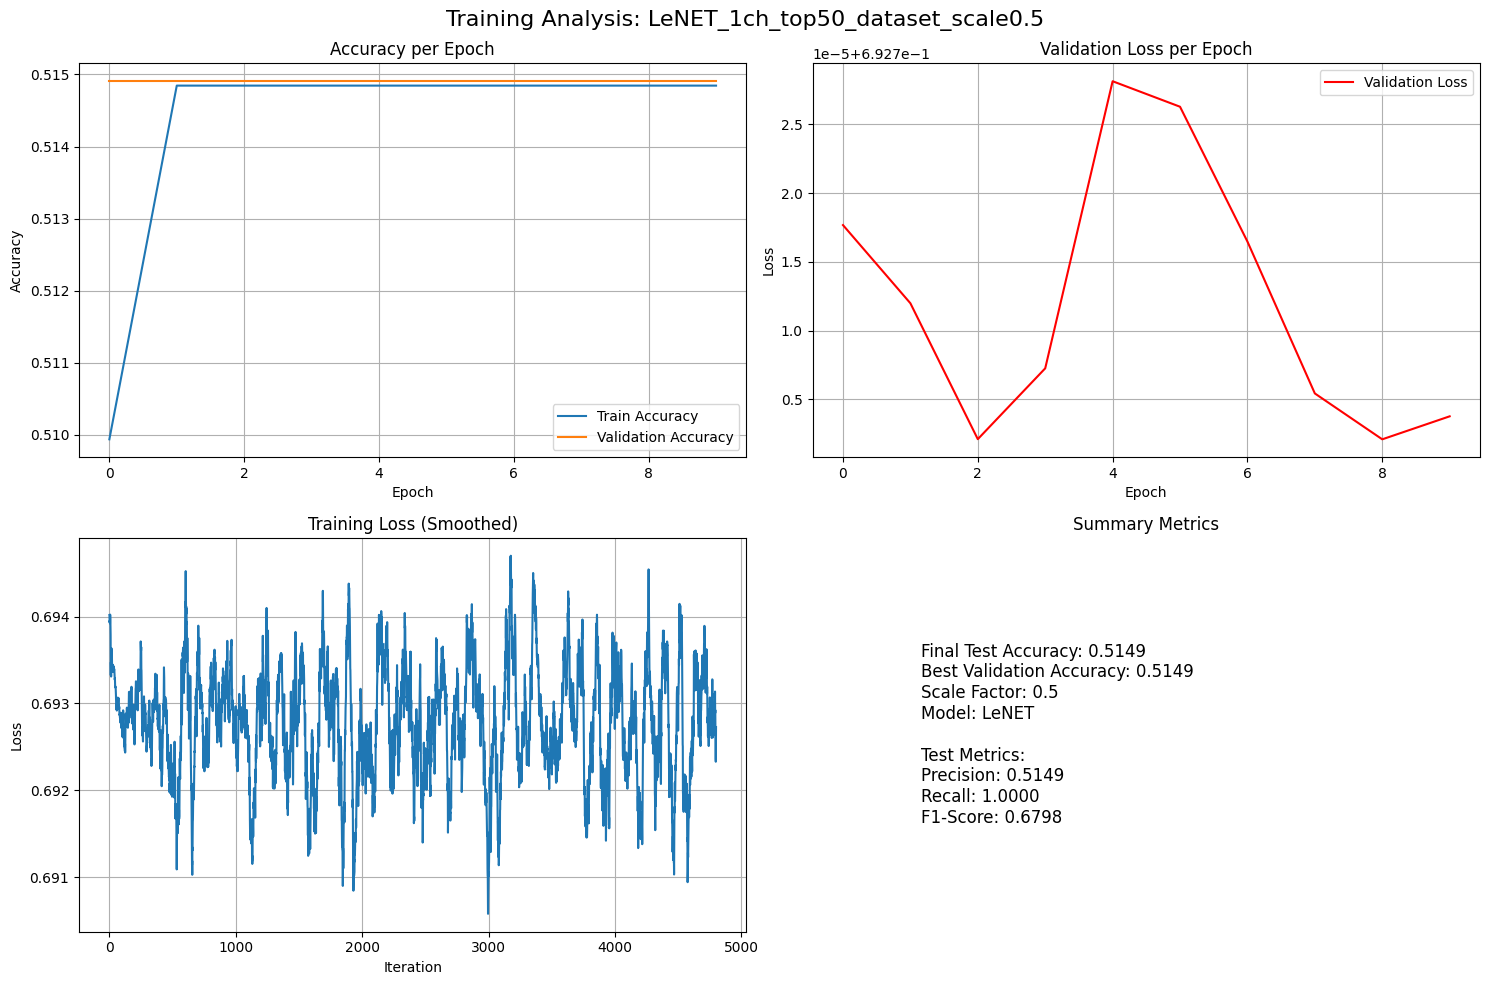
\includegraphics[width=0.9\textwidth]{src/LeNET_1ch_top50_dataset_scale05loss.png}
%         % \caption{Caption for the second image}
%         \label{fig:Letop5005sub2}
%     \end{subfigure}
%     \caption{LeNET training results on the top50 dataset with images scaled down to 0.5 of their original size.}
%     \label{fig:Letop5005stacked}
% \end{figure}

% \newpage

Best achieved training results for the LeNet-like network are presented in Figure \ref{fig:Letop5033stacked}. The network was unable to learn any meaningful features from the data, as evidenced by the fact that it classified all events as background events. The resulting ROC curve (Figure~\ref{fig:Lefull33sub1}) lies close to the diagonal, indicating that the classifier performs no better than random guessing. The training loss did not decrease and simply oscillated around a constant value. The classification accuracy remained close to 0.5 for all runs. It can be reasonably concluded that the network did not learn any non-trivial features from the data, and training was completely unsuccessful.

\subsection{AlexNet}

Training results for the AlexNet-like network are presented in Figures~\ref{fig:full33stacked}, \ref{fig:full5sub1}, \ref{fig:top5033stacked}, and \ref{fig:top5005stacked}. Overall, the network was able to achieve satisfactory results for all datasets and scaling factors. The performance metrics achieved for each training suggest that some non-trivial underlying patterns were learned by the network. Training loss behaved as expected—decreasing steadily, with the rate of change becoming smaller with each epoch. Classification accuracy increased over the course of training.

In all cases, AlexNet-based networks performed better at classifying non-CC events than CC events (the number of false positives in the latter case was greater in every training). Increasing the scale factor of the input image did increase the network's performance, but not in a very significant way. Most of the improvement came from reducing the number of false negatives for electron neutrino interactions.

\begin{figure}[H]
    \centering
    \begin{subfigure}{\textwidth}
        \centering
        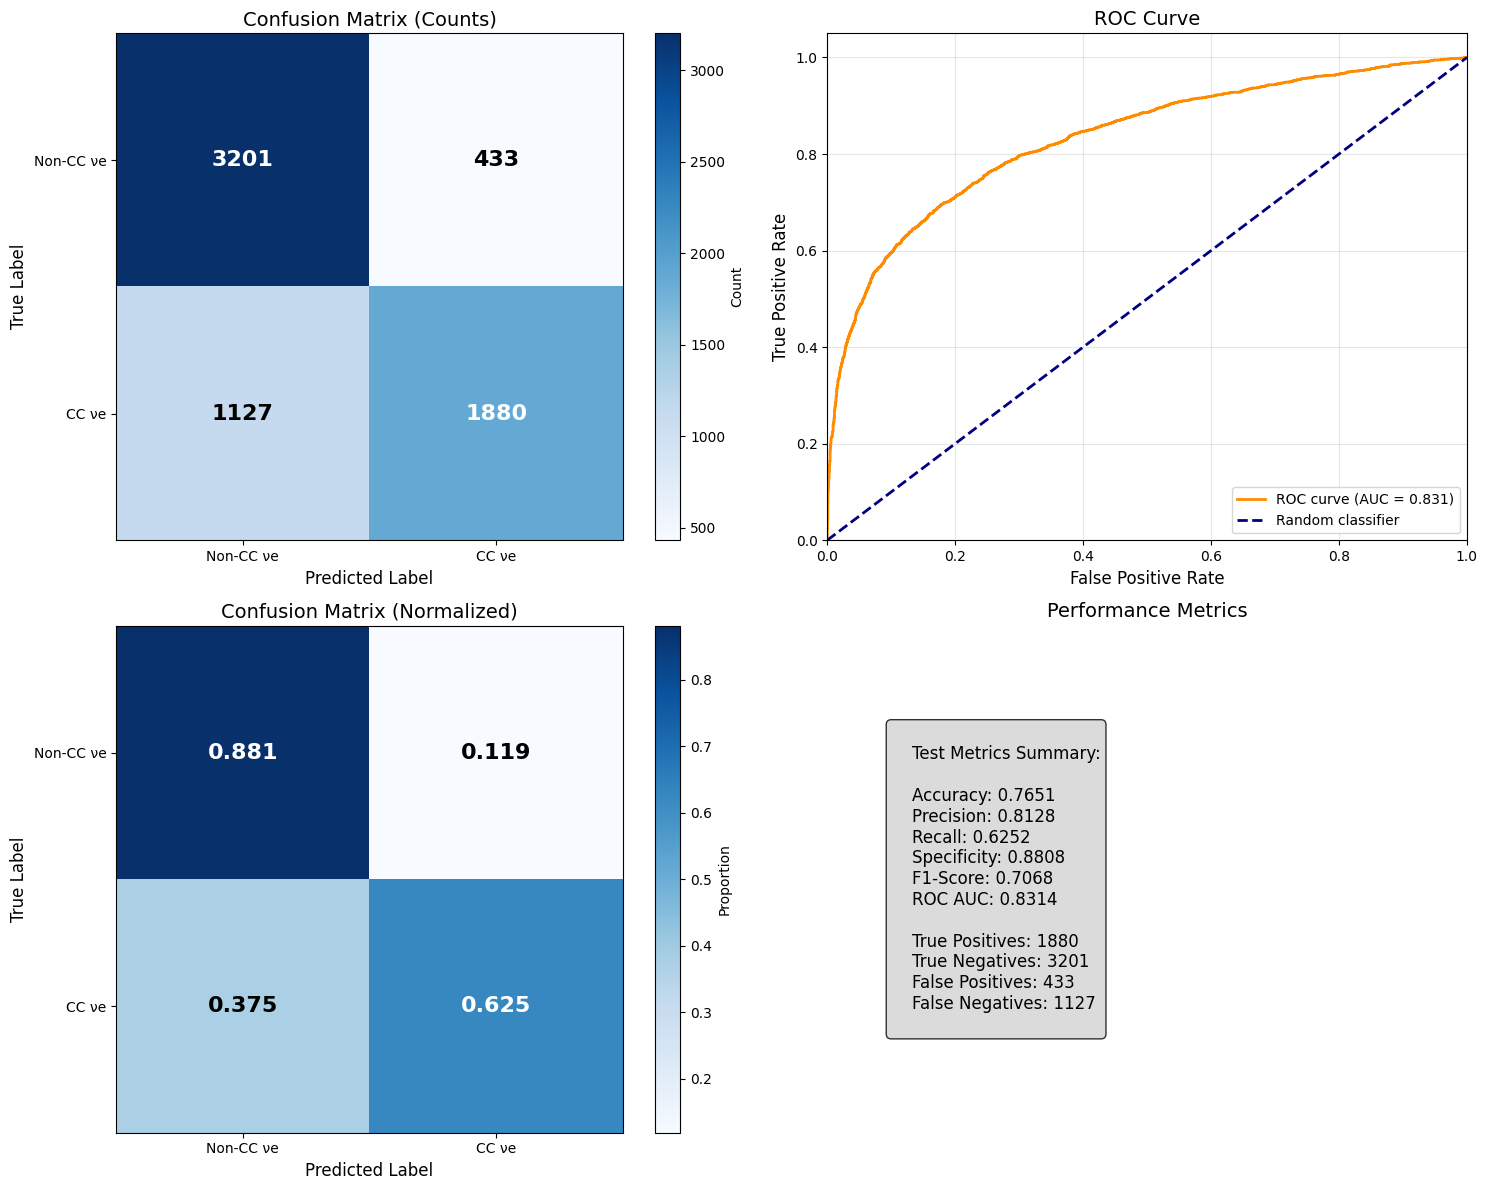
\includegraphics[width=0.9\textwidth]{src/AlexCNN_1ch_full_dataset_scale033.png}
        % \caption{Caption for the first image}
        \label{fig:full33sub1}
    \end{subfigure}
    
    \vspace{1cm}
    
    \begin{subfigure}{\textwidth}
        \centering
        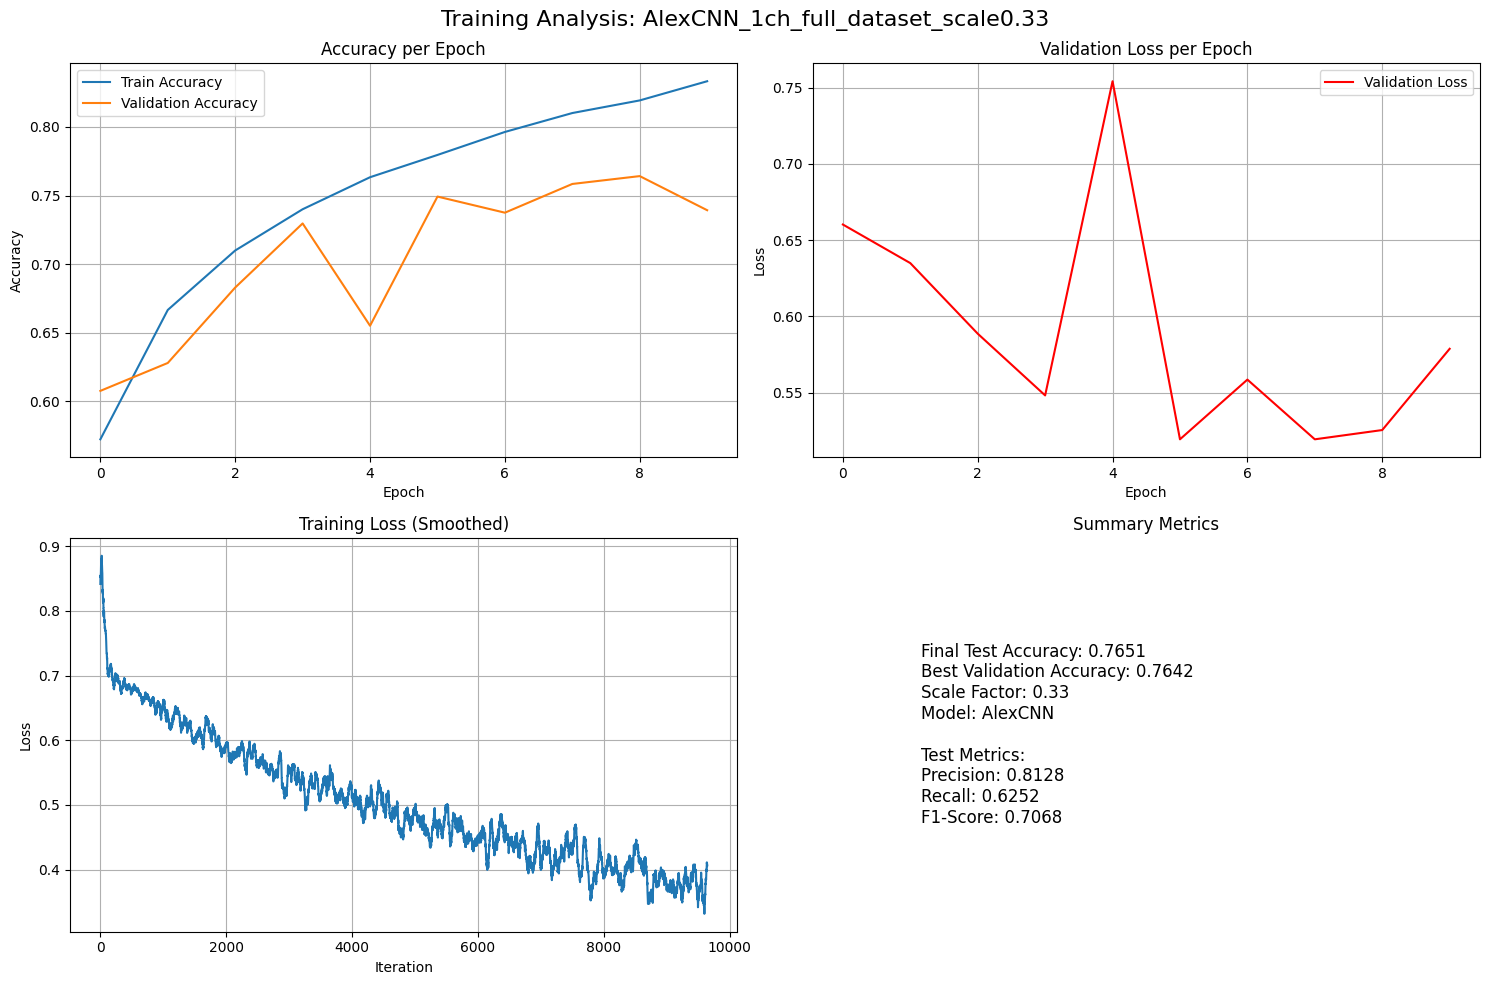
\includegraphics[width=0.9\textwidth]{src/AlexCNN_1ch_full_dataset_scale0.33loss.png}
        % \caption{Caption for the second image}
        \label{fig:full33sub2}
    \end{subfigure}
    \caption{Alexnet training results on the full dataset with images scaled down to 0.33 of their original size.}
    \label{fig:full33stacked}
\end{figure}

\newpage

\begin{figure}[H]
    \centering
    \begin{subfigure}{\textwidth}
        \centering
        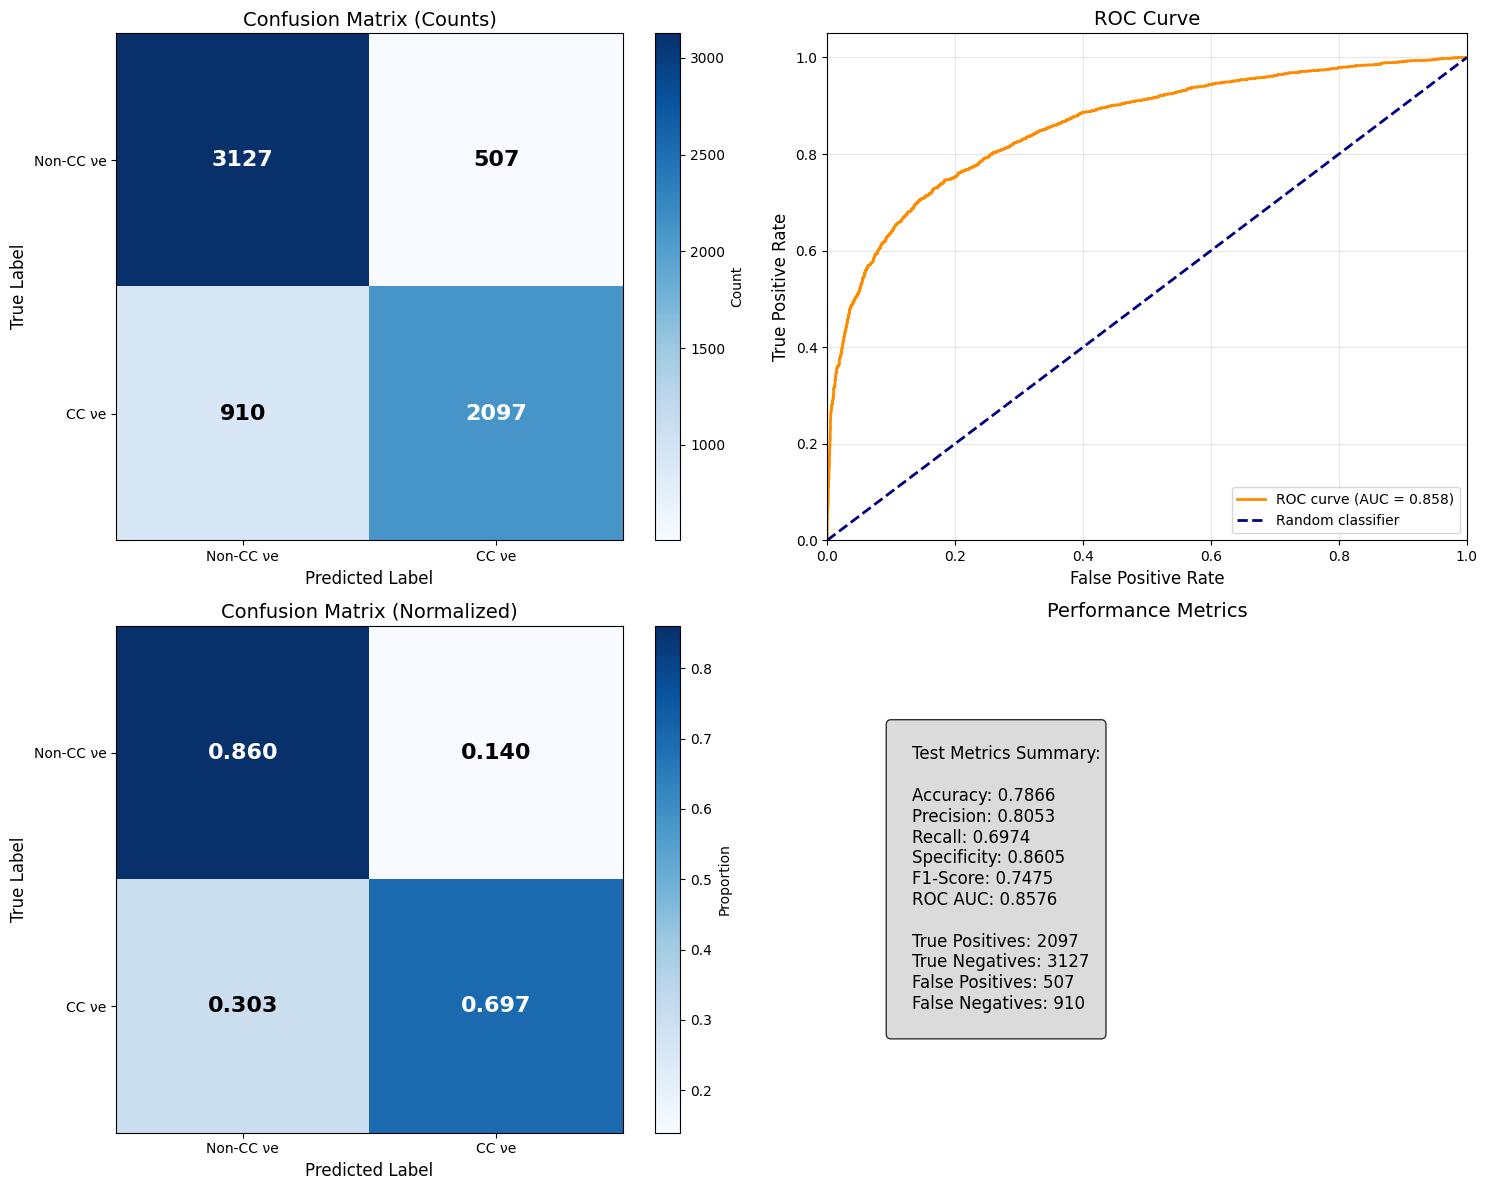
\includegraphics[width=0.9\textwidth]{src/AlexCNN_1ch_full_dataset_scale05.png}
        % \caption{Caption for the first image}
        \label{fig:full5sub1}
    \end{subfigure}
    
    \vspace{1cm}
    
    \begin{subfigure}{\textwidth}
        \centering
        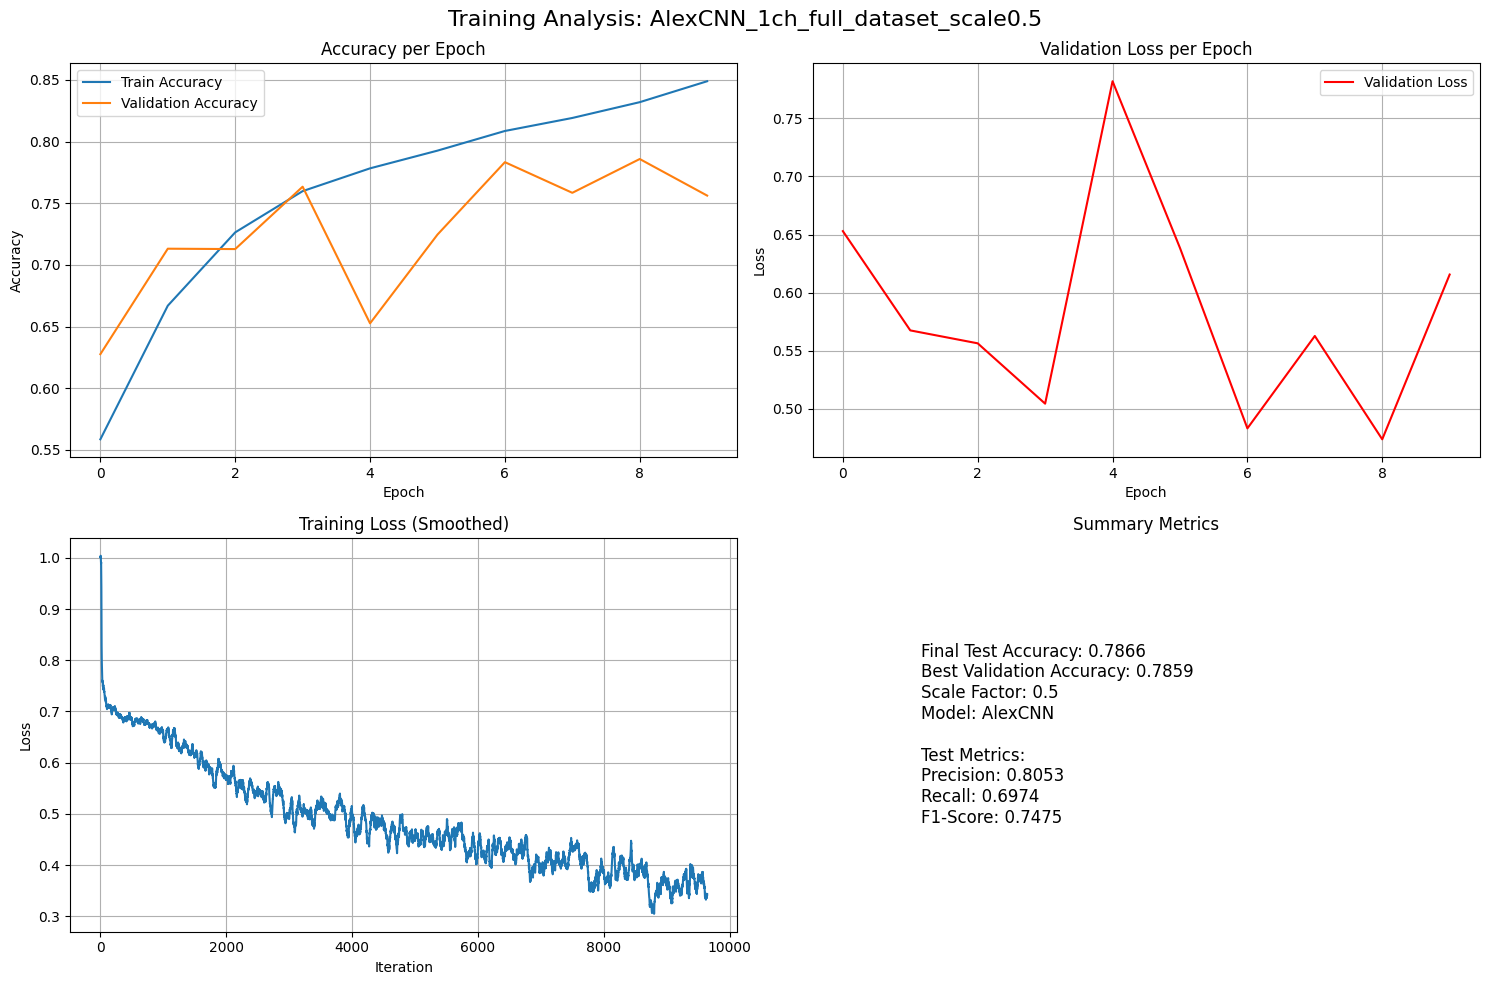
\includegraphics[width=0.9\textwidth]{src/AlexCNN_1ch_full_dataset_scale05loss.png}
        % \caption{Caption for the second image}
        \label{fig:full5sub2}
    \end{subfigure}
    \caption{Alexnet training results on the full dataset with images scaled down to 0.5 of their original size.}
    \label{fig:full5stacked}
\end{figure}

\newpage

\begin{figure}[H]
    \centering
    \begin{subfigure}{\textwidth}
        \centering
        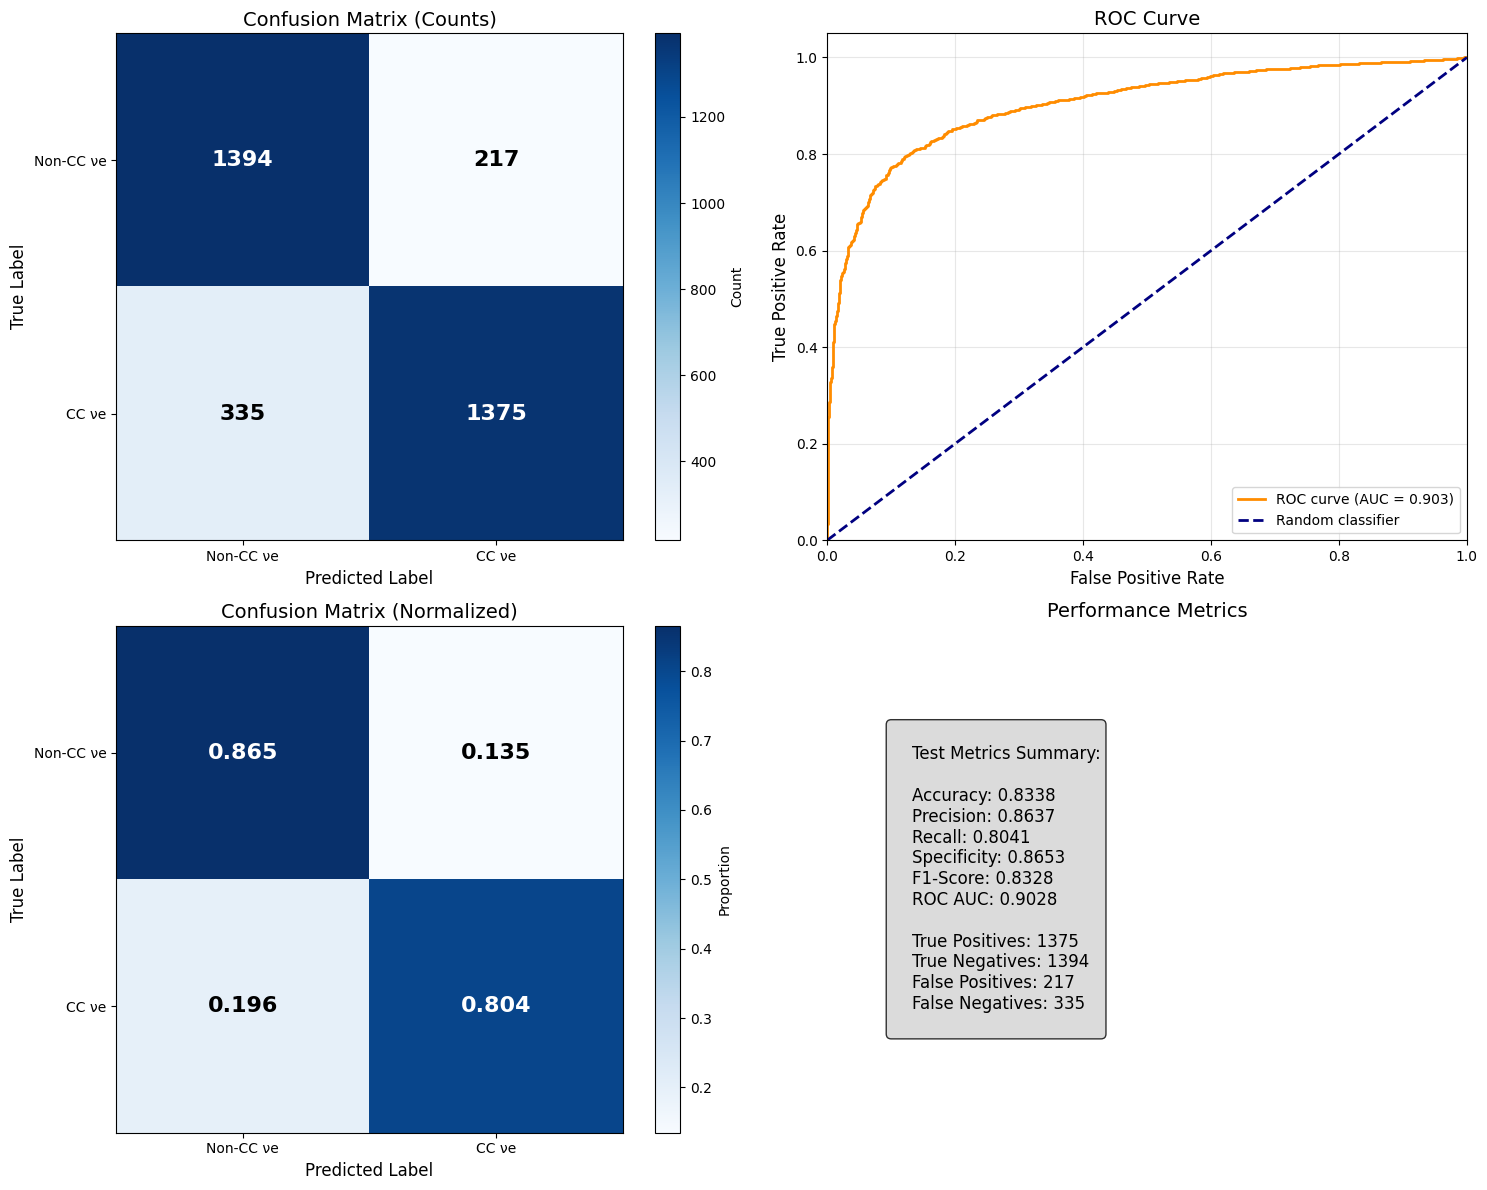
\includegraphics[width=0.9\textwidth]{src/AlexCNN_1ch_top50_dataset_scale033.png}
        % \caption{Caption for the first image}
        \label{fig:top5033sub1}
    \end{subfigure}
    
    \vspace{1cm}
    
    \begin{subfigure}{\textwidth}
        \centering
        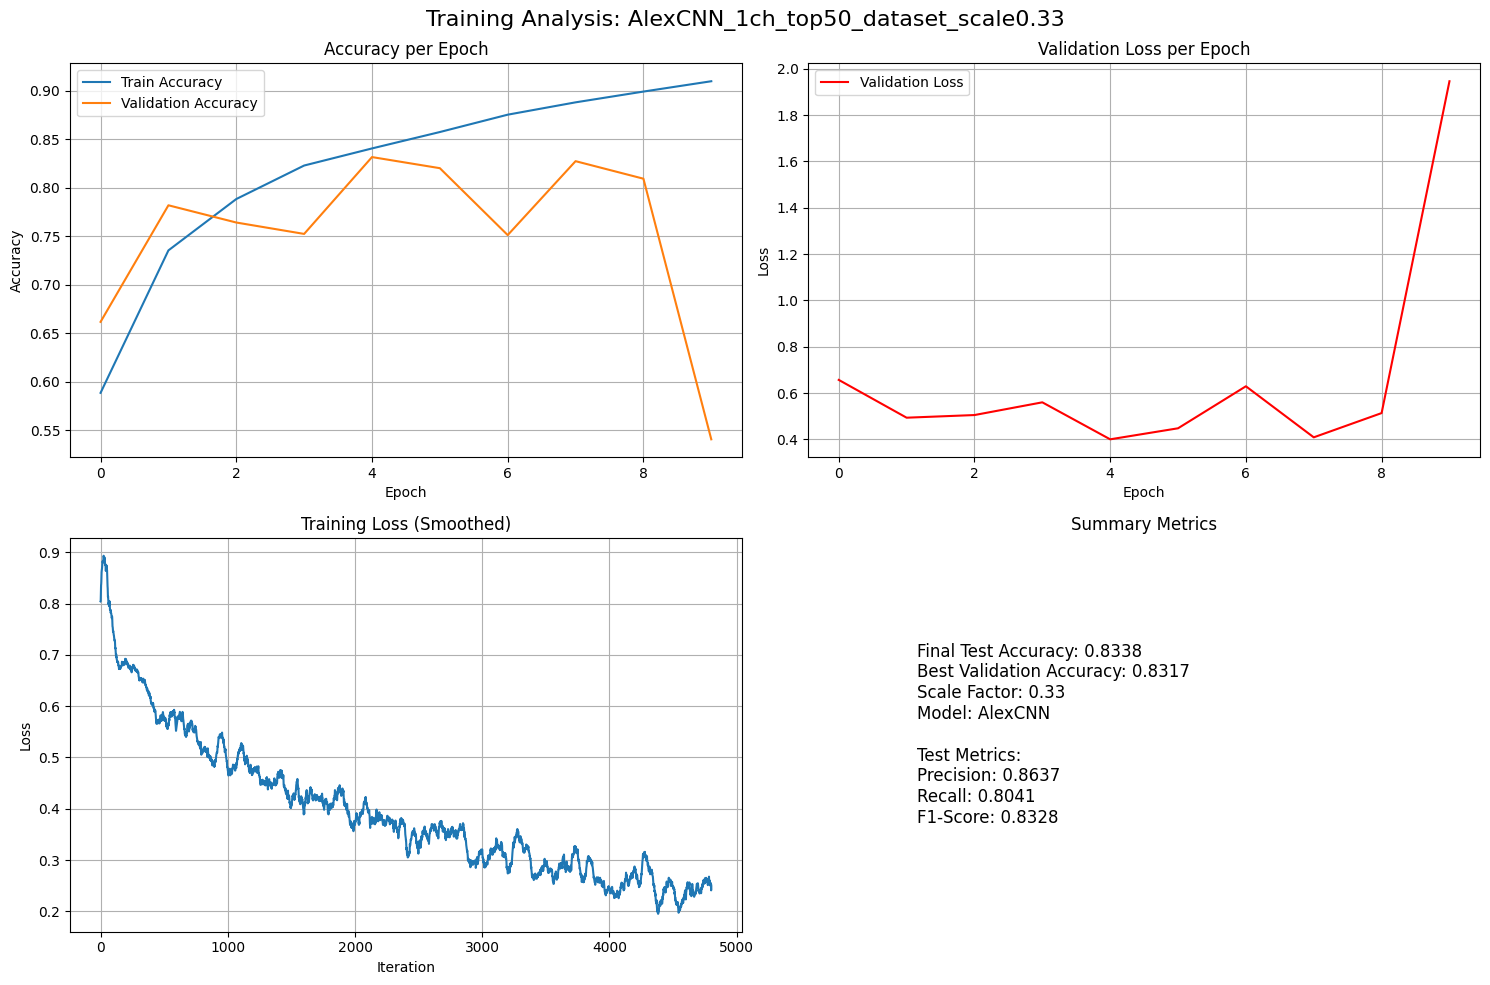
\includegraphics[width=0.9\textwidth]{src/AlexCNN_1ch_top50_dataset_scale033loss.png}
        % \caption{Caption for the second image}
        \label{fig:top5033sub2}
    \end{subfigure}
    \caption{Alexnet training results on the top50 dataset with images scaled down to 0.33 of their original size.}
    \label{fig:top5033stacked}
\end{figure}

\newpage

\begin{figure}[H]
    \centering
    \begin{subfigure}{\textwidth}
        \centering
        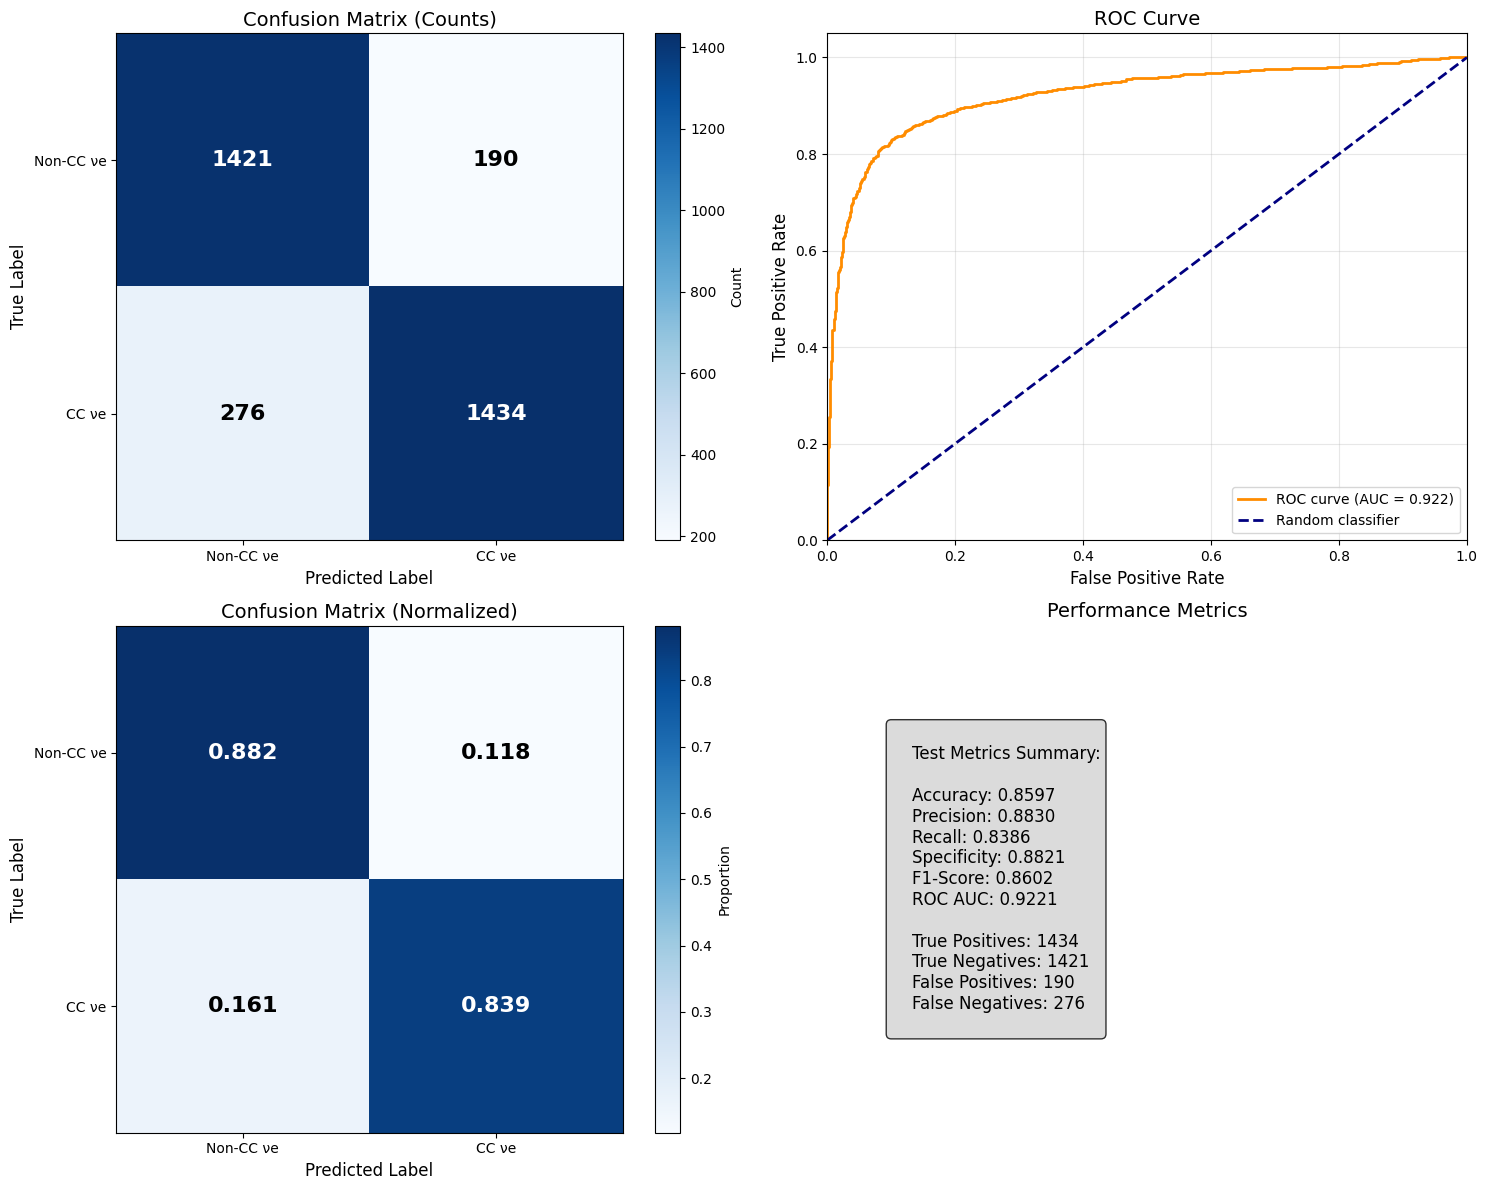
\includegraphics[width=0.9\textwidth]{src/AlexCNN_1ch_top50_dataset_scale0.5.png}
        % \caption{Caption for the first image}
        \label{fig:top5005sub1}
    \end{subfigure}
    
    \vspace{1cm}
    
    \begin{subfigure}{\textwidth}
        \centering
        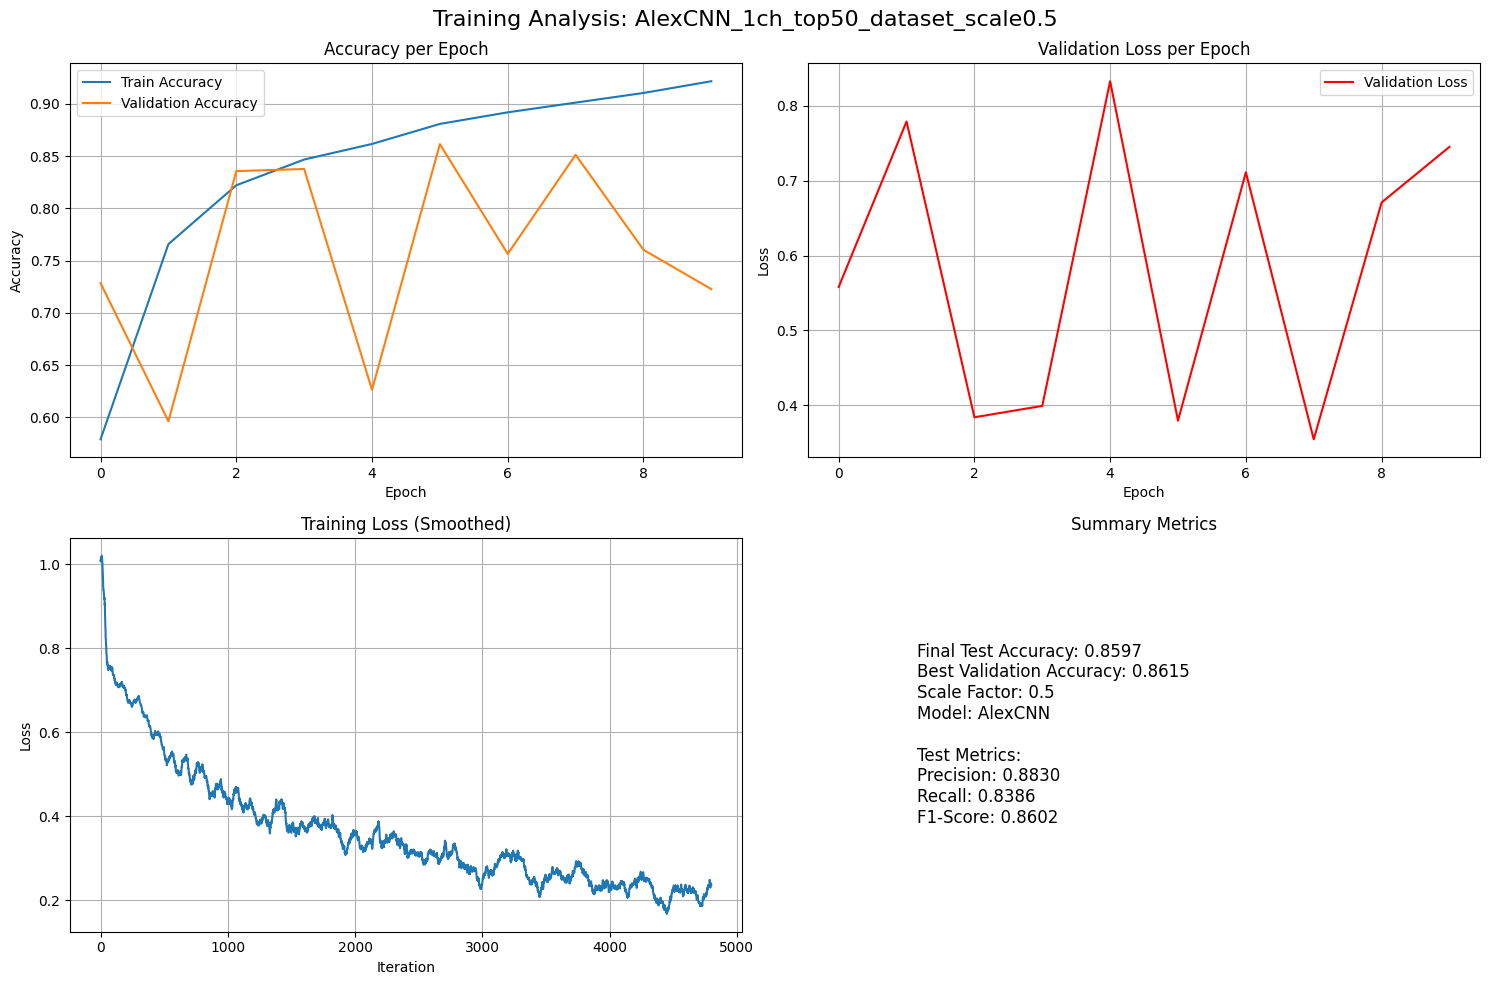
\includegraphics[width=0.9\textwidth]{src/AlexCNN_1ch_top50_dataset_scale05losses.png}
        % \caption{Caption for the second image}
        \label{fig:top5005sub2}
    \end{subfigure}
    \caption{Alexnet training results on the top50 dataset with images scaled down to 0.5 of their original size.}
    \label{fig:top5005stacked}
\end{figure}

\newpage

\subsection{discussion}

As noted before, the LeNet-like network was unable to learn any meaningful features from the data, while the AlexNet-like network performed relatively well on all datasets. This outcome could have been somewhat expected, as LeNet is significantly less complex and shallower than AlexNet, which limits its ability to learn complex features from the data. It may be possible that the learning results could be improved by adjusting the training parameters, but the complete lack of performance suggests that it is not well-suited for the classification task at hand.

\begin{figure}[H]
    \centering
    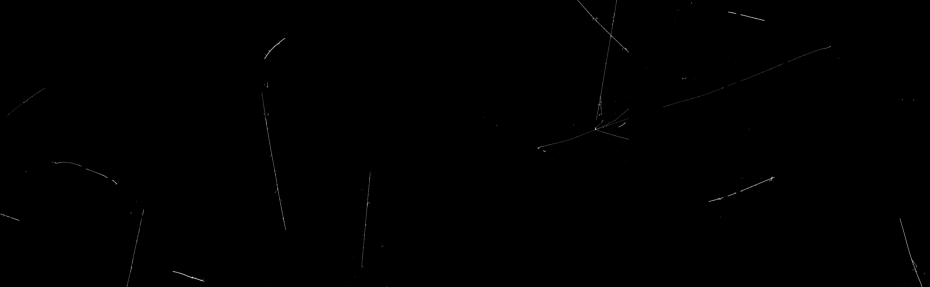
\includegraphics[width=0.8\textwidth]{src/without_flag_20.png}
    \caption{Example of a wire readout image where no neutrino interaction is present, yet AlexNet-Like network classified it as a charged-current (CC) event.}
    \label{fig:without_flag}
\end{figure}

The strong performance of the AlexNet-like network suggests that it was able to learn some non-trivial features from the data.  The fact that the network ended up being slightly better at classifying non-CC events than CC events can also be considered expected behavior—certain noise patterns (such as the presence of tracks from other leptons or overlapping noise tracks) may be misinterpreted as electron showers\ref{fig:without_flag}. The performance of the network could still be improved by refining the training parameters, but the observed rise in validation loss during later training epochs suggests that the network may have started to overfit the training data. Training on a larger dataset could potentially bring a meaningful performance increase.

Taking into account the high accuracy of the AlexNet-like network, it can be reasonably assumed that the classification problems, as previously stated, are solvable using deep learning techniques. To extend the discussion, another approach to image classification was attempted—namely, one involving an image transformer architecture. The details of this approach are described in the next chapter.

\chapter{Transformer}

The transformer is a deep learning architecture introduced for processing sequential data\cite{Vaswani2017Attention}. Unlike convolutional neural networks (CNNs), which use local receptive fields to capture spatial features, Transformers attend to the entire input sequence simultaneously.

The core components of the Transformer include multi-head self-attention layers, residual connections, and layer normalization. The architecture is composed of repeated encoder blocks, each consisting of an attention sublayer followed by a deep neural network and normalization components (see Figure~\ref{fig:transformerEncoder}).

Transformer architecture was adapted to later works to a number of tasks, including image classification \cite{ViT}. In this chapter, applications of these adaptations will be explored.

Inputs to the transformer are first passed through an embedding layer, and positional encodings are added to the embeddings to retain information about the order of tokens in the sequence. These embeddings are then passed through a number of encoder blocks, each consisting of multi-head self-attention and linear layers, with the output of one block serving as the input to the next. The final output is a sequence of continuous vectors, which can then be processed by a decoder or used directly for tasks such as classification or regression.



\section{Elements of the Transformer Architecture}

\subsection{Embeddings}

\subsubsection{general mechanism}

\begin{figure}[h]
    \centering
    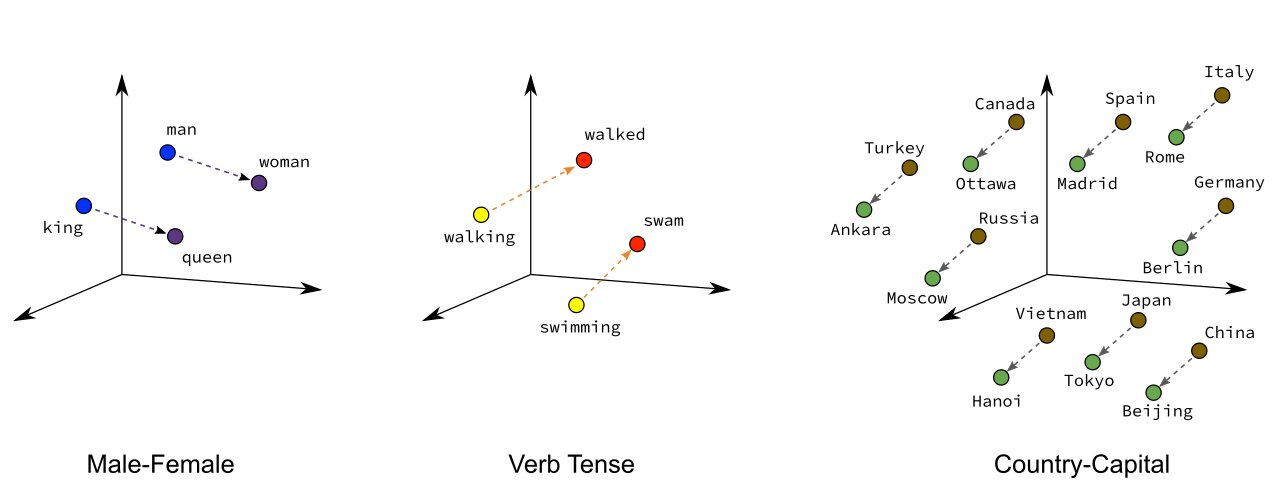
\includegraphics[width=0.9\textwidth]{src/word_embeddings_semantics.png}
    \caption{A simplified example of word embeddings projected into three dimensions. Words that share functional or structural roles—such as verb tense or country-capital pairs—tend to form consistent spatial patterns\cite{CloudxLabEmbeddings}.}
    \label{fig:embedding_example}
\end{figure}

Transformer-based architectures operate on continuous vector representations. For this reason, each input passed into the network—also known as a token—must be mapped to a fixed-dimensional dense vector, known as an embedding. An example of word embeddings in a low-dimensional space is shown in Figure\ref{fig:embedding_example}.

Formally, for an input consisting of \( V \) tokens and an embedding dimension \( d \), the embedding layer is represented by a matrix \( \mathbf{E} \in \mathbb{R}^{V \times d} \).

Given a sequence of input tokens \( \{t_1, t_2, \ldots, t_n\} \), the corresponding embedding vectors \( \{\mathbf{x}_1, \ldots, \mathbf{x}_n\} \) are obtained by indexing into the embedding matrix:
\[
\mathbf{x}_i = \mathbf{E}[t_i] \in \mathbb{R}^d
\]

The embedding matrix consists of trainable parameters and is optimized jointly with the rest of the model. The goal of this mapping is to project discrete inputs into a continuous space where meaningful relationships can be learned during training.

\subsubsection{Positional encoding}

\begin{figure}[H]
    \centering
    \begin{minipage}{0.8\textwidth}
        \centering
        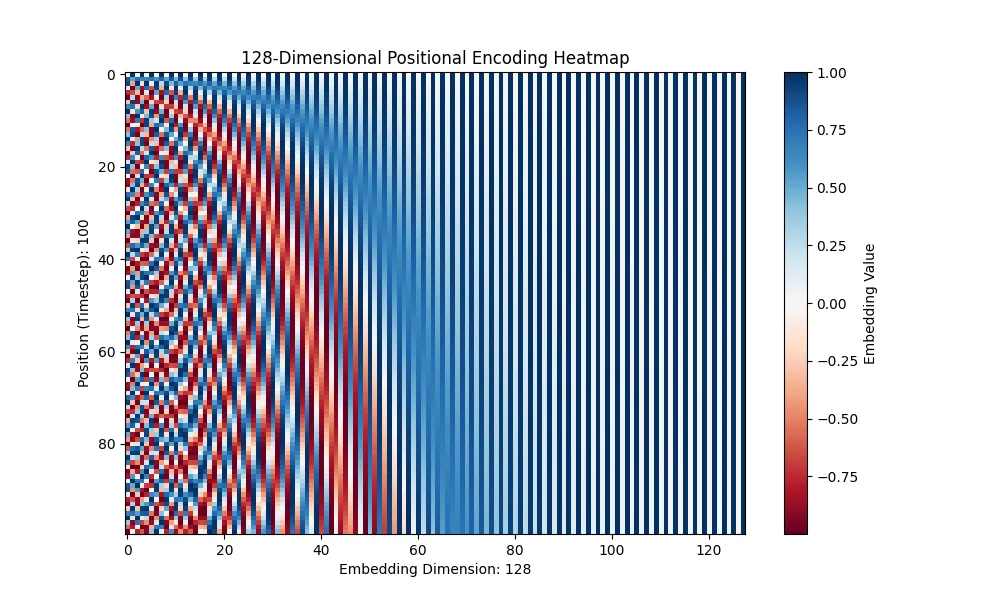
\includegraphics[width=\textwidth]{src/embedings.png}
    \end{minipage}
    \vspace{0.2cm}
    \begin{minipage}{0.7\textwidth}
        \centering
        \begin{align*}
        PE(pos, 2i) &= \sin\left(\frac{pos}{10000^{\frac{2i}{d_{\text{model}}}}}\right) \\
        PE(pos, 2i + 1) &= \cos\left(\frac{pos}{10000^{\frac{2i}{d_{\text{model}}}}}\right)
        \end{align*}
    \end{minipage}
    \label{fig:positionalEncoding}
    \caption{Example of how positional encoding can be handled. The heatmap at the top visually represents a positional encoding for 128-dimensional vectors. Each row corresponds to a position in the input sequence, and each column represents a dimension within the embedding vector. The color gradient signifies the value of the positional encoding at that specific position and dimension. The equations at the bottom define the sinusoidal functions used to compute the positional encoding for each position \( pos \) and dimension \( i \) in the embedding vector.\cite{Kubo2024Transformer}}
\end{figure}

The sinusoidal positional encoding and its heatmap representation are shown in the diagram in Figure~\ref{fig:positionalEncoding}.

Importantly, the process described in the previous section does not inherently retain positional information of the input sequence. To address this, transformers incorporate positional encoding, which injects information about the position of each token in the sequence into the input embeddings. The encoded position of each token is added to its corresponding embedding before being passed through the transformer layers:
\[
\mathbf{z}_0 = \mathbf{x} + \mathbf{P}
\]
where \( \mathbf{x} \) denotes the input embedding and \( \mathbf{P} \) is the positional encoding.


\subsection{Transformer Encoder}

Encoder blocks serve as the fundamental building blocks of transformers. Inputs of each block have the same dimensionality as the outputs, making it possible to stack these block one aster another. The general hope is that each such block will encode some learned information about the relationships between embedded input tokens into its output.

\subsubsection{Attention}

\begin{figure}[h]
    \centering
    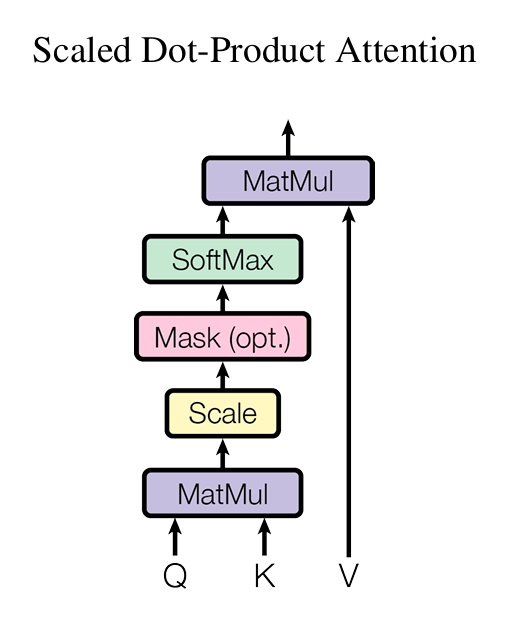
\includegraphics[width=0.4\textwidth]{src/scaledDotProd.png}
    \caption{Graphic representation of a single attention head. The input query, key, and value matrices are passed through a scaled dot-product attention mechanism, which computes attention scores and produces the output.\cite{Vaswani2017Attention}}
    \label{fig:singleAttentionHead}
\end{figure}

Attention is a central component of the transformer architecture, as well as the encoder block. It enables the model to extract relationships between different parts of the embedded input sequences. This mechanism is implemented through structures known as attention heads, which are illustrated in Figure~\ref{fig:singleAttentionHead}. Each attention head receives three inputs: the query matrix \( Q \in \mathbb{R}^{n \times d_k} \), the key matrix \( K \in \mathbb{R}^{n \times d_k} \), and the value matrix \( V \in \mathbb{R}^{n \times d_v} \), where \( n \) denotes the sequence length, and \( d_k \), \( d_v \) are the dimensionalities of the key and value vectors, respectively. The attention computation begins with calculating a score matrix by taking the dot product of the query and the transpose of the key: 
\[
\text{scores} = QK^\top
\]
These scores are then scaled by the inverse square root of the key dimension and passed through a softmax function to obtain normalized attention weights:
\[
\text{weights} = \text{softmax}\left(\frac{\text{scores}}{\sqrt{d_k}}\right)
\]
Finally, these weights are used to compute a weighted sum of the value vectors, resulting in the output of the attention head:
\[
\text{Attention}(Q, K, V) = \text{weights} \cdot V
\]

\subsubsection{Multi-head attention}

\begin{figure}[h]
    \centering
    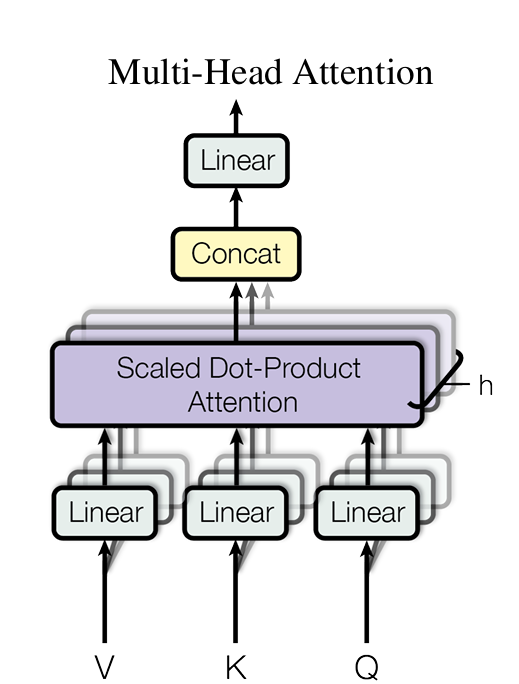
\includegraphics[width=0.4\textwidth]{src/multiHead.png}
    \caption{Graphic representation of a multi-head attention mechanism. The input query, key, and value matrices are passed through multiple independent attention heads, each computing its own attention output. The outputs of all heads are concatenated and projected back to the original dimensionality\cite{Vaswani2017Attention}.}
    \label{fig:multiHeadAttention}
\end{figure}

The multi-head attention mechanism extends the single-head idea by introducing multiple independent attention heads. Before attention is computed, the original input matrices \( Q \), \( K \), and \( V \) are each passed through separate trainable linear projections.

Instead of applying a single attention function with \( d_{\text{model}} \)-dimensional queries, keys, and values, the multi-head attention mechanism projects the inputs into multiple lower-dimensional subspaces and performs attention in parallel across these subspaces.

Specifically, for each attention head \( i \in \{1, \dots, h\} \), the queries \( Q \), keys \( K \), and values \( V \) are linearly projected using trainable weight matrices:
\[
QW_i^Q \in \mathbb{R}^{n \times d_k}, \quad KW_i^K \in \mathbb{R}^{n \times d_k}, \quad VW_i^V \in \mathbb{R}^{n \times d_v}
\]
Each attention head computes scaled dot-product attention independently:
\[
\text{head}_i = \text{Attention}(QW_i^Q, KW_i^K, VW_i^V)
\]

The outputs of all attention heads are then concatenated along the feature dimension:
\[
\text{MultiHead}(Q, K, V) = \text{Concat}(\text{head}_1, \ldots, \text{head}_h)W^O
\]
where \( W^O \in \mathbb{R}^{hd_v \times d_{\text{model}}} \).

The matrices \( W^Q_i \), \( W^K_i \), \( W^V_i \), and \( W^O \) consist of trainable parameters optimized during training.

A visual overview of the multi-head attention mechanism is provided in Figure~\ref{fig:multiHeadAttention}.

\subsubsection{Residual connections and layer normalization}

\begin{figure}[h]
    \centering
    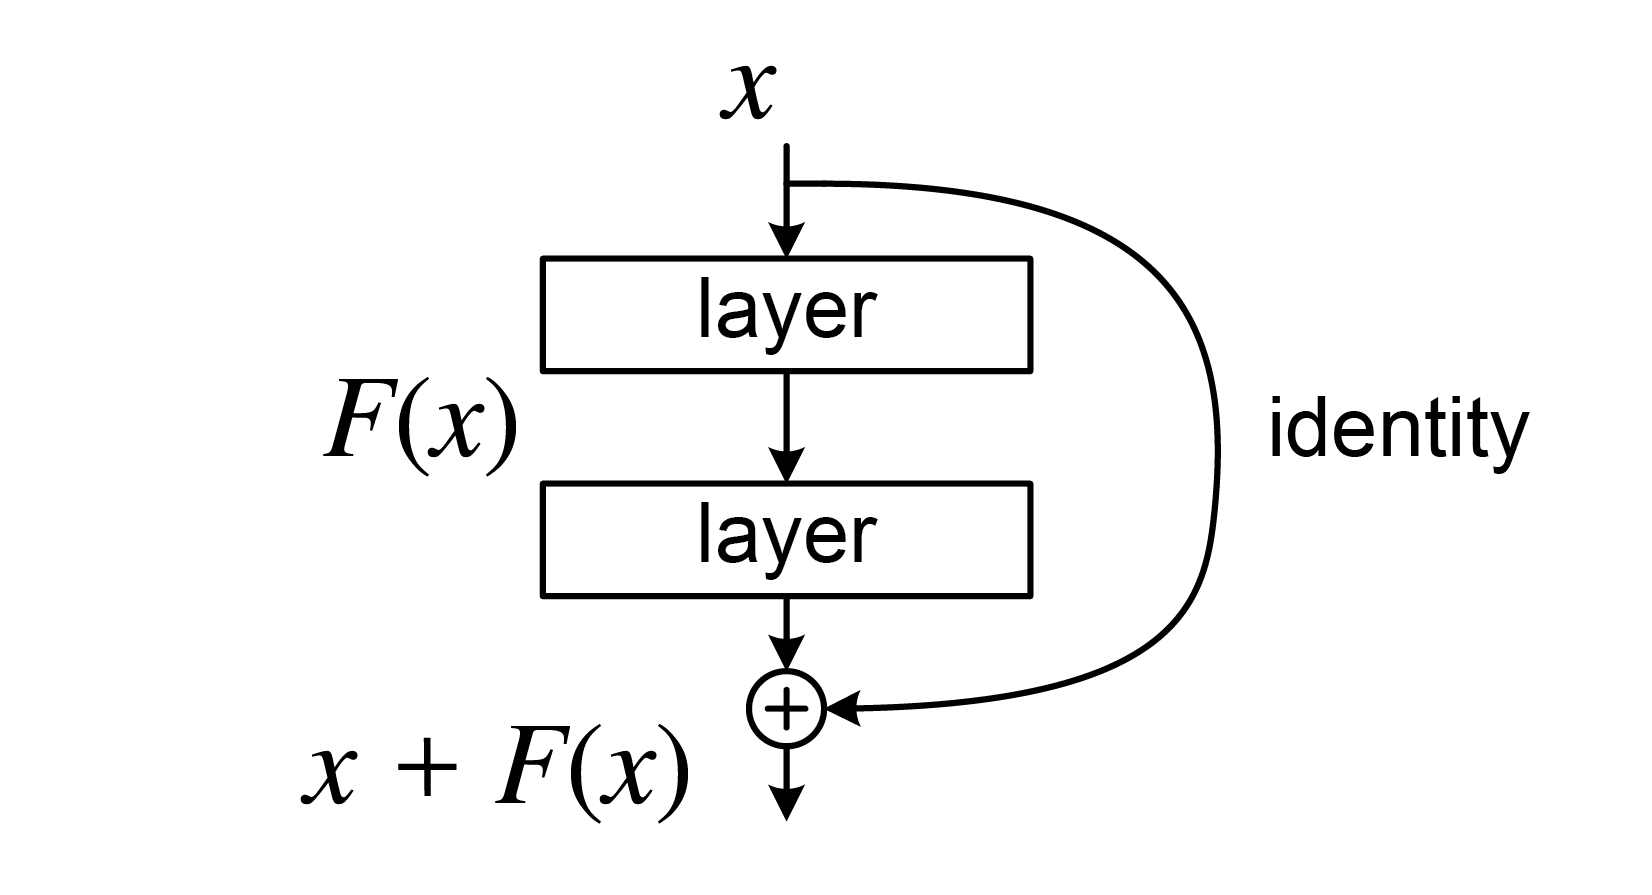
\includegraphics[width=0.5\textwidth]{src/ResBlock.png}
    \caption{Graphic representation of a residual connection\cite{resConn}.}
    \label{fig:resCon}
\end{figure}

In order to stabilize learning Transformers commonly apply residual connections around some of their sublayers.

These connections, when given an input \( \mathbf{x} \) and a sublayer function \( \text{Sublayer}(\cdot) \), compute the output as:
\[
\text{LayerNorm}(\mathbf{x} + \text{Sublayer}(\mathbf{x}))
\]

\ref{fig:resCon}

Implementation of these layers was empirically shown to improve convergence and performance of the model.


\subsubsection{Full transformer block}

\begin{figure}[h]
    \centering
    \includegraphics[width=0.5\textwidth]{src/transformerBlockSingle.pdf}
    \caption{Visual representation of a transformer block. \cite{transformerBlockSingle}}
    \label{fig:transformerEncoder}
\end{figure}

Each encoder block consists of a multi-head attention mechanism, the outputs of which are then passed through a neural network—both of which are wrapped in residual connections (see Figure~\ref{fig:transformerEncoder}).

\subsection{Full Transformer} 

\begin{figure}[h]
    \centering
    \includegraphics[width=0.17\textwidth]{src/transformerEncoder.pdf}
    \caption{Visual representation of a full transformer. \cite{Vaswani2017Attention}}
    \label{fig:transformerEncoder}
\end{figure}

Inputs to the transformer are first passed through an embedding layer, and positional encodings are added to the embeddings. These embeddings are then passed through a number of encoder blocks, with the output of one block serving as the input to the next.

General hope is that during training, each such block will encode some learned information about the relationships between embedded input tokens into its output, with each block progressively refining the representation of the input sequence.

The final output is a sequence of continuous vectors, which can then be processed by a decoder or used directly for tasks such as classification or regression.

\section{Image Transformer}

\subsection{Image Transformer Architecture}

The image transformer extends the standard transformer architecture to process visual inputs, originally proposed in \cite{ViT}. Rather than operating on word tokens, the input image is divided into a sequence of fixed-size non-overlapping patches. A typical configuration involves splitting the image into 16 patches of \(16 \times 16\) pixels each. 

\subsubsection{Classification Token}

To enable image-level classification, a special token known as the classification token, or [CLS] token, is prepended to the sequence of patch embeddings \ref. This token does not represent any specific region of the image and is initialized as a trainable vector. Throughout the transformer layers, it interacts with other tokens via the attention.

The general hope is that though these interactions it will gradually aggregate global information about the entire image. The [CLS] token is trained jointly with the model to optimize performance on the target classification task.

\subsubsection{Positional Encoding for image patches}

\begin{figure}[h]
    \centering
    \includegraphics[width=0.4\textwidth]{src/imNetEncodings.pdf}
    \caption{Cosine similarity of positional encoding for image patches from the original Vision Transformer paper. Embeddings for patches close to each other are similar\cite{ViT}.}
    \label{fig:imNetEncodings}
\end{figure}

To retain spatial context after converting image patches into a sequence, positional embeddings are added to each patch embedding. These embeddings are learnable parameters and are optimized during training alongside the rest of the model. Their purpose is to encode the location of each patch within the original image, enabling the model to distinguish between otherwise identical patches in different positions.

These embedding can either learned during training or be computed outright. Empirical analysis has shown that when parameters of the embedding is allowed to train with the network they evolve such that neighboring patches in the image space tend to receive similar positional encodings. This spatial correlation helps the transformer capture local structure while also enabling long-range dependencies to be modeled across distant regions of the image.

Figure~\ref{fig:imNetEncodings} shows how positional encodings correlate spatially in image transformers.

\subsubsection{Full Image Transformer}

\begin{figure}[H]
    \centering
    \includegraphics[width=0.7\textwidth]{src/visNet.pdf}
    \caption{Visual transformer architecture visualized\cite{ViTFUllGraph}}
    \label{fig:visNetArch}
\end{figure}

Input images are first divided into patches, which are then flattened and linearly projected to a fixed embedding dimension. Each patch embedding is augmented with a positional encoding to retain spatial information. The sequence of patch embeddings, along with the [CLS] token, is then passed through a stack of transformer encoder layers.

After processing through all transformer layers, the final output corresponding to the [CLS] token is treated as a global representation of the image. This output is passed to a multi-layer perceptron (MLP) head to produce a final classification. 

The transformer architecture adapted for images is illustrated in Figure~\ref{fig:visNetArch}.

\section{Transformer architecture used}

The specific transformer image transformer that ended up being used was largely based on the implementation kindly provided by professor Artur Kalinowski. Just like the one originally proposed in \cite{ViT} it divided images into patches of 16x16 pixels each. Each patch is mapped to a 32-dimensional embedding vector. Positional encoding is applied using sine and cosine functions across the embedding dimensions. The model includes a single multi-head self-attention layer with two heads to capture relationships between patches. A final three-layer multilayer perceptron consisted of layer sizes of 32, 16, and 2 neurons respectively.

\subsection{Training procedure}

This time, both the transformer itself as well as the training routine were implemented in tensorflow. For simplicity, the transformer only trained on the top50 dataset. Training was run for 10 epochs using a dataset split into training and validation batches. The validation set consisted of 1000 batches taken from the dataset, while the rest was used for training. An Adam optimizer with an exponentially decaying learning rate starting at 0.001 was used, with the learning rate decreasing by 5\% every 10 full passes through the training data. The model optimized a binary cross-entropy loss. Training incorporated early stopping, halting if the validation accuracy did not improve for 10 consecutive epochs.

\section{Transformer training results and evaluation}

\begin{figure}[H]
    \centering

    \begin{minipage}[t]{0.8\textwidth}
        \centering
        \includegraphics[width=\textwidth]{src/tranformerMatrixFinal.png}
        
        % \caption{Caption 3}
    \end{minipage}

    \vspace{1cm}

    \begin{minipage}[t]{0.48\textwidth}
        \centering
        \includegraphics[width=\textwidth]{src/transformerLoss.png}
        % \caption{Caption 1}
    \end{minipage}
    \hfill
    \begin{minipage}[t]{0.48\textwidth}
        \centering
        \includegraphics[width=\textwidth]{src/transformerROCurve.png}
        % \caption{Caption 2}
    \end{minipage}
    \caption{Transformer training results. The left image shows the normalized confusion matrix, the middle image shows the ROC curve, and the right image shows the training loss over epochs.}
    \label{fig:tranformerResults}
\end{figure}


\subsection{Training Summary}

Details of the training process are summarized in Figure~\ref{fig:tranformerResults}. The neural network was trained for 10 epochs using an exponentially decaying learning rate schedule. The final training loss reached 0.5839, with a training accuracy of 69.04\%. Validation performance at the end of training showed a loss of 0.6139 and an accuracy of 66.00\%, which was also the best recorded validation accuracy.

Testing on the held-out dataset yielded a final loss of 0.6218 and an accuracy of 66.03\%, indicating consistent generalization performance.

\subsection{Learning Dynamics}

During training, the loss decreased by 12.0\%, and accuracy improved by 9.75 percentage points. The training-validation accuracy gap was 3.04 percentage points, suggesting low overfitting. Loss fluctuations over the final five epochs were minimal (standard deviation: 0.0039), indicating moderate convergence.

\subsection{Classification Metrics}

\begin{table}[H]
    \centering
    \begin{tabular}{lc}
        \toprule
        \textbf{Metric} & \textbf{Value} \\
        \midrule
        Precision (CC e) & 0.6773 \\
        Recall (CC e)    & 0.6442 \\
        F1 Score (overall) & 0.6603 \\
        AUC-ROC Score (overall) & 0.7207 \\
        \bottomrule
    \end{tabular}
    \caption{Performance metrics for the transformer.}
    \label{tab:cc_metrics}
\end{table}

The classification metrics for the transformer are summarized in Table~\ref{tab:cc_metrics}.

\subsection{Discussion}

The transformer-based model demonstrated reasonable performance on the classification task, achieving an accuracy of 66.03\% on the test set. Although it performed worse than the AlexNet-like CNN, the performance metrics suggest that it did manage to extract some ground truth from the training data.

The transformer's poorer performance is somewhat expected. The training set was relatively small, and as mentioned in \cite{ViT}, the advantages of transformer architectures over CNNs typically emerge only when trained on sufficiently large datasets. The specific transformer architecture used was also relatively simple, which may have limited its ability to extract higher-level features from the data. A more complex architecture, however, could not have been efficiently trained on the available amount of data. It can be reasonably assumed that the performance of the transformer could be improved by training on a larger dataset, as well as by employing a more complex architecture.

\chapter{Conclusions}

This thesis explored the application of machine learning techniques—specifically convolutional neural networks (CNNs) and image transformers—to the task of classifying neutrino interactions within Liquid Argon Time Projection Chambers (LArTPCs), using the MicroBooNE OpenSamples dataset. The main classification goal was to distinguish charged current (CC) electron neutrino interactions from other types of events.

The initial approach involved a LeNet-like architecture, which failed to learn any meaningful features from the data, resulting in poor classification performance.
A variation on AlexNet achived significantly better results, acheiving an accuracies as high 85.97\%.

An image transformer architecture was also evaluated. Although its performance was lower than that of the AlexNet-like model, it still achieved an accuracy of 66.03\% on the test set. This can be largely explained by the relatively small size of the training dataset, as transformers typically require larger datasets to outperform CNNs. The performance achived by the transformer suggests that introduction of a larger dataset could well lead to improved results.

The results obtained throughout the thesis strongly suggest that the classification of neutrino interactions in LArTPCs is a solvable problem using deep learning approaches. Further improvements could likely be achieved through training on larger datasets, using more complex model architectures, and optimizing training parameters.

Additionally, incorporating signals from other wire planes could enhance model performance by providing richer spatial information. However, integrating such inputs into the model is a non-trivial task.

\newpage

\listoffigures
\newpage

\listoftables
\newpage

% \section*{Bibliography}
\bibliographystyle{abbrv}
\bibliography{references}
\newpage

\appendix

\section*{Appendix: HDF5 File Structure}
\label{app:hdf5_structure}

The complete structure of the HDF5 tables used in the MicroBooNE OpenSamples dataset is detailed below:

\begin{table}[H]
\centering
\begin{tabular}{|l|p{10.5cm}|}
\hline
\textbf{Table Name} & \textbf{Description} \\
\hline
\texttt{/event\_table} & Stores metadata for individual detector readouts and simulated neutrino interactions. Includes event identifiers, neutrino properties (energy, direction), interaction vertex, and interaction type (charged- or neutral-current). \\
\hline
\texttt{/hit\_table} & Contains reconstructed hits from Gaussian pulses on wire waveforms. Includes hit positions, times, plane/wire IDs, and signal properties like integral and RMS. \\
\hline
\texttt{/edep\_table} & Holds simulated true energy deposition data within the TPC. Entries link to the associated hit and originating simulated particle. \\
\hline
\texttt{/particle\_table} & Stores detailed simulation data for particles from neutrino interactions as simulated by Geant4, including start/end positions, momenta, parent-child relationships, and process labels. \\
\hline
\texttt{/opflash\_table} & Contains reconstructed optical flash data detected by PMTs, such as time, width, and spatial barycenter. \\
\hline
\texttt{/opflashsumpe\_table} & Provides total photoelectron (PE) counts per PMT for each optical flash, useful for calibrated optical signal reconstruction. \\
\hline
\texttt{/ophit\_table} & Details individual PMT hits, including amplitude, width, time, and associated PMT channel. Links to flash and PE sum tables. \\
\hline
\texttt{/pandoraHit\_table} & Describes how individual TPC hits are grouped into clusters by the Pandora reconstruction framework. Includes associations to PFParticles and time slices. \\
\hline
\texttt{/pandoraPfp\_table} & Stores data for Pandora-reconstructed PFParticles, which represent 3D hit clusters. Contains particle type IDs, vertex info, and classification scores. \\
\hline
\texttt{/pandoraPrimary\_table} & Contains metadata for interactions (primaries) identified by Pandora, including neutrino/cosmic classification scores and optical-TPC flash matching quality. \\
\hline
\texttt{/wire\_table} & Records full waveform data for each detector wire over 6400 time ticks. Provides raw ADC values for hit reconstruction. Only in ``With Wire'' datasets. \\
\hline
\end{tabular}
\caption{Summary of tables and their contents in the detector data model.}
\label{tab:data_tables}
\end{table}

\section*{repository}
\url{https://github.com/wnoskowiak/masters-thesis-code}.

\newpage

\end{document}